\documentclass[krantz2]{krantz}\usepackage{knitr}

\usepackage{color}

\usepackage{hologo}

\usepackage{csquotes}

\usepackage{graphicx}
\DeclareGraphicsExtensions{.jpg,.pdf,.png}

\usepackage{animate}

\usepackage[style=authoryear-comp,giveninits,sortcites,maxcitenames=2,%
    mincitenames=1,maxbibnames=10,minbibnames=10,backref,uniquename=mininit,%
    uniquelist=minyear,sortgiveninits=true,backend=biber]{biblatex}

\newcommand{\href}[2]{\emph{#2} (\url{#1})}

\usepackage{framed}

\usepackage{abbrev}
\usepackage{usingr}

\usepackage{imakeidx}

% this is to reduce spacing above and below verbatim, which is used by knitr
% to show returned values
\usepackage{etoolbox}
\makeatletter
\preto{\@verbatim}{\topsep=-5pt \partopsep=-4pt \itemsep=-2pt}
\makeatother

% for drawing flowcharts
\usepackage{tikz}
\usetikzlibrary{shapes.geometric,shapes.symbols,shapes.multipart,positioning,fit,arrows,matrix,backgrounds}
\tikzstyle{startstop} = [rectangle, rounded corners, minimum width=3cm, minimum height=1cm,text centered, draw=black]
\tikzstyle{io} = [trapezium, trapezium left angle=70, trapezium right angle=110, minimum width=3cm, minimum height=1cm, text centered, draw=black]
\tikzstyle{process} = [rectangle, minimum width=3cm, minimum height=1cm, text centered, draw=black]
%tight boxes
\tikzstyle{tprocess} = [rectangle, minimum width=2cm, minimum height=0.66cm, text centered, draw=black]
\tikzstyle{enclosure} = [rectangle, minimum width=3.4cm, minimum height=3cm, text centered, draw=black]
\tikzstyle{decision} = [diamond, aspect=2, minimum width=3cm, minimum height=1cm, text centered, draw=black]
\tikzstyle{arrow} = [thick,->,>=latex]

\tikzset{
 a/.style
  = {node distance=4em, text width=0.1em, minimum height=4em},
 b/.style
  = {rectangle, draw, fill=gray!10, node distance=4em, text width=6em,
     text centered, rounded corners, minimum height=4em, thick},
 c/.style
  = {circle, draw, dashed, fill=orange!10, inner sep = 0pt, node distance=4em, text width=6em,
     text centered, thick},
 cc/.style
  = {circle, draw, dashed, fill=orange!10, inner sep = 0pt, node distance=4em, text width=3em,
     text centered, thick},
 l/.style
  = {draw, -latex, ultra thick},
 aa/.style
  = {node distance=4em, text width=0em, minimum height=0.5ex},
 ll/.style
  = {draw, {open triangle 45} -, thick},
}

%\usepackage{polyglossia}
%\setdefaultlanguage{english}

\setcounter{topnumber}{3}
\setcounter{bottomnumber}{3}
\setcounter{totalnumber}{4}
\renewcommand{\topfraction}{0.90}
\renewcommand{\bottomfraction}{0.90}
\renewcommand{\textfraction}{0.10}
\renewcommand{\floatpagefraction}{0.70}
\renewcommand{\dbltopfraction}{0.90}
\renewcommand{\dblfloatpagefraction}{0.70}

% ensure page numbers are aligned in TOC
\makeatletter
\renewcommand{\@pnumwidth}{2.05em}
\makeatother

\addbibresource{rbooks.bib}
\addbibresource{references.bib}

\makeindex[title=General index]
\makeindex[name=rindex,title=Alphabetic index of \Rlang names]
\makeindex[name=rcatsidx,title=Index of \Rlang names by category]
\makeindex[name=cloudindex]
\IfFileExists{upquote.sty}{\usepackage{upquote}}{}
\begin{document}
\hyphenation{pro-cess-ing paren-the-ses spe-cif-ic au-thors in-ter-act-ed lim-it}

\title{\Huge{\fontseries{ub}\sffamily Learn R\\{\Large As a Language}}}

\author{Pedro J. Aphalo}

\date{Helsinki, \today}

% knitr setup

















\frontmatter

\maketitle

\newpage

\setcounter{page}{5} %previous pages will be reserved for frontmatter to be added in later.
\tableofcontents
\listoffigures
\listoftables



%\include{frontmatter/foreword}



\mainmatter






% !Rnw root = appendix.main.Rnw



\chapter{The R language: ``Words'' and ``sentences''}\label{chap:R:as:calc}

\begin{VF}
The desire to economize time and mental effort in arithmetical computations, and to eliminate human liability to error, is probably as old as the science of arithmetic itself.

\VA{Howard Aiken}{\emph{Proposed automatic calculating machine}, 1937; reprinted 1964}\nocite{Aiken1964}
\end{VF}

%\dictum[Howard Aiken, \emph{Proposed automatic calculating machine}, presented to IBM in 1937]{The desire to economize time and mental effort in arithmetical computations, and to eliminate human liability to error, is probably as old as the science of arithmetic itself.}\vskip2ex

\section{Aims of this chapter}

In my experience, for those not familiar with computer programming languages, the best first step in learning the \Rlang language is to use it interactively by typing textual commands at the \emph{console} or command line. This will teach not only the syntax and grammar rules, but also give you a glimpse at the advantages and flexibility of this approach to data analysis.

In the first part of the chapter we will use \Rlang to do everyday calculations that should be so easy and familiar that you will not need to think about the operations themselves. This easy start will give you a chance to focus on learning how to issue textual commands at the command prompt.

Later in the chapter, you will gradually need to focus more on the \Rlang language and its grammar and less on how commands are entered. By the end of the chapter you will be familiar with most of the kinds of ``words'' used in the \Rlang language and you will be able to write simple ``sentences'' in \Rlang.

Along the chapter, I will occasionally show the equivalent of the \Rlang code in mathematical notation. If you are not familiar with the mathematical notation, you can safely ignore it, as long as you understand the \Rlang code.

\section{Natural and computer languages}
\index{languages!natural and computer}
Computer languages have strict rules and interpreters and compilers are unforgiving about errors. They will issue error messages, but in contrast to human readers or listeners, will not guess your intentions and continue. However, computer languages have a much smaller set of words than natural languages, such as English. If you are new to computer programming, understanding the parallels between computer and natural languages may be useful.

One can think of constant values and variables (values stored under a name) as nouns and of operators and functions as verbs. A complete command, or statement, is the equivalent of a natural language sentence: ``a comprehensible utterance.'' The simple statement \code{a + 1} has three components: \code{a}, a variable, \code{+}, an operator and \code{1} a constant. The statement \code{sqrt(4)} has two components, a function \code{sqrt()} and a numerical constant \code{4}. We say that ``to compute $\sqrt{4}$ we \emph{call} \code{sqrt()} with \code{4} as its \emph{argument}.''

Although all values manipulated in a digital computer are stored as \textit{bits} in memory, multiple interpretations are possible. Numbers, letters, logical values, etc., can be encoded into bits and decoded as long as their type or \code{mode} is known. The concept of \code{class} is not directly related to how values are encoded when stored in computer memory, but instead their interpretation as part of a computer program. We can have, for example, RGB color values, stored as three numbers such as \code{0, 0, 255}, as hexadecimal numbers stored as characters {\#0000FF}, or even use fancy names stored as character strings like \code{"blue"}. We could create a \code{class} for colors using any of these representations, based on two different modes: \code{numeric} and \code{character}.

In this chapter we will focus on individual program statements, the equivalent of sentences in natural language. In later chapters you will learn how to combine them to create compound statements, the equivalent of natural-language paragraphs, and scripts, the equivalent of essays. You will also learn how to define new verbs, user-defined functions and operators, and new nouns, user-defined classes.

\section{Numeric values and arithmetic}
\index{classes and modes!numeric, integer, double|(}\index{numbers and their arithmetic|(}\qRclass{numeric}\index{math operators}\index{math functions}\index{numeric values}\qRoperator{+}\qRoperator{-}\qRoperator{*}\qRoperator{/}
When working in \Rlang with arithmetic expressions, the normal mathematical precedence rules are respected, but parentheses can be used to alter this order. Parentheses can be nested, but in contrast to the usual practice in mathematics, the same parenthesis symbol is used at all nesting levels.

\begin{explainbox}
 Both in mathematics and programming languages \emph{operator precedence rules} determine which subexpressions are evaluated first and which later. Contrary to primitive electronic calculators, \Rlang evaluates numeric expressions containing operators according to the rules of mathematics. In the expression $3 + 2 \times 3$, the product $2 \times 3$ has precedence over the addition, and is evaluated first, yielding as the result of the whole expression, 9. In programming languages, similar rules apply to all operators, even those taking as operands non-numeric values.
\end{explainbox}

It is important to keep in mind that in \Rlang trigonometric functions interpret numeric values representing angles as being expressed in radians.

The equivalent of the math expression\qRfunction{exp()}\qRfunction{sin()}\qRconst{pi}
$$
\frac{3 + e^2}{\sin \pi}
$$
is, in \Rlang, written as follows:

\begin{knitrout}\footnotesize
\definecolor{shadecolor}{rgb}{0.969, 0.969, 0.969}\color{fgcolor}\begin{kframe}
\begin{alltt}
\hlstd{(}\hlnum{3} \hlopt{+} \hlkwd{exp}\hlstd{(}\hlnum{2}\hlstd{))} \hlopt{/} \hlkwd{sin}\hlstd{(pi)}
\end{alltt}
\begin{verbatim}
## [1] 8.483588e+16
\end{verbatim}
\end{kframe}
\end{knitrout}

It can be seen above that mathematical constants and functions are part of the \Rlang language. One thing to remember when translating complex fractions as above into \Rlang code, is that in arithmetic expressions the bar of the fraction generates a grouping that alters the normal precedence of operations. In contrast, in an \Rlang expression this grouping must be explicitly signaled with additional parentheses.

If you are in doubt about how precedence rules work, you can add parentheses to make sure the order of computations is the one you intend. Redundant parentheses have no effect.

\begin{knitrout}\footnotesize
\definecolor{shadecolor}{rgb}{0.969, 0.969, 0.969}\color{fgcolor}\begin{kframe}
\begin{alltt}
\hlnum{1} \hlopt{+} \hlnum{2} \hlopt{*} \hlnum{3}
\end{alltt}
\begin{verbatim}
## [1] 7
\end{verbatim}
\begin{alltt}
\hlnum{1} \hlopt{+} \hlstd{(}\hlnum{2} \hlopt{*} \hlnum{3}\hlstd{)}
\end{alltt}
\begin{verbatim}
## [1] 7
\end{verbatim}
\begin{alltt}
\hlstd{(}\hlnum{1} \hlopt{+} \hlnum{2}\hlstd{)} \hlopt{*} \hlnum{3}
\end{alltt}
\begin{verbatim}
## [1] 9
\end{verbatim}
\end{kframe}
\end{knitrout}

The number of opening (left side) and closing (right side) parentheses must be balanced, and they must be located so that each enclosed term is a valid mathematical expression, i.e., code that can be evaluated to return a value, a value that can be inserted in place of the expression enclosed in parenthesis before evaluating the remaining of the expression. For example, \code{(1 + 2) * 3} after evaluating \code{(1 + 2)} becomes \code{3 * 3} yielding \code{9}. In contrast, \code{(1 +) 2 * 3} is a syntax error as \code{1 +} is incomplete and does not yield a number.

\begin{playground}
Here results are not shown. These are examples for you to type at the command prompt. In general you should not skip them, as in many cases, as with the statements highlighted with comments in the code chunk below, they have something to teach or demonstrate. You are strongly encouraged to \emph{play}, in other words, create new variations of the examples and execute them to explore how \Rlang works.\qRfunction{sqrt()}\qRfunction{sin()}\qRfunction{log()}\qRfunction{log10()}\qRfunction{log2()}\qRfunction{exp()}

\begin{knitrout}\footnotesize
\definecolor{shadecolor}{rgb}{0.969, 0.969, 0.969}\color{fgcolor}\begin{kframe}
\begin{alltt}
\hlnum{1} \hlopt{+} \hlnum{1}
\hlnum{2} \hlopt{*} \hlnum{2}
\hlnum{2} \hlopt{+} \hlnum{10} \hlopt{/} \hlnum{5}
\hlstd{(}\hlnum{2} \hlopt{+} \hlnum{10}\hlstd{)} \hlopt{/} \hlnum{5}
\hlnum{10}\hlopt{^}\hlnum{2} \hlopt{+} \hlnum{1}
\hlkwd{sqrt}\hlstd{(}\hlnum{9}\hlstd{)}
\hlstd{pi} \hlcom{# whole precision not shown when printing}
\hlkwd{print}\hlstd{(pi,} \hlkwc{digits} \hlstd{=} \hlnum{22}\hlstd{)}
\hlkwd{sin}\hlstd{(pi)} \hlcom{# oops! Read on for explanation.}
\hlkwd{log}\hlstd{(}\hlnum{100}\hlstd{)}
\hlkwd{log10}\hlstd{(}\hlnum{100}\hlstd{)}
\hlkwd{log2}\hlstd{(}\hlnum{8}\hlstd{)}
\hlkwd{exp}\hlstd{(}\hlnum{1}\hlstd{)}
\end{alltt}
\end{kframe}
\end{knitrout}

\end{playground}

Variables\index{variables}\index{assignment} are used to store values. After we \emph{assign} a value to a variable, we can use in our code the name of the variable in place of the stored value. The ``usual'' assignment operator is \Roperator{<-}. In \Rlang, all names, including variable names, are case sensitive. Variables \code{a} and \code{A} are two different variables. Variable names can be long in \Rlang although it is not a good idea to use very long names. Here I am using very short names, something that is usually also a very bad idea. However, in the examples in this chapter where the stored values have no connection to the real world, simple names emphasize their abstract nature. In the chunk below, \code{a} and \code{b} are arbitrarily chosen variable names; I could have used names like \code{my.variable.a} or \code{outside.temperature} if they had been useful to convey information.

\begin{knitrout}\footnotesize
\definecolor{shadecolor}{rgb}{0.969, 0.969, 0.969}\color{fgcolor}\begin{kframe}
\begin{alltt}
\hlstd{a} \hlkwb{<-} \hlnum{1}
\hlstd{a} \hlopt{+} \hlnum{1}
\end{alltt}
\begin{verbatim}
## [1] 2
\end{verbatim}
\begin{alltt}
\hlstd{a}
\end{alltt}
\begin{verbatim}
## [1] 1
\end{verbatim}
\begin{alltt}
\hlstd{b} \hlkwb{<-} \hlnum{10}
\hlstd{b} \hlkwb{<-} \hlstd{a} \hlopt{+} \hlstd{b}
\hlstd{b}
\end{alltt}
\begin{verbatim}
## [1] 11
\end{verbatim}
\begin{alltt}
\hlnum{3e-2} \hlopt{*} \hlnum{2.0}
\end{alltt}
\begin{verbatim}
## [1] 0.06
\end{verbatim}
\end{kframe}
\end{knitrout}

Entering the name of a variable \emph{at the R console} implicitly calls function \code{print()} displaying the stored value on the console. The same applies to any other statement entered \emph{at the R console}: \code{print()} is implicitly called with the result of executing the statement as its argument.

\begin{knitrout}\footnotesize
\definecolor{shadecolor}{rgb}{0.969, 0.969, 0.969}\color{fgcolor}\begin{kframe}
\begin{alltt}
\hlstd{a}
\end{alltt}
\begin{verbatim}
## [1] 1
\end{verbatim}
\begin{alltt}
\hlkwd{print}\hlstd{(a)}
\end{alltt}
\begin{verbatim}
## [1] 1
\end{verbatim}
\begin{alltt}
\hlstd{a} \hlopt{+} \hlnum{1}
\end{alltt}
\begin{verbatim}
## [1] 2
\end{verbatim}
\begin{alltt}
\hlkwd{print}\hlstd{(a} \hlopt{+} \hlnum{1}\hlstd{)}
\end{alltt}
\begin{verbatim}
## [1] 2
\end{verbatim}
\end{kframe}
\end{knitrout}
\begin{playground}
There are some syntactically legal assignment statements that are not very frequently used, but you should be aware that they are valid, as they will not trigger error messages, and may surprise you. The most important thing is to write code consistently. The ``backwards'' assignment operator \Roperator{->} and resulting code like \code{1 -> a}\index{assignment!leftwise} are valid but less frequently used. The use of the equals sign (\Roperator{=}) for assignment in place of \Roperator{<-} although valid is discouraged. Chaining\index{assignment!chaining} assignments as in the first statement below can be used to signal to the human reader that \code{a}, \code{b} and \code{c} are being assigned the same value.

\begin{knitrout}\footnotesize
\definecolor{shadecolor}{rgb}{0.969, 0.969, 0.969}\color{fgcolor}\begin{kframe}
\begin{alltt}
\hlstd{a} \hlkwb{<-} \hlstd{b} \hlkwb{<-} \hlstd{c} \hlkwb{<-} \hlnum{0.0}
\hlstd{a}
\hlstd{b}
\hlstd{c}
\hlnum{1} \hlkwb{->} \hlstd{a}
\hlstd{a}
\hlstd{a} \hlkwb{=} \hlnum{3}
\hlstd{a}
\end{alltt}
\end{kframe}
\end{knitrout}

\end{playground}

\begin{explainbox}
In\index{numeric, integer and double values} \Rlang, all numbers belong to mode \Rclass{numeric} (we will discuss the concepts of \emph{mode} and \emph{class} in section \ref{sec:rlang:mode} on page \pageref{sec:rlang:mode}). We can query if the mode of an object is \Rclass{numeric} with function \Rfunction{is.numeric()}.

\begin{knitrout}\footnotesize
\definecolor{shadecolor}{rgb}{0.969, 0.969, 0.969}\color{fgcolor}\begin{kframe}
\begin{alltt}
\hlkwd{mode}\hlstd{(}\hlnum{1}\hlstd{)}
\end{alltt}
\begin{verbatim}
## [1] "numeric"
\end{verbatim}
\begin{alltt}
\hlstd{a} \hlkwb{<-} \hlnum{1}
\hlkwd{is.numeric}\hlstd{(a)}
\end{alltt}
\begin{verbatim}
## [1] TRUE
\end{verbatim}
\end{kframe}
\end{knitrout}

Because numbers can be stored in different formats, requiring different amounts of computer memory per value, most computing languages implement several different types of numbers. In most cases \Rpgrm's \Rfunction{numeric()} can be used everywhere that a number is expected. However, in some cases it has advantages to explicitly indicate that we will store or operate on whole numbers, in which case we can use class \Rclass{integer}, with integer constants indicated by a trailing capital ``L,'' as in  \code{32L}.

\begin{knitrout}\footnotesize
\definecolor{shadecolor}{rgb}{0.969, 0.969, 0.969}\color{fgcolor}\begin{kframe}
\begin{alltt}
\hlkwd{is.numeric}\hlstd{(}\hlnum{1L}\hlstd{)}
\end{alltt}
\begin{verbatim}
## [1] TRUE
\end{verbatim}
\begin{alltt}
\hlkwd{is.integer}\hlstd{(}\hlnum{1L}\hlstd{)}
\end{alltt}
\begin{verbatim}
## [1] TRUE
\end{verbatim}
\begin{alltt}
\hlkwd{is.double}\hlstd{(}\hlnum{1L}\hlstd{)}
\end{alltt}
\begin{verbatim}
## [1] FALSE
\end{verbatim}
\end{kframe}
\end{knitrout}

Real numbers are a mathematical abstraction, and do not have an exact equivalent in computers. Instead of Real numbers, computers store and operate on numbers that are restricted to a broad but finite range of values and have a finite resolution. They are called, \emph{floats} (or \emph{floating-point} numbers); in \Rlang they go by the name of \Rclass{double} and can be created with the constructor \Rfunction{double()}.

\begin{knitrout}\footnotesize
\definecolor{shadecolor}{rgb}{0.969, 0.969, 0.969}\color{fgcolor}\begin{kframe}
\begin{alltt}
\hlkwd{is.numeric}\hlstd{(}\hlnum{1}\hlstd{)}
\end{alltt}
\begin{verbatim}
## [1] TRUE
\end{verbatim}
\begin{alltt}
\hlkwd{is.integer}\hlstd{(}\hlnum{1}\hlstd{)}
\end{alltt}
\begin{verbatim}
## [1] FALSE
\end{verbatim}
\begin{alltt}
\hlkwd{is.double}\hlstd{(}\hlnum{1}\hlstd{)}
\end{alltt}
\begin{verbatim}
## [1] TRUE
\end{verbatim}
\end{kframe}
\end{knitrout}

The name \code{double} originates from the \Clang language, in which there are different types of floats available. With the name \code{double} used to mean ``double-precision floating-point numbers.'' Similarly, the use of \code{L} stems from the \code{long} type in \Clang, meaning ``long integer numbers.''
\end{explainbox}

\index{vectors!introduction|(}\label{par:calc:vectors:diag}
\Rlang's vectors\label{par:numeric:vectors:start} are one-dimensional, of varying length and used to store similar values, e.g., numbers. They are different to the vectors, commonly used in Physics for describing directional forces, which are symbolized with an arrow as an ``accent,'' such as $\overrightarrow{\mathbf{F}}$. In \Rlang numeric values and other atomic values are always \Rclass{vector}s that can contain zero, one or more elements. The diagram below exemplifies a vector containing ten elements. These elements can be extracted using integer numbers as positional indices, and manipulated as described in more detail in section \ref{sec:calc:factors} on page \pageref{sec:calc:factors}.\vspace{1ex}

\begin{center}
\begin{small}
\begin{tikzpicture}[font=\sffamily,
array/.style={matrix of nodes,nodes={draw, minimum size=7mm, fill=codeshadecolor},column sep=-\pgflinewidth, row sep=0.5mm, nodes in empty cells,
row 1/.style={nodes={draw=none, fill=none, minimum size=5mm}},
row 1 column 1/.style={nodes={draw}}}]

\matrix[array] (array) {
1 & 2 & 3 & 4 & 5 & 6 & 7 & 8 & 9 & 10\\
  &   &   &   &   &   &   &   &   &   \\};
\node[draw, fill=gray, minimum size=4mm] at (array-2-9) (box) {};

\begin{scope}[on background layer]
\fill[blue!10] (array-1-1.north west) rectangle (array-1-10.south east);
\end{scope}

\draw (array-2-1.west) node [signal, draw, fill=codeshadecolor, minimum size=6mm, line width=1.5pt, left] (first) {\textcolor{blue}{\ \code{<name>}\strut}};
\draw (array-1-1.north)--++(90:3mm) node [above] (first) {First index};
\draw (array-1-10.east)--++(0:3mm) node [right]{\code{integer} positional indices};
\draw (array-2-10.east)--++(0:3mm) node [right]{Elements or \textcolor{blue}{\code{<values>}}};
\node [align=center, anchor=south] at (array-2-9.north west|-first.south) (8) {element at index 9};
\draw (8)--(box);
%
\end{tikzpicture}
\end{small}
\end{center}

Vectors, in mathematical notation, are similarly represented using positional indexes as subscripts,
\begin{equation}\label{eq:vector}
  a_{1\ldots n} = a_1, a_2, \cdots a_i, \cdots, a_n,
\end{equation}
where $a_{1\ldots n}$ is the whole vector and $a_1$ its first member. The length of $a_{1\ldots n}$ is $n$ as it contains $n$ members. In the diagram above $n = 10$.

As you have seen above, the results of calculations were printed preceded with \code{[1]}. This is the index or position in the vector of the first number (or other value) displayed at the head of the current line. As single values are vectors of length one, when they are printed, they are also preceded with \code{[1]}.

One can use \Rmethod{c()} ``concatenate'' to create a vector from other vectors, including vectors of length 1, or even vectors of length 0, such as the \code{numeric} constants in the statements below. The first example shows an anonymous vector created, printed, and then automatically discarded.

\begin{knitrout}\footnotesize
\definecolor{shadecolor}{rgb}{0.969, 0.969, 0.969}\color{fgcolor}\begin{kframe}
\begin{alltt}
\hlkwd{c}\hlstd{(}\hlnum{3}\hlstd{,} \hlnum{1}\hlstd{,} \hlnum{2}\hlstd{)}
\end{alltt}
\begin{verbatim}
## [1] 3 1 2
\end{verbatim}
\end{kframe}
\end{knitrout}

To be able to reuse the vector, we assign it to a variable, giving a name to it. The length of a vector can be queried with method \Rfunction{length()}. We show below \Rlang code followed by a diagram depicting the vector created.

\begin{knitrout}\footnotesize
\definecolor{shadecolor}{rgb}{0.969, 0.969, 0.969}\color{fgcolor}\begin{kframe}
\begin{alltt}
\hlstd{a} \hlkwb{<-} \hlkwd{c}\hlstd{(}\hlnum{3}\hlstd{,} \hlnum{1}\hlstd{,} \hlnum{2}\hlstd{)}
\hlkwd{length}\hlstd{(a)}
\end{alltt}
\begin{verbatim}
## [1] 3
\end{verbatim}
\begin{alltt}
\hlstd{a}
\end{alltt}
\begin{verbatim}
## [1] 3 1 2
\end{verbatim}
\end{kframe}
\end{knitrout}

\begin{center}
\begin{small}
\begin{tikzpicture}[font=\sffamily,
array/.style={matrix of nodes,nodes={draw, minimum size=7mm, fill=blue!20},column sep=-\pgflinewidth, row sep=0.5mm, nodes in empty cells,
row 1/.style={nodes={draw=none, fill=none, minimum size=5mm}}}]

\matrix[array] (array) {
1 & 2 & 3 \\
3  & 1  & 2 \\};
%\node[draw, fill=gray, minimum size=4mm] at (array-2-9) (box) {};

\begin{scope}[on background layer]
\fill[blue!10] (array-1-1.north west) rectangle (array-1-3.south east);
\end{scope}

\draw (array-2-1.west) node [signal, draw, fill=codeshadecolor, minimum size=6mm, line width=1.5pt, left] (first) {\strut\code{\ a\phantom{mmmm}}};
\draw (array-1-3.east)--++(0:3mm) node [right]{\code{integer} positional indices};
\draw (array-2-3.east)--++(0:3mm) node [right]{\code{numeric} values};
%
\end{tikzpicture}
\end{small}
\end{center}

\begin{knitrout}\footnotesize
\definecolor{shadecolor}{rgb}{0.969, 0.969, 0.969}\color{fgcolor}\begin{kframe}
\begin{alltt}
\hlstd{b} \hlkwb{<-} \hlkwd{c}\hlstd{(}\hlnum{4}\hlstd{,} \hlnum{5}\hlstd{,} \hlnum{0}\hlstd{)}
\hlstd{b}
\end{alltt}
\begin{verbatim}
## [1] 4 5 0
\end{verbatim}
\end{kframe}
\end{knitrout}

\begin{center}
\begin{small}
\begin{tikzpicture}[font=\sffamily,
array/.style={matrix of nodes,nodes={draw, minimum size=7mm, fill=blue!20},column sep=-\pgflinewidth, row sep=0.5mm, nodes in empty cells,
row 1/.style={nodes={draw=none, fill=none, minimum size=5mm}}}]

\matrix[array] (array) {
1 & 2 & 3 \\
4  & 5  & 0 \\};
%\node[draw, fill=gray, minimum size=4mm] at (array-2-9) (box) {};

\begin{scope}[on background layer]
\fill[blue!10] (array-1-1.north west) rectangle (array-1-3.south east);
\end{scope}

\draw (array-2-1.west) node [signal, draw, fill=codeshadecolor, minimum size=6mm, line width=1.5pt, left] (first) {\strut\code{\ b\phantom{mmmm}}};
\draw (array-1-3.east)--++(0:3mm) node [right]{\code{integer} positional indices};
\draw (array-2-3.east)--++(0:3mm) node [right]{\code{numeric} values};
%
\end{tikzpicture}
\end{small}
\end{center}

\begin{knitrout}\footnotesize
\definecolor{shadecolor}{rgb}{0.969, 0.969, 0.969}\color{fgcolor}\begin{kframe}
\begin{alltt}
\hlstd{c} \hlkwb{<-} \hlkwd{c}\hlstd{(a, b)}
\hlstd{c}
\end{alltt}
\begin{verbatim}
## [1] 3 1 2 4 5 0
\end{verbatim}
\end{kframe}
\end{knitrout}

\begin{center}
\begin{small}
\begin{tikzpicture}[font=\sffamily,
array/.style={matrix of nodes,nodes={draw, minimum size=7mm, fill=blue!20},column sep=-\pgflinewidth, row sep=0.5mm, nodes in empty cells,
row 1/.style={nodes={draw=none, fill=none, minimum size=5mm}}}]

\matrix[array] (array) {
1 & 2 & 3 & 4 & 5 & 6\\
3 & 1 & 2 & 4  & 5  & 0 \\};
%\node[draw, fill=gray, minimum size=4mm] at (array-2-9) (box) {};

\begin{scope}[on background layer]
\fill[blue!10] (array-1-1.north west) rectangle (array-1-6.south east);
\end{scope}

\draw (array-2-1.west) node [signal, draw, fill=codeshadecolor, minimum size=6mm, line width=1.5pt, left] (first) {\strut\code{\ c\phantom{mmmm}}};
\draw (array-1-6.east)--++(0:3mm) node [right]{\code{integer} positional indices};
\draw (array-2-6.east)--++(0:3mm) node [right]{\code{numeric} values};
%
\end{tikzpicture}
\end{small}
\end{center}

\begin{knitrout}\footnotesize
\definecolor{shadecolor}{rgb}{0.969, 0.969, 0.969}\color{fgcolor}\begin{kframe}
\begin{alltt}
\hlstd{d} \hlkwb{<-} \hlkwd{c}\hlstd{(b, a)}
\hlstd{d}
\end{alltt}
\begin{verbatim}
## [1] 4 5 0 3 1 2
\end{verbatim}
\end{kframe}
\end{knitrout}

\begin{center}
\begin{small}
\begin{tikzpicture}[font=\sffamily,
array/.style={matrix of nodes,nodes={draw, minimum size=7mm, fill=blue!20},column sep=-\pgflinewidth, row sep=0.5mm, nodes in empty cells,
row 1/.style={nodes={draw=none, fill=none, minimum size=5mm}}}]

\matrix[array] (array) {
1 & 2 & 3 & 4 & 5 & 6\\
4 & 5 & 0 & 3 & 1 & 2\\};
%\node[draw, fill=gray, minimum size=4mm] at (array-2-9) (box) {};

\begin{scope}[on background layer]
\fill[blue!10] (array-1-1.north west) rectangle (array-1-6.south east);
\end{scope}

\draw (array-2-1.west) node [signal, draw, fill=codeshadecolor, minimum size=6mm, line width=1.5pt, left] (first) {\strut\code{\ d\phantom{mmmm}}};
\draw (array-1-6.east)--++(0:3mm) node [right]{\code{integer} positional indices};
\draw (array-2-6.east)--++(0:3mm) node [right]{\code{numeric} values};
%
\end{tikzpicture}
\end{small}
\end{center}

As shown earlier, values can be also printed at the \Rlang console. Here we show concatenation with a vector of the same class but with length zero.

\begin{knitrout}\footnotesize
\definecolor{shadecolor}{rgb}{0.969, 0.969, 0.969}\color{fgcolor}\begin{kframe}
\begin{alltt}
\hlkwd{c}\hlstd{(d,} \hlkwd{numeric}\hlstd{())}
\end{alltt}
\begin{verbatim}
## [1] 4 5 0 3 1 2
\end{verbatim}
\end{kframe}
\end{knitrout}

Method \code{c()} accepts as arguments two or more vectors and concatenates them, one after another. Quite frequently we may need to insert one vector in the middle of another. For this operation, \code{c()} is not useful by itself. One could use indexing combined with \code{c()}, but this is not needed as \Rlang provides a function capable of directly doing this operation. Although it can be used to ``insert'' values, it is named \code{append()}, and by default, it indeed appends one vector at the end of another.

\begin{knitrout}\footnotesize
\definecolor{shadecolor}{rgb}{0.969, 0.969, 0.969}\color{fgcolor}\begin{kframe}
\begin{alltt}
\hlkwd{append}\hlstd{(a, b)}
\end{alltt}
\begin{verbatim}
## [1] 3 1 2 4 5 0
\end{verbatim}
\end{kframe}
\end{knitrout}

The output above is the same as for \code{c(a, b)}, however, \Rfunction{append()} accepts as an argument an index position after which to ``append'' its second argument. This results in an \emph{insert} operation when the index points at any position different from the end of the vector.

\begin{knitrout}\footnotesize
\definecolor{shadecolor}{rgb}{0.969, 0.969, 0.969}\color{fgcolor}\begin{kframe}
\begin{alltt}
\hlkwd{append}\hlstd{(a,} \hlkwc{values} \hlstd{= b,} \hlkwc{after} \hlstd{=} \hlnum{2L}\hlstd{)}
\end{alltt}
\begin{verbatim}
## [1] 3 1 4 5 0 2
\end{verbatim}
\end{kframe}
\end{knitrout}

Both \code{c()} and \code{append()} can also be used with lists (described in section \ref{sec:calc:lists} on page \pageref{sec:calc:lists}).

\begin{playground}\label{pg:seq:rep}
One can create sequences\index{sequence} using function \Rfunction{seq()} or the operator \Roperator{:}, or repeat values using function \Rfunction{rep()}. In this case, I leave to the reader to work out the rules by running these and his/her own examples, with the help of the documentation, available through \code{help(seq)} and \code{help(rep)}.

\begin{knitrout}\footnotesize
\definecolor{shadecolor}{rgb}{0.969, 0.969, 0.969}\color{fgcolor}\begin{kframe}
\begin{alltt}
\hlstd{a} \hlkwb{<-} \hlopt{-}\hlnum{1}\hlopt{:}\hlnum{5}
\hlstd{a}
\hlstd{b} \hlkwb{<-} \hlnum{5}\hlopt{:-}\hlnum{1}
\hlstd{b}
\hlstd{c} \hlkwb{<-} \hlkwd{seq}\hlstd{(}\hlkwc{from} \hlstd{=} \hlopt{-}\hlnum{1}\hlstd{,} \hlkwc{to} \hlstd{=} \hlnum{1}\hlstd{,} \hlkwc{by} \hlstd{=} \hlnum{0.1}\hlstd{)}
\hlstd{c}
\hlstd{d} \hlkwb{<-} \hlkwd{rep}\hlstd{(}\hlopt{-}\hlnum{5}\hlstd{,} \hlnum{4}\hlstd{)}
\hlstd{d}
\end{alltt}
\end{kframe}
\end{knitrout}

\end{playground}

Next, something that makes \Rlang different from most other programming languages: vectorized arithmetic\index{vectorized arithmetic}. Operators and functions that are vectorized accept, as arguments, vectors of arbitrary length, in which case the result returned is equivalent to having applied the same function or operator individually to each element of the vector.\label{par:vectorized:numeric}

\begin{knitrout}\footnotesize
\definecolor{shadecolor}{rgb}{0.969, 0.969, 0.969}\color{fgcolor}\begin{kframe}
\begin{alltt}
\hlstd{a} \hlopt{+} \hlnum{1} \hlcom{# we add one to vector a defined above}
\end{alltt}
\begin{verbatim}
## [1] 4 2 3
\end{verbatim}
\begin{alltt}
\hlstd{(a} \hlopt{+} \hlnum{1}\hlstd{)} \hlopt{*} \hlnum{2}
\end{alltt}
\begin{verbatim}
## [1] 8 4 6
\end{verbatim}
\begin{alltt}
\hlstd{a} \hlopt{+} \hlstd{b}
\end{alltt}
\begin{verbatim}
## [1] 7 6 2
\end{verbatim}
\begin{alltt}
\hlstd{a} \hlopt{-} \hlstd{a}
\end{alltt}
\begin{verbatim}
## [1] 0 0 0
\end{verbatim}
\end{kframe}
\end{knitrout}

As it can be seen in the first line above, another peculiarity of \Rpgrm, is what is frequently called ``recycling'' of arguments:\index{recycling of arguments} as vector \code{a} is of length 6, but the constant 1 is a vector of length 1, this short constant vector is extended, by recycling its value, into a vector of six ones---i.e., a vector of the same length as the longest vector in the statement, \code{a}.\label{par:recycling:numeric}

Make sure you understand what calculations are taking place in the chunk above, and also the one below.

\begin{knitrout}\footnotesize
\definecolor{shadecolor}{rgb}{0.969, 0.969, 0.969}\color{fgcolor}\begin{kframe}
\begin{alltt}
\hlstd{a} \hlkwb{<-} \hlkwd{rep}\hlstd{(}\hlnum{1}\hlstd{,} \hlnum{6}\hlstd{)}
\hlstd{a}
\end{alltt}
\begin{verbatim}
## [1] 1 1 1 1 1 1
\end{verbatim}
\begin{alltt}
\hlstd{a} \hlopt{+} \hlnum{1}\hlopt{:}\hlnum{2}
\end{alltt}
\begin{verbatim}
## [1] 2 3 2 3 2 3
\end{verbatim}
\begin{alltt}
\hlstd{a} \hlopt{+} \hlnum{1}\hlopt{:}\hlnum{3}
\end{alltt}
\begin{verbatim}
## [1] 2 3 4 2 3 4
\end{verbatim}
\begin{alltt}
\hlstd{a} \hlopt{+} \hlnum{1}\hlopt{:}\hlnum{4}
\end{alltt}


{\ttfamily\noindent\color{warningcolor}{\#\# Warning in a + 1:4: longer object length is not a multiple of shorter object length}}\begin{verbatim}
## [1] 2 3 4 5 2 3
\end{verbatim}
\end{kframe}
\end{knitrout}

\begin{explainbox}
As mentioned above, a vector can have a length of zero or more member values. Vectors of length zero may seem at first sight quite useless, but in fact they are very useful. They allow the handling of ``no input'' or ``nothing to do'' cases as normal cases, which in the absence of vectors of length zero would require to be treated as special cases. Constructors for \Rlang classes like \Rfunction{numeric()} return vectors of a length given by their first argument, which defaults to zero. I describe here a useful function, \Rfunction{length()} which returns the length of a vector or list.

\begin{knitrout}\footnotesize
\definecolor{shadecolor}{rgb}{0.969, 0.969, 0.969}\color{fgcolor}\begin{kframe}
\begin{alltt}
\hlstd{z} \hlkwb{<-} \hlkwd{numeric}\hlstd{(}\hlnum{0}\hlstd{)}
\hlstd{z}
\end{alltt}
\begin{verbatim}
## numeric(0)
\end{verbatim}
\begin{alltt}
\hlkwd{length}\hlstd{(z)}
\end{alltt}
\begin{verbatim}
## [1] 0
\end{verbatim}
\end{kframe}
\end{knitrout}

\begin{knitrout}\footnotesize
\definecolor{shadecolor}{rgb}{0.969, 0.969, 0.969}\color{fgcolor}\begin{kframe}
\begin{alltt}
\hlstd{z1} \hlkwb{<-} \hlkwd{numeric}\hlstd{()}
\hlstd{z1}
\end{alltt}
\begin{verbatim}
## numeric(0)
\end{verbatim}
\begin{alltt}
\hlstd{z2} \hlkwb{<-} \hlkwd{numeric}\hlstd{(}\hlkwc{length} \hlstd{=} \hlnum{0}\hlstd{)}
\hlstd{z2}
\end{alltt}
\begin{verbatim}
## numeric(0)
\end{verbatim}
\end{kframe}
\end{knitrout}

Vectors (and lists) of length zero, behave in most cases, as expected---e.g., they can be concatenated as shown here.

\begin{knitrout}\footnotesize
\definecolor{shadecolor}{rgb}{0.969, 0.969, 0.969}\color{fgcolor}\begin{kframe}
\begin{alltt}
\hlkwd{length}\hlstd{(}\hlkwd{c}\hlstd{(a,} \hlkwd{numeric}\hlstd{(}\hlnum{0}\hlstd{), b))}
\end{alltt}
\begin{verbatim}
## [1] 9
\end{verbatim}
\begin{alltt}
\hlkwd{length}\hlstd{(}\hlkwd{c}\hlstd{(a, b))}
\end{alltt}
\begin{verbatim}
## [1] 9
\end{verbatim}
\end{kframe}
\end{knitrout}

Many functions, such as \Rlang's maths functions and operators, will accept numeric vectors of length zero as valid input, returning also a vector of length zero, issuing neither a warning nor an error message. In other words, \emph{these are valid operations} in \Rlang.

\begin{knitrout}\footnotesize
\definecolor{shadecolor}{rgb}{0.969, 0.969, 0.969}\color{fgcolor}\begin{kframe}
\begin{alltt}
\hlkwd{log}\hlstd{(}\hlkwd{numeric}\hlstd{(}\hlnum{0}\hlstd{))}
\end{alltt}
\begin{verbatim}
## numeric(0)
\end{verbatim}
\begin{alltt}
\hlnum{5} \hlopt{+} \hlkwd{numeric}\hlstd{(}\hlnum{0}\hlstd{)}
\end{alltt}
\begin{verbatim}
## numeric(0)
\end{verbatim}
\end{kframe}
\end{knitrout}

Even when of length zero, vectors do have to belong to a class acceptable for the operation: \code{5 + character(0)} is an error.

Passing as argument to parameter \code{length} a value larger than zero creates a longer vector filled with zeros in the case of \Rfunction{numeric()}.

\begin{knitrout}\footnotesize
\definecolor{shadecolor}{rgb}{0.969, 0.969, 0.969}\color{fgcolor}\begin{kframe}
\begin{alltt}
\hlkwd{numeric}\hlstd{(}\hlnum{5}\hlstd{)}
\end{alltt}
\begin{verbatim}
## [1] 0 0 0 0 0
\end{verbatim}
\end{kframe}
\end{knitrout}

The length of a vector can be explicitly increased, with missing values filled automatically with \code{NA}, the marker for not available.

\begin{knitrout}\footnotesize
\definecolor{shadecolor}{rgb}{0.969, 0.969, 0.969}\color{fgcolor}\begin{kframe}
\begin{alltt}
\hlstd{z} \hlkwb{<-} \hlnum{1}\hlopt{:}\hlnum{5}
\hlstd{z}
\end{alltt}
\begin{verbatim}
## [1] 1 2 3 4 5
\end{verbatim}
\begin{alltt}
\hlkwd{length}\hlstd{(z)} \hlkwb{<-} \hlnum{10}
\hlstd{z}
\end{alltt}
\begin{verbatim}
##  [1]  1  2  3  4  5 NA NA NA NA NA
\end{verbatim}
\end{kframe}
\end{knitrout}

If the length is decreased, the values in the \emph{tail} of the vector are discarded.

\begin{knitrout}\footnotesize
\definecolor{shadecolor}{rgb}{0.969, 0.969, 0.969}\color{fgcolor}\begin{kframe}
\begin{alltt}
\hlstd{z} \hlkwb{<-} \hlnum{1}\hlopt{:}\hlnum{10}
\hlstd{z}
\end{alltt}
\begin{verbatim}
##  [1]  1  2  3  4  5  6  7  8  9 10
\end{verbatim}
\begin{alltt}
\hlkwd{length}\hlstd{(z)} \hlkwb{<-} \hlnum{5}
\hlstd{z}
\end{alltt}
\begin{verbatim}
## [1] 1 2 3 4 5
\end{verbatim}
\end{kframe}
\end{knitrout}

\end{explainbox}
\label{par:numeric:vectors:end}\index{vectors!introduction|)}

It\index{removing objects}\index{deleting objects|see {removing objects}} is possible to \emph{remove} variables from the workspace with \Rfunction{rm()}. Function \Rfunction{ls()} returns a \emph{list} of all objects visible in the current environment, or by supplying a \code{pattern} argument, only the objects with names matching the \code{pattern}. The pattern is given as a regular expression, with \verb|[ ]| enclosing alternative matching characters, \verb|^| and \verb|$|, indicating the extremes of the name (start and end, respectively). For example, \verb|"^z$"| matches only the single character `z' while \verb|"^z"| matches any name starting with `z'. In contrast \verb|"^[zy]$"| matches both `z' and `y' but neither `zy' nor `yz', and \verb|"^[a-z]"| matches any name starting with a lowercase ASCII letter. If you are using \pgrmname{RStudio}, all objects are listed in the Environment pane, and the search box of the panel can be used to find a given object.

\begin{knitrout}\footnotesize
\definecolor{shadecolor}{rgb}{0.969, 0.969, 0.969}\color{fgcolor}\begin{kframe}
\begin{alltt}
\hlkwd{ls}\hlstd{(}\hlkwc{pattern}\hlstd{=}\hlstr{"^z$"}\hlstd{)}
\end{alltt}
\begin{verbatim}
## [1] "z"
\end{verbatim}
\begin{alltt}
\hlkwd{rm}\hlstd{(z)}
\hlkwd{ls}\hlstd{(}\hlkwc{pattern}\hlstd{=}\hlstr{"^z$"}\hlstd{)}
\end{alltt}
\begin{verbatim}
## character(0)
\end{verbatim}
\end{kframe}
\end{knitrout}

There\index{special values!NA}\index{special values!NaN}\label{par:special:values} are some special values available for numbers. \Rconst{NA} meaning ``not available'' is used for missing values. Calculations can also yield the following values \Rconst{NaN} ``not a number'', \Rconst{Inf} and \Rconst{-Inf} for $\infty$ and $-\infty$. As you will see below, calculations yielding these values do \textbf{not} trigger errors or warnings, as they are arithmetically valid. \Rconst{Inf} and \Rconst{-Inf} are also valid numerical values for input and constants.

\begin{knitrout}\footnotesize
\definecolor{shadecolor}{rgb}{0.969, 0.969, 0.969}\color{fgcolor}\begin{kframe}
\begin{alltt}
\hlstd{a} \hlkwb{<-} \hlnum{NA}
\hlstd{a}
\end{alltt}
\begin{verbatim}
## [1] NA
\end{verbatim}
\begin{alltt}
\hlopt{-}\hlnum{1} \hlopt{/} \hlnum{0}
\end{alltt}
\begin{verbatim}
## [1] -Inf
\end{verbatim}
\begin{alltt}
\hlnum{1} \hlopt{/} \hlnum{0}
\end{alltt}
\begin{verbatim}
## [1] Inf
\end{verbatim}
\begin{alltt}
\hlnum{Inf} \hlopt{/} \hlnum{Inf}
\end{alltt}
\begin{verbatim}
## [1] NaN
\end{verbatim}
\begin{alltt}
\hlnum{Inf} \hlopt{+} \hlnum{4}
\end{alltt}
\begin{verbatim}
## [1] Inf
\end{verbatim}
\begin{alltt}
\hlstd{b} \hlkwb{<-} \hlopt{-}\hlnum{Inf}
\hlstd{b} \hlopt{* -}\hlnum{1}
\end{alltt}
\begin{verbatim}
## [1] Inf
\end{verbatim}
\end{kframe}
\end{knitrout}

Not available (\Rconst{NA}) values are very important in the analysis of experimental data, as frequently some observations are missing from an otherwise complete data set due to ``accidents'' during the course of an experiment. It is important to understand how to interpret \Rconst{NA}'s. They are simple placeholders for something that is unavailable, in other words, \emph{unknown}.

\begin{knitrout}\footnotesize
\definecolor{shadecolor}{rgb}{0.969, 0.969, 0.969}\color{fgcolor}\begin{kframe}
\begin{alltt}
\hlstd{A} \hlkwb{<-} \hlnum{NA}
\hlstd{A}
\end{alltt}
\begin{verbatim}
## [1] NA
\end{verbatim}
\begin{alltt}
\hlstd{A} \hlopt{+} \hlnum{1}
\end{alltt}
\begin{verbatim}
## [1] NA
\end{verbatim}
\begin{alltt}
\hlstd{A} \hlopt{+} \hlnum{Inf}
\end{alltt}
\begin{verbatim}
## [1] NA
\end{verbatim}
\end{kframe}
\end{knitrout}

\begin{playground}
\textbf{When to use vectors of length zero, and when \code{NA}s?}\index{zero length objects}\index{vectors!zero length} Make sure you understand the logic behind the different behavior of functions and operators with respect to \code{NA} and \code{numeric()} or its equivalent \code{numeric(0)}. What do they represent? Why \Rconst{NA}s are not ignored, while vectors of length zero are?

\begin{knitrout}\footnotesize
\definecolor{shadecolor}{rgb}{0.969, 0.969, 0.969}\color{fgcolor}\begin{kframe}
\begin{alltt}
\hlnum{123} \hlopt{+} \hlkwd{numeric}\hlstd{()}
\hlnum{123} \hlopt{+} \hlnum{NA}
\end{alltt}
\end{kframe}
\end{knitrout}

\emph{Model answer:}
\Rconst{NA} is used to signal a value that ``was lost'' or ``was expected'' but is unavailable because of some accident. A vector of length zero, represents no values, but within the normal expectations. In particular, if vectors are expected to have a certain length, or if index positions along a vector are meaningful, then using \Rconst{NA} is a must.

\end{playground}

Any operation, even tests of equality, involving one or more \Rconst{NA}'s return an \Rconst{NA}. In other words, when one input to a calculation is unknown, the result of the calculation is unknown. This means that a special function is needed for testing for the presence of \code{NA} values.

\begin{knitrout}\footnotesize
\definecolor{shadecolor}{rgb}{0.969, 0.969, 0.969}\color{fgcolor}\begin{kframe}
\begin{alltt}
\hlkwd{is.na}\hlstd{(}\hlkwd{c}\hlstd{(}\hlnum{NA}\hlstd{,} \hlnum{1}\hlstd{))}
\end{alltt}
\begin{verbatim}
## [1]  TRUE FALSE
\end{verbatim}
\end{kframe}
\end{knitrout}

In the example above, we can also see that \Rfunction{is.na()} is vectorized, and that it applies the test to each of the two elements of the vector individually, returning the result as a logical vector of length two.

One thing\index{precision!math operations}\index{numbers!floating point} to be aware of are the consequences of the fact that numbers in computers are almost always stored with finite precision and/or range: the expectations derived from the mathematical definition of Real numbers are not always fulfilled. See the box on page \pageref{box:floats} for an in-depth explanation.

\begin{knitrout}\footnotesize
\definecolor{shadecolor}{rgb}{0.969, 0.969, 0.969}\color{fgcolor}\begin{kframe}
\begin{alltt}
\hlnum{1} \hlopt{-} \hlnum{1e-20}
\end{alltt}
\begin{verbatim}
## [1] 1
\end{verbatim}
\end{kframe}
\end{knitrout}

When comparing \Rclass{integer}\index{numbers!whole}\index{numbers!integer} values these problems do not exist, as integer arithmetic is not affected by loss of precision in calculations restricted to integers. Because of the way integers are stored in the memory of computers, within the representable range, they are stored exactly. One can think of computer integers as a subset of whole numbers restricted to a certain range of values.

\begin{knitrout}\footnotesize
\definecolor{shadecolor}{rgb}{0.969, 0.969, 0.969}\color{fgcolor}\begin{kframe}
\begin{alltt}
\hlnum{1L} \hlopt{+} \hlnum{3L}
\end{alltt}
\begin{verbatim}
## [1] 4
\end{verbatim}
\begin{alltt}
\hlnum{1L} \hlopt{*} \hlnum{3L}
\end{alltt}
\begin{verbatim}
## [1] 3
\end{verbatim}
\begin{alltt}
\hlnum{1L} \hlopt \hlnum{3L}
\end{alltt}
\begin{verbatim}
## [1] 0
\end{verbatim}
\begin{alltt}
\hlnum{1L} \hlopt \hlnum{3L}
\end{alltt}
\begin{verbatim}
## [1] 1
\end{verbatim}
\begin{alltt}
\hlnum{1L} \hlopt{/} \hlnum{3L}
\end{alltt}
\begin{verbatim}
## [1] 0.3333333
\end{verbatim}
\end{kframe}
\end{knitrout}

The last statement in the example immediately above, using the ``usual'' division operator yields a floating-point \code{double} result, while the integer division operator \Roperator{\%/\%} yields an \code{integer} result, and \Roperator{\%\%} returns the remainder from the integer division. If as a result of an operation the result falls outside the range of representable values, the returned value is \code{NA}.

\begin{knitrout}\footnotesize
\definecolor{shadecolor}{rgb}{0.969, 0.969, 0.969}\color{fgcolor}\begin{kframe}
\begin{alltt}
\hlnum{1000000L} \hlopt{*} \hlnum{1000000L}
\end{alltt}


{\ttfamily\noindent\color{warningcolor}{\#\# Warning in 1000000L * 1000000L: NAs produced by integer overflow}}\begin{verbatim}
## [1] NA
\end{verbatim}
\end{kframe}
\end{knitrout}

Both doubles and integers are considered numeric. In most situations, conversion is automatic and we do not need to worry about the differences between these two types of numeric values. The next chunk shows returned values that are either \Rconst{TRUE} or \Rconst{FALSE}. These are \code{logical} values that will be discussed in the next section.\index{numbers!double}\index{numbers!integer}

\begin{knitrout}\footnotesize
\definecolor{shadecolor}{rgb}{0.969, 0.969, 0.969}\color{fgcolor}\begin{kframe}
\begin{alltt}
\hlkwd{is.numeric}\hlstd{(}\hlnum{1L}\hlstd{)}
\end{alltt}
\begin{verbatim}
## [1] TRUE
\end{verbatim}
\begin{alltt}
\hlkwd{is.integer}\hlstd{(}\hlnum{1L}\hlstd{)}
\end{alltt}
\begin{verbatim}
## [1] TRUE
\end{verbatim}
\begin{alltt}
\hlkwd{is.double}\hlstd{(}\hlnum{1L}\hlstd{)}
\end{alltt}
\begin{verbatim}
## [1] FALSE
\end{verbatim}
\begin{alltt}
\hlkwd{is.double}\hlstd{(}\hlnum{1L} \hlopt{/} \hlnum{3L}\hlstd{)}
\end{alltt}
\begin{verbatim}
## [1] TRUE
\end{verbatim}
\begin{alltt}
\hlkwd{is.numeric}\hlstd{(}\hlnum{1L} \hlopt{/} \hlnum{3L}\hlstd{)}
\end{alltt}
\begin{verbatim}
## [1] TRUE
\end{verbatim}
\end{kframe}
\end{knitrout}

\begin{advplayground}
Study the variations of the previous example shown below, and explain why the two statements return different values. Hint: 1 is a \code{double} constant. You can use \code{is.integer()} and \code{is.double()} in your explorations.

\begin{knitrout}\footnotesize
\definecolor{shadecolor}{rgb}{0.969, 0.969, 0.969}\color{fgcolor}\begin{kframe}
\begin{alltt}
\hlnum{1} \hlopt{*} \hlnum{1000000L} \hlopt{*} \hlnum{1000000L}
\hlnum{1000000L} \hlopt{*} \hlnum{1000000L} \hlopt{*} \hlnum{1}
\end{alltt}
\end{kframe}
\end{knitrout}
\end{advplayground}

Both when displaying numbers or as part of computations, we may want to decrease the number of significant digits or the number of digits after the decimal marker. Be aware that in the examples below, even if printing is being done by default, these functions return \code{numeric} values that are different from their input and can be stored and used in computations. Function \Rfunction{round()} is used to round numbers to a certain number of decimal places after or before the decimal marker, while \Rfunction{signif()} rounds to the requested number of significant digits.

\begin{knitrout}\footnotesize
\definecolor{shadecolor}{rgb}{0.969, 0.969, 0.969}\color{fgcolor}\begin{kframe}
\begin{alltt}
\hlkwd{round}\hlstd{(}\hlnum{0.0124567}\hlstd{,} \hlkwc{digits} \hlstd{=} \hlnum{3}\hlstd{)}
\end{alltt}
\begin{verbatim}
## [1] 0.012
\end{verbatim}
\begin{alltt}
\hlkwd{signif}\hlstd{(}\hlnum{0.0124567}\hlstd{,} \hlkwc{digits} \hlstd{=} \hlnum{3}\hlstd{)}
\end{alltt}
\begin{verbatim}
## [1] 0.0125
\end{verbatim}
\begin{alltt}
\hlkwd{round}\hlstd{(}\hlnum{1789.1234}\hlstd{,} \hlkwc{digits} \hlstd{=} \hlnum{3}\hlstd{)}
\end{alltt}
\begin{verbatim}
## [1] 1789.123
\end{verbatim}
\begin{alltt}
\hlkwd{signif}\hlstd{(}\hlnum{1789.1234}\hlstd{,} \hlkwc{digits} \hlstd{=} \hlnum{3}\hlstd{)}
\end{alltt}
\begin{verbatim}
## [1] 1790
\end{verbatim}
\begin{alltt}
\hlkwd{round}\hlstd{(}\hlnum{1789.1234}\hlstd{,} \hlkwc{digits} \hlstd{=} \hlopt{-}\hlnum{1}\hlstd{)}
\end{alltt}
\begin{verbatim}
## [1] 1790
\end{verbatim}
\begin{alltt}
\hlstd{a} \hlkwb{<-} \hlnum{0.12345}
\hlstd{b} \hlkwb{<-} \hlkwd{round}\hlstd{(a,} \hlkwc{digits} \hlstd{=} \hlnum{2}\hlstd{)}
\hlstd{a} \hlopt{==} \hlstd{b}
\end{alltt}
\begin{verbatim}
## [1] FALSE
\end{verbatim}
\begin{alltt}
\hlstd{a} \hlopt{-} \hlstd{b}
\end{alltt}
\begin{verbatim}
## [1] 0.00345
\end{verbatim}
\begin{alltt}
\hlstd{b}
\end{alltt}
\begin{verbatim}
## [1] 0.12
\end{verbatim}
\end{kframe}
\end{knitrout}

\begin{explainbox}
Being \code{digits}, the second parameter of these functions, the argument can also be passed by position. However, code is usually easier to understand for humans when parameter names are made explicit.

\begin{knitrout}\footnotesize
\definecolor{shadecolor}{rgb}{0.969, 0.969, 0.969}\color{fgcolor}\begin{kframe}
\begin{alltt}
\hlkwd{round}\hlstd{(}\hlnum{0.0124567}\hlstd{,} \hlkwc{digits} \hlstd{=} \hlnum{3}\hlstd{)}
\end{alltt}
\begin{verbatim}
## [1] 0.012
\end{verbatim}
\begin{alltt}
\hlkwd{round}\hlstd{(}\hlnum{0.0124567}\hlstd{,} \hlnum{3}\hlstd{)}
\end{alltt}
\begin{verbatim}
## [1] 0.012
\end{verbatim}
\end{kframe}
\end{knitrout}
\end{explainbox}

Functions \Rfunction{trunc()} and \Rfunction{ceiling()} return the non-fractional part of a numeric value as a new numeric value. They differ in how they handle negative values, and neither of them rounds the returned value to the nearest whole number.

\begin{playground}
What does value truncation mean? Function \Rfunction{trunc()} truncates a numeric value, but it does not return an \code{integer}.
\begin{itemize}
  \item Explore how \Rfunction{trunc()} and \Rfunction{ceiling()} differ. Test them both with positive and negative values.
  \item \textbf{Advanced} Use function \Rfunction{abs()} and operators \Roperator{+} and \Roperator{-} to reproduce the output of \Rfunction{trunc()} and \Rfunction{ceiling()} for the different inputs.
  \item Can \Rfunction{trunc()} and \Rfunction{ceiling()} be considered type conversion functions in \Rlang?
\end{itemize}
\end{playground}

\index{classes and modes!numeric, integer, double|)}\index{numbers and their arithmetic|)}

\section{Logical values and Boolean algebra}\label{sec:calc:boolean}
\index{classes and modes!logical|(}\index{logical operators}\index{logical values and their algebra|(}\index{Boolean arithmetic}
What in Mathematics are usually called Boolean values, are called \Rclass{logical} values in \Rlang. They can have only two values \code{TRUE} and \code{FALSE}, in addition to \code{NA} (not available). They are vectors as all other atomic types in \Rlang (by \emph{atomic} we mean that each value is not composed of ``parts''). There are also logical operators that allow Boolean algebra. In the chunk below we operate on \Rclass{logical} vectors of length one.

\begin{knitrout}\footnotesize
\definecolor{shadecolor}{rgb}{0.969, 0.969, 0.969}\color{fgcolor}\begin{kframe}
\begin{alltt}
\hlstd{a} \hlkwb{<-} \hlnum{TRUE}
\hlstd{b} \hlkwb{<-} \hlnum{FALSE}
\hlkwd{mode}\hlstd{(a)}
\end{alltt}
\begin{verbatim}
## [1] "logical"
\end{verbatim}
\begin{alltt}
\hlstd{a}
\end{alltt}
\begin{verbatim}
## [1] TRUE
\end{verbatim}
\begin{alltt}
\hlopt{!}\hlstd{a} \hlcom{# negation}
\end{alltt}
\begin{verbatim}
## [1] FALSE
\end{verbatim}
\begin{alltt}
\hlstd{a} \hlopt{&&} \hlstd{b} \hlcom{# logical AND}
\end{alltt}
\begin{verbatim}
## [1] FALSE
\end{verbatim}
\begin{alltt}
\hlstd{a} \hlopt{||} \hlstd{b} \hlcom{# logical OR}
\end{alltt}
\begin{verbatim}
## [1] TRUE
\end{verbatim}
\begin{alltt}
\hlkwd{xor}\hlstd{(a, b)} \hlcom{# exclusive OR}
\end{alltt}
\begin{verbatim}
## [1] TRUE
\end{verbatim}
\end{kframe}
\end{knitrout}

%%%% index operators using verb!!
As with arithmetic operators, vectorization is available with \emph{some} logical operators. The availability of two kinds of logical operators is one of the most troublesome aspects of the \Rlang language for beginners. Pairs of ``equivalent'' logical operators behave differently, use similar syntax and use similar symbols! The vectorized operators have single-character names \Roperator{\&} and \Roperator{\textbar}, while the non-vectorized ones have double-character names \Roperator{\&\&} and \Roperator{\textbar\textbar}. There is only one version of the negation operator \Roperator{!} that is vectorized. In recent versions of \Rlang, an error is triggered when a non-vectorized operator is used with a vector with length $> 1$.

\begin{knitrout}\footnotesize
\definecolor{shadecolor}{rgb}{0.969, 0.969, 0.969}\color{fgcolor}\begin{kframe}
\begin{alltt}
\hlstd{a} \hlkwb{<-} \hlkwd{c}\hlstd{(}\hlnum{TRUE}\hlstd{,}\hlnum{FALSE}\hlstd{)}
\hlstd{b} \hlkwb{<-} \hlkwd{c}\hlstd{(}\hlnum{TRUE}\hlstd{,}\hlnum{TRUE}\hlstd{)}
\hlstd{a}
\end{alltt}
\begin{verbatim}
## [1]  TRUE FALSE
\end{verbatim}
\begin{alltt}
\hlstd{b}
\end{alltt}
\begin{verbatim}
## [1] TRUE TRUE
\end{verbatim}
\begin{alltt}
\hlstd{a} \hlopt{&} \hlstd{b} \hlcom{# vectorized AND}
\end{alltt}
\begin{verbatim}
## [1]  TRUE FALSE
\end{verbatim}
\begin{alltt}
\hlstd{a} \hlopt{|} \hlstd{b} \hlcom{# vectorized OR}
\end{alltt}
\begin{verbatim}
## [1] TRUE TRUE
\end{verbatim}
\end{kframe}
\end{knitrout}

Functions \Rfunction{any()} and \Rfunction{all()} take zero or more logical vectors as their arguments, and return a single logical value ``summarizing'' the logical values in the vectors. Function \Rfunction{all()} returns \code{TRUE} only if all values in the vectors passed as arguments are \code{TRUE}, and \Rfunction{any()} returns \code{TRUE} unless all values in the vectors are \code{FALSE}.

\begin{knitrout}\footnotesize
\definecolor{shadecolor}{rgb}{0.969, 0.969, 0.969}\color{fgcolor}\begin{kframe}
\begin{alltt}
\hlkwd{any}\hlstd{(a)}
\end{alltt}
\begin{verbatim}
## [1] TRUE
\end{verbatim}
\begin{alltt}
\hlkwd{all}\hlstd{(a)}
\end{alltt}
\begin{verbatim}
## [1] FALSE
\end{verbatim}
\begin{alltt}
\hlkwd{any}\hlstd{(a} \hlopt{&} \hlstd{b)}
\end{alltt}
\begin{verbatim}
## [1] TRUE
\end{verbatim}
\begin{alltt}
\hlkwd{all}\hlstd{(a} \hlopt{&} \hlstd{b)}
\end{alltt}
\begin{verbatim}
## [1] FALSE
\end{verbatim}
\end{kframe}
\end{knitrout}

Another important thing to know about logical operators is that they ``short-cut'' evaluation. If the result is known from the first part of the statement, the rest of the statement is not evaluated. Try to understand what happens when you enter the following commands. Short-cut evaluation is useful, as the first condition can be used as a guard protecting a later condition from being evaluated when it would trigger an error.

\begin{knitrout}\footnotesize
\definecolor{shadecolor}{rgb}{0.969, 0.969, 0.969}\color{fgcolor}\begin{kframe}
\begin{alltt}
\hlnum{TRUE} \hlopt{||} \hlnum{NA}
\end{alltt}
\begin{verbatim}
## [1] TRUE
\end{verbatim}
\begin{alltt}
\hlnum{FALSE} \hlopt{||} \hlnum{NA}
\end{alltt}
\begin{verbatim}
## [1] NA
\end{verbatim}
\begin{alltt}
\hlnum{TRUE} \hlopt{&&} \hlnum{NA}
\end{alltt}
\begin{verbatim}
## [1] NA
\end{verbatim}
\begin{alltt}
\hlnum{FALSE} \hlopt{&&} \hlnum{NA}
\end{alltt}
\begin{verbatim}
## [1] FALSE
\end{verbatim}
\begin{alltt}
\hlnum{TRUE} \hlopt{&&} \hlnum{FALSE} \hlopt{&&} \hlnum{NA}
\end{alltt}
\begin{verbatim}
## [1] FALSE
\end{verbatim}
\begin{alltt}
\hlnum{TRUE} \hlopt{&&} \hlnum{TRUE} \hlopt{&&} \hlnum{NA}
\end{alltt}
\begin{verbatim}
## [1] NA
\end{verbatim}
\end{kframe}
\end{knitrout}

When using the vectorized operators on vectors of length greater than one, `short-cut' evaluation still applies for the result obtained at each index position.

\begin{knitrout}\footnotesize
\definecolor{shadecolor}{rgb}{0.969, 0.969, 0.969}\color{fgcolor}\begin{kframe}
\begin{alltt}
\hlstd{a} \hlopt{&} \hlstd{b} \hlopt{&} \hlnum{NA}
\end{alltt}
\begin{verbatim}
## [1]    NA FALSE
\end{verbatim}
\begin{alltt}
\hlstd{a} \hlopt{&} \hlstd{b} \hlopt{&} \hlkwd{c}\hlstd{(}\hlnum{NA}\hlstd{,} \hlnum{NA}\hlstd{)}
\end{alltt}
\begin{verbatim}
## [1]    NA FALSE
\end{verbatim}
\begin{alltt}
\hlstd{a} \hlopt{|} \hlstd{b} \hlopt{|} \hlkwd{c}\hlstd{(}\hlnum{NA}\hlstd{,} \hlnum{NA}\hlstd{)}
\end{alltt}
\begin{verbatim}
## [1] TRUE TRUE
\end{verbatim}
\end{kframe}
\end{knitrout}

\begin{playground}
Based on the description of ``recycling'' presented on page \pageref{par:recycling:numeric} for \code{numeric} operators, explore how ``recycling'' works with vectorized logical operators. Create logical vectors of different lengths (including length one) and \emph{play} by writing several code statements with operations on them. To get you started, one example is given below. Execute this example, and then create and run your own, making sure that you understand why the values returned are what they are. Sometimes, you will need to devise several examples or test cases to tease out of \Rlang an understanding of how a certain feature of the language works, so do not give up early, and make use of your imagination!

\begin{knitrout}\footnotesize
\definecolor{shadecolor}{rgb}{0.969, 0.969, 0.969}\color{fgcolor}\begin{kframe}
\begin{alltt}
\hlstd{x} \hlkwb{<-} \hlkwd{c}\hlstd{(}\hlnum{TRUE}\hlstd{,} \hlnum{FALSE}\hlstd{,} \hlnum{TRUE}\hlstd{,} \hlnum{NA}\hlstd{)}
\hlstd{x} \hlopt{&} \hlnum{FALSE}
\hlstd{x} \hlopt{|} \hlkwd{c}\hlstd{(}\hlnum{TRUE}\hlstd{,} \hlnum{FALSE}\hlstd{)}
\end{alltt}
\end{kframe}
\end{knitrout}

\end{playground}
\index{logical values and their algebra|)}
\section{Comparison operators and operations}
\index{comparison operators|(}\index{operators!comparison|(}\qRoperator{>}\qRoperator{<}\qRoperator{>=}\qRoperator{<=}\qRoperator{==}\qRoperator{!=}
Comparison operators return vectors of \code{logical} values as results.

\begin{knitrout}\footnotesize
\definecolor{shadecolor}{rgb}{0.969, 0.969, 0.969}\color{fgcolor}\begin{kframe}
\begin{alltt}
\hlnum{1.2} \hlopt{>} \hlnum{1.0}
\end{alltt}
\begin{verbatim}
## [1] TRUE
\end{verbatim}
\begin{alltt}
\hlnum{1.2} \hlopt{>=} \hlnum{1.0}
\end{alltt}
\begin{verbatim}
## [1] TRUE
\end{verbatim}
\begin{alltt}
\hlnum{1.2} \hlopt{==} \hlnum{1.0} \hlcom{# be aware that here we use two = symbols}
\end{alltt}
\begin{verbatim}
## [1] FALSE
\end{verbatim}
\begin{alltt}
\hlnum{1.2} \hlopt{!=} \hlnum{1.0}
\end{alltt}
\begin{verbatim}
## [1] TRUE
\end{verbatim}
\begin{alltt}
\hlnum{1.2} \hlopt{<=} \hlnum{1.0}
\end{alltt}
\begin{verbatim}
## [1] FALSE
\end{verbatim}
\begin{alltt}
\hlnum{1.2} \hlopt{<} \hlnum{1.0}
\end{alltt}
\begin{verbatim}
## [1] FALSE
\end{verbatim}
\begin{alltt}
\hlstd{a} \hlkwb{<-} \hlnum{20}
\hlstd{a} \hlopt{<} \hlnum{100} \hlopt{&&} \hlstd{a} \hlopt{>} \hlnum{10}
\end{alltt}
\begin{verbatim}
## [1] TRUE
\end{verbatim}
\end{kframe}
\end{knitrout}

These operators can be used on vectors of any length, returning as a result a logical vector as long as the longest operand. In other words, they behave in the same way as the arithmetic operators described on page \pageref{par:vectorized:numeric}: their arguments are recycled when needed. Hint: if you do not know what to expect as a value for the vector returned by \code{1:10}, execute the statement \code{print(a)} after the first code statement below, or, alternatively, \code{1:10} without saving the result to a variable.

\begin{knitrout}\footnotesize
\definecolor{shadecolor}{rgb}{0.969, 0.969, 0.969}\color{fgcolor}\begin{kframe}
\begin{alltt}
\hlstd{a} \hlkwb{<-} \hlnum{1}\hlopt{:}\hlnum{10}
\hlstd{a} \hlopt{>} \hlnum{5}
\end{alltt}
\begin{verbatim}
##  [1] FALSE FALSE FALSE FALSE FALSE  TRUE  TRUE  TRUE  TRUE  TRUE
\end{verbatim}
\begin{alltt}
\hlstd{a} \hlopt{<} \hlnum{5}
\end{alltt}
\begin{verbatim}
##  [1]  TRUE  TRUE  TRUE  TRUE FALSE FALSE FALSE FALSE FALSE FALSE
\end{verbatim}
\begin{alltt}
\hlstd{a} \hlopt{==} \hlnum{5}
\end{alltt}
\begin{verbatim}
##  [1] FALSE FALSE FALSE FALSE  TRUE FALSE FALSE FALSE FALSE FALSE
\end{verbatim}
\begin{alltt}
\hlkwd{all}\hlstd{(a} \hlopt{>} \hlnum{5}\hlstd{)}
\end{alltt}
\begin{verbatim}
## [1] FALSE
\end{verbatim}
\begin{alltt}
\hlkwd{any}\hlstd{(a} \hlopt{>} \hlnum{5}\hlstd{)}
\end{alltt}
\begin{verbatim}
## [1] TRUE
\end{verbatim}
\begin{alltt}
\hlstd{b} \hlkwb{<-} \hlstd{a} \hlopt{>} \hlnum{5}
\hlstd{b}
\end{alltt}
\begin{verbatim}
##  [1] FALSE FALSE FALSE FALSE FALSE  TRUE  TRUE  TRUE  TRUE  TRUE
\end{verbatim}
\begin{alltt}
\hlkwd{any}\hlstd{(b)}
\end{alltt}
\begin{verbatim}
## [1] TRUE
\end{verbatim}
\begin{alltt}
\hlkwd{all}\hlstd{(b)}
\end{alltt}
\begin{verbatim}
## [1] FALSE
\end{verbatim}
\end{kframe}
\end{knitrout}

Precedence rules also apply to comparison operators and they can be overridden by means of parentheses.

\begin{knitrout}\footnotesize
\definecolor{shadecolor}{rgb}{0.969, 0.969, 0.969}\color{fgcolor}\begin{kframe}
\begin{alltt}
\hlstd{a} \hlopt{>} \hlnum{2} \hlopt{+} \hlnum{3}
\end{alltt}
\begin{verbatim}
##  [1] FALSE FALSE FALSE FALSE FALSE  TRUE  TRUE  TRUE  TRUE  TRUE
\end{verbatim}
\begin{alltt}
\hlstd{(a} \hlopt{>} \hlnum{2}\hlstd{)} \hlopt{+} \hlnum{3}
\end{alltt}
\begin{verbatim}
##  [1] 3 3 4 4 4 4 4 4 4 4
\end{verbatim}
\end{kframe}
\end{knitrout}

\begin{playground}
Use the statement below as a starting point in exploring how precedence works when logical and arithmetic operators are part of the same statement. \emph{Play} with the example by adding parentheses at different positions and based on the returned values, work out the default order of operator precedence used for the evaluation of the example given below.

\begin{knitrout}\footnotesize
\definecolor{shadecolor}{rgb}{0.969, 0.969, 0.969}\color{fgcolor}\begin{kframe}
\begin{alltt}
\hlstd{a} \hlkwb{<-} \hlnum{1}\hlopt{:}\hlnum{10}
\hlstd{a} \hlopt{>} \hlnum{3} \hlopt{|} \hlstd{a} \hlopt{+} \hlnum{2} \hlopt{<} \hlnum{3}
\end{alltt}
\end{kframe}
\end{knitrout}
\end{playground}

Again, be aware of ``short-cut evaluation''. If the result does not depend on the missing value, then the result, \code{TRUE} or \code{FALSE} is returned. If the presence of the \code{NA} makes the end result unknown, then \code{NA} is returned.

\begin{knitrout}\footnotesize
\definecolor{shadecolor}{rgb}{0.969, 0.969, 0.969}\color{fgcolor}\begin{kframe}
\begin{alltt}
\hlstd{c} \hlkwb{<-} \hlkwd{c}\hlstd{(a,} \hlnum{NA}\hlstd{)}
\hlstd{c} \hlopt{>} \hlnum{5}
\end{alltt}
\begin{verbatim}
##  [1] FALSE FALSE FALSE FALSE FALSE  TRUE  TRUE  TRUE  TRUE  TRUE    NA
\end{verbatim}
\begin{alltt}
\hlkwd{all}\hlstd{(c} \hlopt{>} \hlnum{5}\hlstd{)}
\end{alltt}
\begin{verbatim}
## [1] FALSE
\end{verbatim}
\begin{alltt}
\hlkwd{any}\hlstd{(c} \hlopt{>} \hlnum{5}\hlstd{)}
\end{alltt}
\begin{verbatim}
## [1] TRUE
\end{verbatim}
\begin{alltt}
\hlkwd{all}\hlstd{(c} \hlopt{<} \hlnum{20}\hlstd{)}
\end{alltt}
\begin{verbatim}
## [1] NA
\end{verbatim}
\begin{alltt}
\hlkwd{any}\hlstd{(c} \hlopt{>} \hlnum{20}\hlstd{)}
\end{alltt}
\begin{verbatim}
## [1] NA
\end{verbatim}
\begin{alltt}
\hlkwd{is.na}\hlstd{(a)}
\end{alltt}
\begin{verbatim}
##  [1] FALSE FALSE FALSE FALSE FALSE FALSE FALSE FALSE FALSE FALSE
\end{verbatim}
\begin{alltt}
\hlkwd{is.na}\hlstd{(c)}
\end{alltt}
\begin{verbatim}
##  [1] FALSE FALSE FALSE FALSE FALSE FALSE FALSE FALSE FALSE FALSE  TRUE
\end{verbatim}
\begin{alltt}
\hlkwd{any}\hlstd{(}\hlkwd{is.na}\hlstd{(c))}
\end{alltt}
\begin{verbatim}
## [1] TRUE
\end{verbatim}
\begin{alltt}
\hlkwd{all}\hlstd{(}\hlkwd{is.na}\hlstd{(c))}
\end{alltt}
\begin{verbatim}
## [1] FALSE
\end{verbatim}
\end{kframe}
\end{knitrout}

The behavior of many of base-\Rlang's functions when \code{NA}s are present in their input arguments can be modified. \code{TRUE} passed as an argument to parameter \code{na.rm}, results in \code{NA} values being \emph{removed} from the input \textbf{before} the function is applied.

\begin{knitrout}\footnotesize
\definecolor{shadecolor}{rgb}{0.969, 0.969, 0.969}\color{fgcolor}\begin{kframe}
\begin{alltt}
\hlkwd{all}\hlstd{(c} \hlopt{<} \hlnum{20}\hlstd{)}
\end{alltt}
\begin{verbatim}
## [1] NA
\end{verbatim}
\begin{alltt}
\hlkwd{any}\hlstd{(c} \hlopt{>} \hlnum{20}\hlstd{)}
\end{alltt}
\begin{verbatim}
## [1] NA
\end{verbatim}
\begin{alltt}
\hlkwd{all}\hlstd{(c} \hlopt{<} \hlnum{20}\hlstd{,} \hlkwc{na.rm}\hlstd{=}\hlnum{TRUE}\hlstd{)}
\end{alltt}
\begin{verbatim}
## [1] TRUE
\end{verbatim}
\begin{alltt}
\hlkwd{any}\hlstd{(c} \hlopt{>} \hlnum{20}\hlstd{,} \hlkwc{na.rm}\hlstd{=}\hlnum{TRUE}\hlstd{)}
\end{alltt}
\begin{verbatim}
## [1] FALSE
\end{verbatim}
\end{kframe}
\end{knitrout}

\begin{explainbox}
\label{box:floats} \label{par:float}
\index{floating point numbers!arithmetic|(}\index{machine arithmetic!precision|(}
\index{floats|see{floating point numbers}}\index{machine arithmetic!rounding errors}\index{Real numbers and computers}
\index{EPS ($\epsilon$)|see{machine arithmetic precision}}%
Here I give some examples for which the finite resolution of computer machine floats, as compared to Real numbers as defined in mathematics, can cause serious problems. In \Rpgrm, numbers that are not integers are stored as \emph{double-precision floats}. In addition to having limits to the largest and smallest numbers that can be represented, the precision of floats is limited by the number of significant digits that can be stored. Precision is usually described by ``epsilon'' ($\epsilon$), abbreviated \emph{eps}, defined as the largest value of $\epsilon$ for which $1 + \epsilon = 1$. The finite resolution of floats can lead to unexpected results when testing for equality. In the second example below, the result of the subtraction is still exactly 1 due to insufficient resolution.

\begin{knitrout}\footnotesize
\definecolor{shadecolor}{rgb}{0.969, 0.969, 0.969}\color{fgcolor}\begin{kframe}
\begin{alltt}
\hlnum{0} \hlopt{-} \hlnum{1e-20}
\end{alltt}
\begin{verbatim}
## [1] -1e-20
\end{verbatim}
\begin{alltt}
\hlnum{1} \hlopt{-} \hlnum{1e-20}
\end{alltt}
\begin{verbatim}
## [1] 1
\end{verbatim}
\end{kframe}
\end{knitrout}

The finiteness of floats also affects tests of equality, which is more likely to result in errors with important consequences.

\begin{knitrout}\footnotesize
\definecolor{shadecolor}{rgb}{0.969, 0.969, 0.969}\color{fgcolor}\begin{kframe}
\begin{alltt}
\hlnum{1e20} \hlopt{==} \hlnum{1} \hlopt{+} \hlnum{1e20}
\end{alltt}
\begin{verbatim}
## [1] TRUE
\end{verbatim}
\begin{alltt}
\hlnum{1} \hlopt{==} \hlnum{1} \hlopt{+} \hlnum{1e-20}
\end{alltt}
\begin{verbatim}
## [1] TRUE
\end{verbatim}
\begin{alltt}
\hlnum{0} \hlopt{==} \hlnum{1e-20}
\end{alltt}
\begin{verbatim}
## [1] FALSE
\end{verbatim}
\end{kframe}
\end{knitrout}

As \Rpgrm can run on different types of computer hardware, the actual machine limits for storing numbers in memory may vary depending on the type of processor and even compiler used to build the \Rpgrm program executable. However, it is possible to obtain these values at run time from the variable \code{.Machine}, which is part of the \Rlang language. Please see the help page for \code{.Machine} for a detailed and up-to-date description of the available constants.\qRconst{.Machine\$double.eps}\qRconst{.Machine\$double.neg.eps}\qRconst{.Machine\$double.max}\qRconst{.Machine\$double.min}

\begin{knitrout}\footnotesize
\definecolor{shadecolor}{rgb}{0.969, 0.969, 0.969}\color{fgcolor}\begin{kframe}
\begin{alltt}
\hlstd{.Machine}\hlopt{$}\hlstd{double.eps}
\end{alltt}
\begin{verbatim}
## [1] 2.220446e-16
\end{verbatim}
\begin{alltt}
\hlstd{.Machine}\hlopt{$}\hlstd{double.neg.eps}
\end{alltt}
\begin{verbatim}
## [1] 1.110223e-16
\end{verbatim}
\begin{alltt}
\hlstd{.Machine}\hlopt{$}\hlstd{double.max}
\end{alltt}
\begin{verbatim}
## [1] 1024
\end{verbatim}
\begin{alltt}
\hlstd{.Machine}\hlopt{$}\hlstd{double.min}
\end{alltt}
\begin{verbatim}
## [1] -1022
\end{verbatim}
\end{kframe}
\end{knitrout}

The last two values refer to the exponents of 10, rather than the maximum and minimum size of numbers that can be handled as objects of class \Rclass{double}. Values outside these limits are stored as \Rconst{-Inf} or \Rconst{Inf} and enter arithmetic as infinite values according the mathematical rules.

\begin{knitrout}\footnotesize
\definecolor{shadecolor}{rgb}{0.969, 0.969, 0.969}\color{fgcolor}\begin{kframe}
\begin{alltt}
\hlnum{1e1026}
\end{alltt}
\begin{verbatim}
## [1] Inf
\end{verbatim}
\begin{alltt}
\hlnum{1e-1026}
\end{alltt}
\begin{verbatim}
## [1] 0
\end{verbatim}
\begin{alltt}
\hlnum{Inf} \hlopt{+} \hlnum{1}
\end{alltt}
\begin{verbatim}
## [1] Inf
\end{verbatim}
\begin{alltt}
\hlopt{-}\hlnum{Inf} \hlopt{+} \hlnum{1}
\end{alltt}
\begin{verbatim}
## [1] -Inf
\end{verbatim}
\end{kframe}
\end{knitrout}

As \Rclass{integer} values are stored in machine memory without loss of precision, epsilon is not defined for \Rclass{integer} values.\qRconst{.Machine\$integer.max}

\begin{knitrout}\footnotesize
\definecolor{shadecolor}{rgb}{0.969, 0.969, 0.969}\color{fgcolor}\begin{kframe}
\begin{alltt}
\hlstd{.Machine}\hlopt{$}\hlstd{integer.max}
\end{alltt}
\begin{verbatim}
## [1] 2147483647
\end{verbatim}
\begin{alltt}
\hlnum{2147483699L}
\end{alltt}
\begin{verbatim}
## [1] 2147483699
\end{verbatim}
\end{kframe}
\end{knitrout}

In those statements in the chunk below where at least one operand is \Rclass{double} the \Rclass{integer} operands are \emph{promoted} to \Rclass{double} before computation. A similar promotion does not take place when operations are among \Rclass{integer} values, resulting in \emph{overflow}\index{arithmetic overflow}\index{overflow|see{arithmetic overflow}}, meaning numbers that are too big to be represented as \Rclass{integer} values.

\begin{knitrout}\footnotesize
\definecolor{shadecolor}{rgb}{0.969, 0.969, 0.969}\color{fgcolor}\begin{kframe}
\begin{alltt}
\hlnum{2147483600L} \hlopt{+} \hlnum{99L}
\end{alltt}


{\ttfamily\noindent\color{warningcolor}{\#\# Warning in 2147483600L + 99L: NAs produced by integer overflow}}\begin{verbatim}
## [1] NA
\end{verbatim}
\begin{alltt}
\hlnum{2147483600L} \hlopt{+} \hlnum{99}
\end{alltt}
\begin{verbatim}
## [1] 2147483699
\end{verbatim}
\begin{alltt}
\hlnum{2147483600L} \hlopt{*} \hlnum{2147483600L}
\end{alltt}


{\ttfamily\noindent\color{warningcolor}{\#\# Warning in 2147483600L * 2147483600L: NAs produced by integer overflow}}\begin{verbatim}
## [1] NA
\end{verbatim}
\begin{alltt}
\hlnum{2147483600L} \hlopt{*} \hlnum{2147483600}
\end{alltt}
\begin{verbatim}
## [1] 4.611686e+18
\end{verbatim}
\end{kframe}
\end{knitrout}

We see next that the exponentiation operator \Roperator{\^{}} forces the promotion\index{type promotion}\index{arithmetic overflow!type promotion} of its arguments to \Rclass{double}, resulting in no overflow. In contrast, as seen above, the multiplication operator \Roperator{*} operates on integers resulting in overflow.

\begin{knitrout}\footnotesize
\definecolor{shadecolor}{rgb}{0.969, 0.969, 0.969}\color{fgcolor}\begin{kframe}
\begin{alltt}
\hlnum{2147483600L} \hlopt{*} \hlnum{2147483600L}
\end{alltt}


{\ttfamily\noindent\color{warningcolor}{\#\# Warning in 2147483600L * 2147483600L: NAs produced by integer overflow}}\begin{verbatim}
## [1] NA
\end{verbatim}
\begin{alltt}
\hlnum{2147483600L}\hlopt{^}\hlnum{2L}
\end{alltt}
\begin{verbatim}
## [1] 4.611686e+18
\end{verbatim}
\end{kframe}
\end{knitrout}
\index{floating point numbers!arithmetic|)}\index{machine arithmetic!precision|)}
\end{explainbox}

\begin{warningbox}
\index{comparison of floating point numbers|(}\index{inequality and equality tests|(}\index{loss of numeric precision}In many situations, when writing programs one should avoid testing for equality of floating point numbers (`floats'). Here we show how to gracefully handle rounding errors. As the example shows, rounding errors may accumulate, and in practice \verb|.Machine$double.eps| is not always a good value to safely use in tests for ``zero,'' and a larger value may be needed. Whenever possible according to the logic of the calculations, it is best to test for inequalities, for example using \verb|x <= 1.0| instead of \verb|x == 1.0|. If this is not possible, then the tests should be done replacing tests like \verb|x == 1.0| with \verb|abs(x - 1.0) < eps|. Function \Rfunction{abs()} returns the absolute value, in simpler words, makes all values positive or zero, by changing the sign of negative values, or in mathematical notation $|x| = |-x|$.

\begin{knitrout}\footnotesize
\definecolor{shadecolor}{rgb}{0.969, 0.969, 0.969}\color{fgcolor}\begin{kframe}
\begin{alltt}
\hlstd{a} \hlopt{==} \hlnum{0.0} \hlcom{# may not always work}
\end{alltt}
\begin{verbatim}
##  [1] FALSE FALSE FALSE FALSE FALSE FALSE FALSE FALSE FALSE FALSE
\end{verbatim}
\begin{alltt}
\hlkwd{abs}\hlstd{(a)} \hlopt{<} \hlnum{1e-15} \hlcom{# is safer}
\end{alltt}
\begin{verbatim}
##  [1] FALSE FALSE FALSE FALSE FALSE FALSE FALSE FALSE FALSE FALSE
\end{verbatim}
\end{kframe}
\end{knitrout}

\begin{knitrout}\footnotesize
\definecolor{shadecolor}{rgb}{0.969, 0.969, 0.969}\color{fgcolor}\begin{kframe}
\begin{alltt}
\hlkwd{sin}\hlstd{(pi)} \hlopt{==} \hlnum{0.0} \hlcom{# angle in radians, not degrees!}
\end{alltt}
\begin{verbatim}
## [1] FALSE
\end{verbatim}
\begin{alltt}
\hlkwd{sin}\hlstd{(}\hlnum{2} \hlopt{*} \hlstd{pi)} \hlopt{==} \hlnum{0.0}
\end{alltt}
\begin{verbatim}
## [1] FALSE
\end{verbatim}
\begin{alltt}
\hlkwd{abs}\hlstd{(}\hlkwd{sin}\hlstd{(pi))} \hlopt{<} \hlnum{1e-15}
\end{alltt}
\begin{verbatim}
## [1] TRUE
\end{verbatim}
\begin{alltt}
\hlkwd{abs}\hlstd{(}\hlkwd{sin}\hlstd{(}\hlnum{2} \hlopt{*} \hlstd{pi))} \hlopt{<} \hlnum{1e-15}
\end{alltt}
\begin{verbatim}
## [1] TRUE
\end{verbatim}
\begin{alltt}
\hlkwd{sin}\hlstd{(pi)}
\end{alltt}
\begin{verbatim}
## [1] 1.224606e-16
\end{verbatim}
\begin{alltt}
\hlkwd{sin}\hlstd{(}\hlnum{2} \hlopt{*} \hlstd{pi)}
\end{alltt}
\begin{verbatim}
## [1] -2.449213e-16
\end{verbatim}
\end{kframe}
\end{knitrout}

\index{comparison of floating point numbers|)}\index{inequality and equality tests|)}
\end{warningbox}

\index{comparison operators|)}\index{operators!comparison|)}
\index{classes and modes!logical|)}

\section{Sets and set operations}
\index{sets|(}\index{algebra of sets}\index{operators!set|(}

The \Rlang language supports set operations on vectors. They can be useful in many different contexts when manipulating and comparing vectors of values. In Bioinformatics it is usual, for example, to make use of character vectors of gene tags. Set algebra operations and their equivalents in mathematical notation and \Rlang functions are: \emph{union}, $\cup$, \code{union()}; \emph{intersection}, $\cap$, \code{intersect()}; \emph{difference (asymmetrical)}, $-$, \code{setdiff()}; \emph{equality test} \code{setequal()}; \emph{membership}, \code{is.element()} and \code{\%in\%}. The first three operations return a vector of the same mode as their inputs, and the last three a \code{logical} vector. The action of the first three operations is most easily illustrated with Venn diagrams, where the returned value (or result of the operation) is depicted in darker grey.\vspace{1ex}

\begin{small}
\hfill%
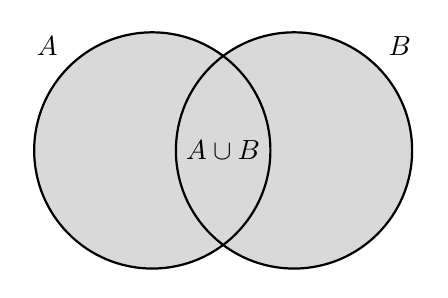
\begin{tikzpicture}[thick,
    set/.style = {circle,
        minimum size = 3cm,
        fill=black!15}]

% Set A
\node[set,label={135:$A$}] (A) at (0,0) {};

% Set B
\node[set,label={45:$B$}] (B) at (1.8,0) {};

% Intersection
\begin{scope}
    \clip (0,0) circle(1.5cm);
    \clip (1.8,0) circle(1.5cm);
    \fill[black!15](0,0) circle(1.5cm);
\end{scope}

% Circles outline
\draw (0,0) circle(1.5cm);
\draw (1.8,0) circle(1.5cm);

% Set intersection label
\node at (0.9,0) {$A\cup B$};

\end{tikzpicture}%
\hfill%
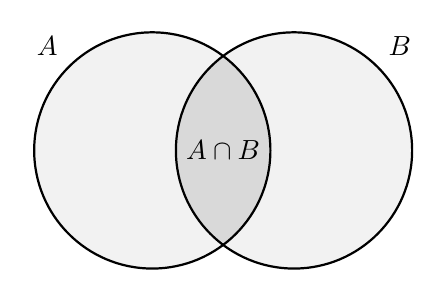
\begin{tikzpicture}[thick,
    set/.style = {circle,
        minimum size = 3cm,
        fill = black!5}]

% Set A
\node[set,label={135:$A$}] (A) at (0,0) {};

% Set B
\node[set,label={45:$B$}] (B) at (1.8,0) {};

% Intersection
\begin{scope}
    \clip (0,0) circle(1.5cm);
    \clip (1.8,0) circle(1.5cm);
    \fill[black!15](0,0) circle(1.5cm);
\end{scope}
% Circles outline
\draw (0,0) circle(1.5cm);
\draw (1.8,0) circle(1.5cm);

% Set intersection label
\node at (0.9,0) {$A\cap B$};

\end{tikzpicture}%
\hfill%
\vspace{2ex}

\hfill%
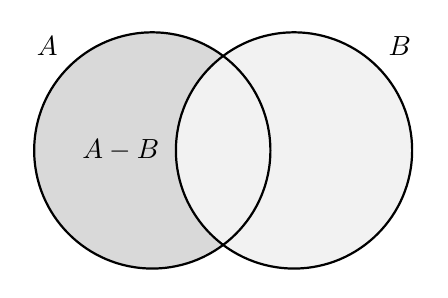
\begin{tikzpicture}[thick,
    set/.style = {circle,
        minimum size = 3cm}]

% Set A
\node[set,label={135:$A$},fill=black!15] (A) at (0,0) {};

% Set B
\node[set,label={45:$B$},fill=black!5] (B) at (1.8,0) {};

% Circles outline
\draw (0,0) circle(1.5cm);
\draw (1.8,0) circle(1.5cm);

% Set intersection label
\node at (-0.4,0) {$A - B$};

\end{tikzpicture}%
\hfill%
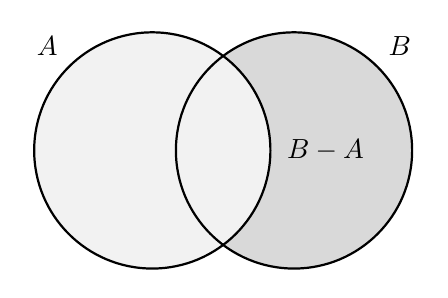
\begin{tikzpicture}[thick,
    set/.style = {circle,
        minimum size = 3cm}]

% Set B
\node[set,label={45:$B$},fill=black!15] (B) at (1.8,0) {};

% Set A
\node[set,label={135:$A$},fill=black!5] (A) at (0,0) {};

% Circles outline
\draw (0,0) circle(1.5cm);
\draw (1.8,0) circle(1.5cm);

% Set intersection label
\node at (2.2,0) {$B - A$};

\end{tikzpicture}%
\hfill%
\end{small}
\vspace{1ex}

The remaining operations are easier to exemplify using vectors with values representing a mundane example, grocery shopping, only later followed by more abstract examples.

\begin{knitrout}\footnotesize
\definecolor{shadecolor}{rgb}{0.969, 0.969, 0.969}\color{fgcolor}\begin{kframe}
\begin{alltt}
\hlstd{fruits} \hlkwb{<-} \hlkwd{c}\hlstd{(}\hlstr{"apple"}\hlstd{,} \hlstr{"pear"}\hlstd{,} \hlstr{"orange"}\hlstd{,} \hlstr{"lemon"}\hlstd{,} \hlstr{"tangerine"}\hlstd{)}
\hlstd{bakery} \hlkwb{<-} \hlkwd{c}\hlstd{(}\hlstr{"bread"}\hlstd{,} \hlstr{"buns"}\hlstd{,} \hlstr{"cake"}\hlstd{,} \hlstr{"cookies"}\hlstd{)}
\hlstd{dairy} \hlkwb{<-} \hlkwd{c}\hlstd{(}\hlstr{"milk"}\hlstd{,} \hlstr{"butter"}\hlstd{,} \hlstr{"cheese"}\hlstd{)}
\hlstd{shopping} \hlkwb{<-} \hlkwd{c}\hlstd{(}\hlstr{"bread"}\hlstd{,} \hlstr{"butter"}\hlstd{,} \hlstr{"apple"}\hlstd{,} \hlstr{"cheese"}\hlstd{,} \hlstr{"orange"}\hlstd{)}
\hlkwd{intersect}\hlstd{(fruits, shopping)}
\end{alltt}
\begin{verbatim}
## [1] "apple"  "orange"
\end{verbatim}
\begin{alltt}
\hlkwd{intersect}\hlstd{(bakery, shopping)}
\end{alltt}
\begin{verbatim}
## [1] "bread"
\end{verbatim}
\begin{alltt}
\hlkwd{intersect}\hlstd{(dairy, shopping)}
\end{alltt}
\begin{verbatim}
## [1] "butter" "cheese"
\end{verbatim}
\begin{alltt}
\hlstr{"lemon"} \hlopt \hlstd{dairy}
\end{alltt}
\begin{verbatim}
## [1] FALSE
\end{verbatim}
\begin{alltt}
\hlstr{"lemon"} \hlopt \hlstd{fruits}
\end{alltt}
\begin{verbatim}
## [1] TRUE
\end{verbatim}
\begin{alltt}
\hlstd{dairy} \hlopt \hlstd{shopping}
\end{alltt}
\begin{verbatim}
## [1] FALSE  TRUE  TRUE
\end{verbatim}
\begin{alltt}
\hlkwd{setdiff}\hlstd{(}\hlkwd{union}\hlstd{(bakery, dairy), shopping)}
\end{alltt}
\begin{verbatim}
## [1] "buns"    "cake"    "cookies" "milk"
\end{verbatim}
\end{kframe}
\end{knitrout}

\begin{warningbox}
  Sets describe membership as a binary property, thus when vectors are interpreted as sets, duplicate members are meaningless, although accepted as input and always simplified in the returned values.

\begin{knitrout}\footnotesize
\definecolor{shadecolor}{rgb}{0.969, 0.969, 0.969}\color{fgcolor}\begin{kframe}
\begin{alltt}
\hlkwd{setequal}\hlstd{(}\hlkwd{c}\hlstd{(}\hlstr{"a"}\hlstd{,} \hlstr{"a"}\hlstd{,} \hlstr{"b"}\hlstd{),} \hlkwd{c}\hlstd{(}\hlstr{"b"}\hlstd{,} \hlstr{"a"}\hlstd{,} \hlstr{"b"}\hlstd{))} \hlcom{# sets compared}
\end{alltt}
\begin{verbatim}
## [1] TRUE
\end{verbatim}
\begin{alltt}
\hlkwd{identical}\hlstd{(}\hlkwd{c}\hlstd{(}\hlstr{"a"}\hlstd{,} \hlstr{"a"}\hlstd{,} \hlstr{"b"}\hlstd{),} \hlkwd{c}\hlstd{(}\hlstr{"b"}\hlstd{,} \hlstr{"a"}\hlstd{,} \hlstr{"b"}\hlstd{))} \hlcom{# object compared}
\end{alltt}
\begin{verbatim}
## [1] FALSE
\end{verbatim}
\begin{alltt}
\hlkwd{union}\hlstd{(}\hlkwd{c}\hlstd{(}\hlstr{"a"}\hlstd{,} \hlstr{"a"}\hlstd{,} \hlstr{"b"}\hlstd{),} \hlkwd{c}\hlstd{(}\hlstr{"b"}\hlstd{,} \hlstr{"a"}\hlstd{,} \hlstr{"b"}\hlstd{))} \hlcom{# set operation}
\end{alltt}
\begin{verbatim}
## [1] "a" "b"
\end{verbatim}
\end{kframe}
\end{knitrout}
\end{warningbox}

We construct and save a character vector to use in the next examples.

\begin{knitrout}\footnotesize
\definecolor{shadecolor}{rgb}{0.969, 0.969, 0.969}\color{fgcolor}\begin{kframe}
\begin{alltt}
\hlstd{my.set} \hlkwb{<-} \hlkwd{c}\hlstd{(}\hlstr{"a"}\hlstd{,} \hlstr{"b"}\hlstd{,} \hlstr{"c"}\hlstd{,} \hlstr{"b"}\hlstd{)}
\end{alltt}
\end{kframe}
\end{knitrout}

To test if a given value belongs to a set, we use operator \Roperator{\%in\%} or its function equivalent \Rfunction{is.element()}. In the algebra of sets notation, this is written $a \in A$, where $A$ is a set and $a$ a member. The second statement shows that the \code{\%in\%} operator is vectorized on its left-hand-side (lhs) operand, returning a logical vector.

\begin{knitrout}\footnotesize
\definecolor{shadecolor}{rgb}{0.969, 0.969, 0.969}\color{fgcolor}\begin{kframe}
\begin{alltt}
\hlkwd{is.element}\hlstd{(}\hlstr{"a"}\hlstd{, my.set)}
\end{alltt}
\begin{verbatim}
## [1] TRUE
\end{verbatim}
\begin{alltt}
\hlstr{"a"} \hlopt \hlstd{my.set}
\end{alltt}
\begin{verbatim}
## [1] TRUE
\end{verbatim}
\begin{alltt}
\hlkwd{c}\hlstd{(}\hlstr{"a"}\hlstd{,} \hlstr{"a"}\hlstd{,} \hlstr{"z"}\hlstd{)} \hlopt \hlstd{my.set}
\end{alltt}
\begin{verbatim}
## [1]  TRUE  TRUE FALSE
\end{verbatim}
\end{kframe}
\end{knitrout}

\begin{explainbox}
Keep in mind that inclusion is an asymmetrical (not reflective) operation among sets. The rhs argument is interpreted as a set, while the lhs argument is interpreted as a vector of values to test for inclusion. In other words, any duplicate member in the lhs will be retained while the rhs is interpreted as a set of unique values. The returned logical vector has the same length as the lhs.
\begin{knitrout}\footnotesize
\definecolor{shadecolor}{rgb}{0.969, 0.969, 0.969}\color{fgcolor}\begin{kframe}
\begin{alltt}
\hlstd{my.set} \hlopt \hlstr{"a"}
\end{alltt}
\begin{verbatim}
## [1]  TRUE FALSE FALSE FALSE
\end{verbatim}
\end{kframe}
\end{knitrout}
\end{explainbox}

The negation of inclusion is $a \not\in A$, and coded in \Rlang by applying the negation operator \Roperator{!} to the result of the test done with \Roperator{\%in\%} or function \Rfunction{is.element()}.

\begin{knitrout}\footnotesize
\definecolor{shadecolor}{rgb}{0.969, 0.969, 0.969}\color{fgcolor}\begin{kframe}
\begin{alltt}
\hlopt{!}\hlkwd{is.element}\hlstd{(}\hlstr{"a"}\hlstd{, my.set)}
\end{alltt}
\begin{verbatim}
## [1] FALSE
\end{verbatim}
\begin{alltt}
\hlopt{!}\hlstr{"a"} \hlopt \hlstd{my.set}
\end{alltt}
\begin{verbatim}
## [1] FALSE
\end{verbatim}
\begin{alltt}
\hlopt{!}\hlkwd{c}\hlstd{(}\hlstr{"a"}\hlstd{,} \hlstr{"a"}\hlstd{,} \hlstr{"z"}\hlstd{)} \hlopt \hlstd{my.set}
\end{alltt}
\begin{verbatim}
## [1] FALSE FALSE  TRUE
\end{verbatim}
\end{kframe}
\end{knitrout}

Although inclusion is a set operation, it is also very useful for the simplification of \code{if () \ldots\ else} statements by replacing multiple tests for alternative constant values of the same \code{mode} chained by multiple \Roperator{|} operators. A useful property of \Roperator{\%in\%} and \Rfunction{is.element()} is that they never return \code{NA}.

\begin{playground}
Use operator \Roperator{\%in\%} to write more concisely the following comparisons. Hint: see section \ref{sec:calc:boolean} on page \pageref{sec:calc:boolean} for the difference between \code{|} and \code{||} operators.

\begin{knitrout}\footnotesize
\definecolor{shadecolor}{rgb}{0.969, 0.969, 0.969}\color{fgcolor}\begin{kframe}
\begin{alltt}
\hlstd{x} \hlkwb{<-} \hlkwd{c}\hlstd{(}\hlstr{"a"}\hlstd{,} \hlstr{"a"}\hlstd{,} \hlstr{"z"}\hlstd{)}
\hlstd{x} \hlopt{==} \hlstr{"a"} \hlopt{|} \hlstd{x} \hlopt{==} \hlstr{"b"} \hlopt{|} \hlstd{x} \hlopt{==} \hlstr{"c"} \hlopt{|} \hlstd{x} \hlopt{==} \hlstr{"d"}
\end{alltt}
\end{kframe}
\end{knitrout}

Convert the \code{logical} vectors of length 3 into a vector of length one. Hint: see help for functions \code{all()} and \code{any()}.
\end{playground}

With \Rfunction{unique()} we convert a vector of possibly repeated values into a set of unique values. In the algebra of sets, a certain object belongs or not to a set. Consequently, in a set, multiple copies of the same object or value are meaningless.

\begin{knitrout}\footnotesize
\definecolor{shadecolor}{rgb}{0.969, 0.969, 0.969}\color{fgcolor}\begin{kframe}
\begin{alltt}
\hlkwd{unique}\hlstd{(my.set)}
\end{alltt}
\begin{verbatim}
## [1] "a" "b" "c"
\end{verbatim}
\begin{alltt}
\hlkwd{c}\hlstd{(}\hlstr{"a"}\hlstd{,} \hlstr{"a"}\hlstd{,} \hlstr{"z"}\hlstd{)} \hlopt \hlkwd{unique}\hlstd{(my.set)}
\end{alltt}
\begin{verbatim}
## [1]  TRUE  TRUE FALSE
\end{verbatim}
\end{kframe}
\end{knitrout}

In the notation used in algebra of sets, the set union operator is $\cup$ while the intersection operator is $\cap$. If we have sets $A$ and $B$, their union is given by $A \cup B$---in the next three examples, \code{c("a", "a", "z")} is a constant, while \code{my.set} is a variable.

\begin{knitrout}\footnotesize
\definecolor{shadecolor}{rgb}{0.969, 0.969, 0.969}\color{fgcolor}\begin{kframe}
\begin{alltt}
\hlkwd{union}\hlstd{(}\hlkwd{c}\hlstd{(}\hlstr{"a"}\hlstd{,} \hlstr{"a"}\hlstd{,} \hlstr{"z"}\hlstd{), my.set)}
\end{alltt}
\begin{verbatim}
## [1] "a" "z" "b" "c"
\end{verbatim}
\end{kframe}
\end{knitrout}

If we have sets $A$ and $B$, their intersection is given by $A \cap B$.

\begin{knitrout}\footnotesize
\definecolor{shadecolor}{rgb}{0.969, 0.969, 0.969}\color{fgcolor}\begin{kframe}
\begin{alltt}
\hlkwd{intersect}\hlstd{(}\hlkwd{c}\hlstd{(}\hlstr{"a"}\hlstd{,} \hlstr{"a"}\hlstd{,} \hlstr{"z"}\hlstd{), my.set)}
\end{alltt}
\begin{verbatim}
## [1] "a"
\end{verbatim}
\end{kframe}
\end{knitrout}

\begin{playground}
What do you expect to be the difference between the values returned by the three statements in the code chunk below? Before running them, write down your expectations about the value each one will return. Only then run the code. Independently of whether your predictions were correct or not, write down an explanation of what each statement's operation is.

\begin{knitrout}\footnotesize
\definecolor{shadecolor}{rgb}{0.969, 0.969, 0.969}\color{fgcolor}\begin{kframe}
\begin{alltt}
\hlkwd{union}\hlstd{(}\hlkwd{c}\hlstd{(}\hlstr{"a"}\hlstd{,} \hlstr{"a"}\hlstd{,} \hlstr{"z"}\hlstd{), my.set)}
\hlkwd{c}\hlstd{(}\hlkwd{c}\hlstd{(}\hlstr{"a"}\hlstd{,} \hlstr{"a"}\hlstd{,} \hlstr{"z"}\hlstd{), my.set)}
\hlkwd{c}\hlstd{(}\hlstr{"a"}\hlstd{,} \hlstr{"a"}\hlstd{,} \hlstr{"z"}\hlstd{, my.set)}
\end{alltt}
\end{kframe}
\end{knitrout}

In the algebra of sets notation $A \subseteq B$, where $A$ and $B$ are sets, indicates that $A$ is a subset or equal to $B$. For a true subset, the notation is $A \subset B$. The operators with the reverse direction are $\supseteq$ and $\supset$. Implement these four operations in four \Rlang statements, and test them on sets (represented by \Rlang vectors) with different ``overlap'' among set members.

\end{playground}

\begin{explainbox}
All set algebra examples above use character vectors and character constants. This is just the most frequent use case. Sets operations are valid on vectors of any atomic class, including \code{integer}, and computed values can be part of statements. In the second and third statements in the next chunk, we need to use additional parentheses to alter the default order of precedence between arithmetic and set operators.

\begin{knitrout}\footnotesize
\definecolor{shadecolor}{rgb}{0.969, 0.969, 0.969}\color{fgcolor}\begin{kframe}
\begin{alltt}
\hlnum{9L} \hlopt \hlnum{2L}\hlopt{:}\hlnum{4L}
\end{alltt}
\begin{verbatim}
## [1] FALSE
\end{verbatim}
\begin{alltt}
\hlnum{9L} \hlopt \hlstd{((}\hlnum{2L}\hlopt{:}\hlnum{4L}\hlstd{)} \hlopt{*} \hlstd{(}\hlnum{2L}\hlopt{:}\hlnum{4L}\hlstd{))}
\end{alltt}
\begin{verbatim}
## [1] TRUE
\end{verbatim}
\begin{alltt}
\hlkwd{c}\hlstd{(}\hlnum{1L}\hlstd{,} \hlnum{16L}\hlstd{)} \hlopt \hlstd{((}\hlnum{2L}\hlopt{:}\hlnum{4L}\hlstd{)} \hlopt{*} \hlstd{(}\hlnum{2L}\hlopt{:}\hlnum{4L}\hlstd{))}
\end{alltt}
\begin{verbatim}
## [1] FALSE  TRUE
\end{verbatim}
\end{kframe}
\end{knitrout}

\emph{Empty sets} are an important component of the algebra of sets, in \Rlang they are represented as vectors of zero length. Vectors and lists of zero length, which the \Rlang language fully supports, can be used to ``encode'' emptiness also in other contexts. These vectors do belong to a class such as \Rclass{numeric} or \Rclass{character} and must be compatible with other operands in an expression. By default, constructors for vectors, construct empty vectors.

\begin{knitrout}\footnotesize
\definecolor{shadecolor}{rgb}{0.969, 0.969, 0.969}\color{fgcolor}\begin{kframe}
\begin{alltt}
\hlkwd{length}\hlstd{(}\hlkwd{integer}\hlstd{())}
\end{alltt}
\begin{verbatim}
## [1] 0
\end{verbatim}
\end{kframe}
\end{knitrout}

\begin{knitrout}\footnotesize
\definecolor{shadecolor}{rgb}{0.969, 0.969, 0.969}\color{fgcolor}\begin{kframe}
\begin{alltt}
\hlnum{1L} \hlopt \hlkwd{integer}\hlstd{()}
\end{alltt}
\begin{verbatim}
## [1] FALSE
\end{verbatim}
\begin{alltt}
\hlkwd{setdiff}\hlstd{(}\hlnum{1L}\hlopt{:}\hlnum{4L}\hlstd{,} \hlkwd{union}\hlstd{(}\hlnum{1L}\hlopt{:}\hlnum{4L}\hlstd{,} \hlkwd{integer}\hlstd{()))}
\end{alltt}
\begin{verbatim}
## integer(0)
\end{verbatim}
\end{kframe}
\end{knitrout}

Although set operators are defined for \Rclass{numeric} vectors, rounding errors in `floats' can result in unexpected results (see section \ref{box:floats} on page \pageref{box:floats}). The next two examples do, however, return the correct answers.\qRoperator{\%in\%}

\begin{knitrout}\footnotesize
\definecolor{shadecolor}{rgb}{0.969, 0.969, 0.969}\color{fgcolor}\begin{kframe}
\begin{alltt}
\hlnum{9} \hlopt \hlstd{(}\hlnum{2}\hlopt{:}\hlnum{4}\hlstd{)}\hlopt{^}\hlnum{2}
\end{alltt}
\begin{verbatim}
## [1] TRUE
\end{verbatim}
\begin{alltt}
\hlkwd{c}\hlstd{(}\hlnum{1}\hlstd{,} \hlnum{5}\hlstd{)} \hlopt \hlstd{(}\hlnum{1}\hlopt{:}\hlnum{10}\hlstd{)}\hlopt{^}\hlnum{2}
\end{alltt}
\begin{verbatim}
## [1]  TRUE FALSE
\end{verbatim}
\end{kframe}
\end{knitrout}

\end{explainbox}
\index{operators!set|)}
\index{sets|)}

\section{Character values}\label{sec:calc:character}
\index{character strings}\index{classes and modes!character|(}\qRclass{character}
Character variables can be used to store any character. Character constants are written by enclosing characters in quotes. There are three types of quotes in the ASCII character set, double quotes \code{"}, single quotes \code{'}, and back ticks \code{`}. The first two types of quotes can be used as delimiters of \code{character} constants.

\begin{knitrout}\footnotesize
\definecolor{shadecolor}{rgb}{0.969, 0.969, 0.969}\color{fgcolor}\begin{kframe}
\begin{alltt}
\hlstd{a} \hlkwb{<-} \hlstr{"A"}
\hlstd{a}
\end{alltt}
\begin{verbatim}
## [1] "A"
\end{verbatim}
\begin{alltt}
\hlstd{b} \hlkwb{<-} \hlstr{'A'}
\hlstd{b}
\end{alltt}
\begin{verbatim}
## [1] "A"
\end{verbatim}
\begin{alltt}
\hlstd{a} \hlopt{==} \hlstd{b}
\end{alltt}
\begin{verbatim}
## [1] TRUE
\end{verbatim}
\end{kframe}
\end{knitrout}

\begin{explainbox}
In many computer languages, vectors of characters are distinct from vectors of character strings. In these languages, character vectors store at each index position a single character, while vectors of character strings store at each index position strings of characters of various lengths, such as words or sentences. If you are familiar with \Clang or \Cpplang, you need to keep in mind that \Clang's \code{char} and \Rlang's \code{character} are not equivalent and that in \Rlang, \code{character} vectors are vectors of character strings. In contrast to these other languages, in \Rlang there is no predefined class for vectors of individual characters and character constants enclosed in double or single quotes are not different.
\end{explainbox}

Concatenating character vectors of length one does not yield a longer character string, it yields instead a longer vector.
\begin{knitrout}\footnotesize
\definecolor{shadecolor}{rgb}{0.969, 0.969, 0.969}\color{fgcolor}\begin{kframe}
\begin{alltt}
\hlstd{a} \hlkwb{<-} \hlstr{'A'}
\hlstd{b} \hlkwb{<-} \hlstr{"bcdefg"}
\hlstd{c} \hlkwb{<-} \hlstr{"123"}
\hlstd{d} \hlkwb{<-} \hlkwd{c}\hlstd{(a, b, c)}
\hlstd{d}
\end{alltt}
\begin{verbatim}
## [1] "A"      "bcdefg" "123"
\end{verbatim}
\end{kframe}
\end{knitrout}

Having two different delimiters available makes it possible to choose the type of quotes used as delimiters so that other quotes can be included in a string.

\begin{knitrout}\footnotesize
\definecolor{shadecolor}{rgb}{0.969, 0.969, 0.969}\color{fgcolor}\begin{kframe}
\begin{alltt}
\hlstd{a} \hlkwb{<-} \hlstr{"He said 'hello' when he came in"}
\hlstd{a}
\end{alltt}
\begin{verbatim}
## [1] "He said 'hello' when he came in"
\end{verbatim}
\begin{alltt}
\hlstd{b} \hlkwb{<-} \hlstr{'He said "hello" when he came in'}
\hlstd{b}
\end{alltt}
\begin{verbatim}
## [1] "He said \"hello\" when he came in"
\end{verbatim}
\end{kframe}
\end{knitrout}

The\index{character string delimiters} outer quotes are not part of the string, they are ``delimiters'' used to mark the boundaries. As you can see when \code{b} is printed special characters can be represented using ``escape sequences''. There are several of them, and here we will show just four, new line (\verb|\n|) and tab (\verb|\t|), \verb|\"| the escape code for a quotation mark within a string and \verb|\\| the escape code for a single backslash \verb|\|. We also show here the different behavior of \Rfunction{print()} and \Rfunction{cat()}, with \Rfunction{cat()} \emph{interpreting} the escape sequences and \Rfunction{print()} displaying them as entered.

\begin{knitrout}\footnotesize
\definecolor{shadecolor}{rgb}{0.969, 0.969, 0.969}\color{fgcolor}\begin{kframe}
\begin{alltt}
\hlstd{c} \hlkwb{<-} \hlstr{"abc\textbackslash{}ndef\textbackslash{}tx\textbackslash{}"yz\textbackslash{}"\textbackslash{}\textbackslash{}\textbackslash{}tm"}
\hlkwd{print}\hlstd{(c)}
\end{alltt}
\begin{verbatim}
## [1] "abc\ndef\tx\"yz\"\\\tm"
\end{verbatim}
\begin{alltt}
\hlkwd{cat}\hlstd{(c)}
\end{alltt}
\begin{verbatim}
## abc
## def	x"yz"\	m
\end{verbatim}
\end{kframe}
\end{knitrout}

The \textit{escape codes}\index{character escape codes} work only in some contexts, as when using \Rfunction{cat()} to generate the output. For example, the new-line escape (\verb|\n|) can be embedded in strings used for axis-label, title or label in a plot to split them over two or more lines.
\index{classes and modes!character|)}

\section{The `mode' and `class' of objects}\label{sec:rlang:mode}
\index{objects!mode}
Variables have a \emph{mode} that depends on what is stored in them. But different from other languages, assignment to a variable of a different mode is allowed and in most cases its mode changes together with its contents. However, there is a restriction that all elements in a vector, array or matrix, must be of the same mode. While this is not required for lists, which can be heterogenous. In practice this means that we can assign an object, such as a vector, with a different \code{mode} to a name already in use, but we cannot use indexing to assign an object of a different mode to individual members of a vector, matrix or array. Functions with names starting with \code{is.} are tests returning a logical value, \code{TRUE}, \code{FALSE} or \code{NA}. Function \Rfunction{mode()} returns the mode of an object, as a character string and \Rfunction{typeof()} returns R's internal type or storage mode.\qRfunction{is.character()}\qRfunction{is.numeric()}\qRfunction{is.logical()}

\begin{knitrout}\footnotesize
\definecolor{shadecolor}{rgb}{0.969, 0.969, 0.969}\color{fgcolor}\begin{kframe}
\begin{alltt}
\hlstd{my_var} \hlkwb{<-} \hlnum{1}\hlopt{:}\hlnum{5}
\hlkwd{mode}\hlstd{(my_var)} \hlcom{# no distinction of integer or double}
\end{alltt}
\begin{verbatim}
## [1] "numeric"
\end{verbatim}
\begin{alltt}
\hlkwd{typeof}\hlstd{(my_var)}
\end{alltt}
\begin{verbatim}
## [1] "integer"
\end{verbatim}
\begin{alltt}
\hlkwd{is.numeric}\hlstd{(my_var)} \hlcom{# no distinction of integer or double}
\end{alltt}
\begin{verbatim}
## [1] TRUE
\end{verbatim}
\begin{alltt}
\hlkwd{is.double}\hlstd{(my_var)}
\end{alltt}
\begin{verbatim}
## [1] FALSE
\end{verbatim}
\begin{alltt}
\hlkwd{is.integer}\hlstd{(my_var)}
\end{alltt}
\begin{verbatim}
## [1] TRUE
\end{verbatim}
\begin{alltt}
\hlkwd{is.logical}\hlstd{(my_var)}
\end{alltt}
\begin{verbatim}
## [1] FALSE
\end{verbatim}
\begin{alltt}
\hlkwd{is.character}\hlstd{(my_var)}
\end{alltt}
\begin{verbatim}
## [1] FALSE
\end{verbatim}
\begin{alltt}
\hlstd{my_var} \hlkwb{<-} \hlstr{"abc"}
\hlkwd{mode}\hlstd{(my_var)}
\end{alltt}
\begin{verbatim}
## [1] "character"
\end{verbatim}
\end{kframe}
\end{knitrout}

While \emph{mode} is a fundamental property, and limited to those modes defined as part of the \Rlang language, the concept of \emph{class}, is different in that new classes can be defined in user code. In particular, different \Rlang objects of a given mode, such as \code{numeric}, can belong to different \code{class}es. The use of classes for dispatching functions is discussed in section \ref{sec:script:objects:classes:methods} on page \pageref{sec:script:objects:classes:methods}, in relation to object-oriented programming in \Rlang. Method \Rfunction{class()} is used to query the class of an object, and method \Rfunction{inherits()} is used to test if an object belongs to a specific class or not (including ``parent'' classes, to be later described).

\begin{knitrout}\footnotesize
\definecolor{shadecolor}{rgb}{0.969, 0.969, 0.969}\color{fgcolor}\begin{kframe}
\begin{alltt}
\hlkwd{class}\hlstd{(my_var)}
\end{alltt}
\begin{verbatim}
## [1] "character"
\end{verbatim}
\begin{alltt}
\hlkwd{inherits}\hlstd{(my_var,} \hlstr{"character"}\hlstd{)}
\end{alltt}
\begin{verbatim}
## [1] TRUE
\end{verbatim}
\begin{alltt}
\hlkwd{inherits}\hlstd{(my_var,} \hlstr{"numeric"}\hlstd{)}
\end{alltt}
\begin{verbatim}
## [1] FALSE
\end{verbatim}
\end{kframe}
\end{knitrout}

\section{`Type' conversions}\label{sec:calc:type:conversion}
\index{type conversion|(}
The least-intuitive type conversions are those related to logical values. All others are as one would expect. By convention, functions used to convert objects from one mode to a different one have names starting with \code{as.}\footnote{Except for some packages in the \pkgnameNI{tidyverse} that use names starting with \code{as\_} instead of \code{as.}.}.\qRfunction{as.character()}\qRfunction{as.numeric()}\qRfunction{as.logical()}

\begin{knitrout}\footnotesize
\definecolor{shadecolor}{rgb}{0.969, 0.969, 0.969}\color{fgcolor}\begin{kframe}
\begin{alltt}
\hlkwd{as.character}\hlstd{(}\hlnum{1}\hlstd{)}
\end{alltt}
\begin{verbatim}
## [1] "1"
\end{verbatim}
\begin{alltt}
\hlkwd{as.numeric}\hlstd{(}\hlstr{"1"}\hlstd{)}
\end{alltt}
\begin{verbatim}
## [1] 1
\end{verbatim}
\begin{alltt}
\hlkwd{as.logical}\hlstd{(}\hlstr{"TRUE"}\hlstd{)}
\end{alltt}
\begin{verbatim}
## [1] TRUE
\end{verbatim}
\begin{alltt}
\hlkwd{as.logical}\hlstd{(}\hlstr{"NA"}\hlstd{)}
\end{alltt}
\begin{verbatim}
## [1] NA
\end{verbatim}
\end{kframe}
\end{knitrout}

Conversion takes place automatically in arithmetic and logical expressions.

\begin{knitrout}\footnotesize
\definecolor{shadecolor}{rgb}{0.969, 0.969, 0.969}\color{fgcolor}\begin{kframe}
\begin{alltt}
\hlnum{TRUE} \hlopt{+} \hlnum{10}
\end{alltt}
\begin{verbatim}
## [1] 11
\end{verbatim}
\begin{alltt}
\hlnum{1} \hlopt{||} \hlnum{0}
\end{alltt}
\begin{verbatim}
## [1] TRUE
\end{verbatim}
\begin{alltt}
\hlnum{FALSE} \hlopt{| -}\hlnum{2}\hlopt{:}\hlnum{2}
\end{alltt}
\begin{verbatim}
## [1]  TRUE  TRUE FALSE  TRUE  TRUE
\end{verbatim}
\end{kframe}
\end{knitrout}

\begin{playground}
There is some flexibility in the conversion from character strings into \code{numeric} and \code{logical} values. Use the examples below plus your own variations to get an idea of what strings are acceptable and correctly converted and which are not. Do also pay attention at the conversion between \code{numeric} and \code{logical} values.\qRfunction{as.character()}\qRfunction{as.numeric()}\qRfunction{as.logical()}

\begin{knitrout}\footnotesize
\definecolor{shadecolor}{rgb}{0.969, 0.969, 0.969}\color{fgcolor}\begin{kframe}
\begin{alltt}
\hlkwd{as.character}\hlstd{(}\hlnum{3.0e10}\hlstd{)}
\hlkwd{as.numeric}\hlstd{(}\hlstr{"5E+5"}\hlstd{)}
\hlkwd{as.numeric}\hlstd{(}\hlstr{"A"}\hlstd{)}
\hlkwd{as.numeric}\hlstd{(}\hlnum{TRUE}\hlstd{)}
\hlkwd{as.numeric}\hlstd{(}\hlnum{FALSE}\hlstd{)}
\hlkwd{as.logical}\hlstd{(}\hlstr{"T"}\hlstd{)}
\hlkwd{as.logical}\hlstd{(}\hlstr{"t"}\hlstd{)}
\hlkwd{as.logical}\hlstd{(}\hlstr{"true"}\hlstd{)}
\hlkwd{as.logical}\hlstd{(}\hlnum{100}\hlstd{)}
\hlkwd{as.logical}\hlstd{(}\hlnum{0}\hlstd{)}
\hlkwd{as.logical}\hlstd{(}\hlopt{-}\hlnum{1}\hlstd{)}
\end{alltt}
\end{kframe}
\end{knitrout}

\end{playground}

\begin{playground}
Compare the values returned by \Rfunction{trunc()} and \Rfunction{as.integer()} when applied to a floating point number, such as \code{12.34}. Check for the equality of values, and for the \emph{class} of the returned objects.
\end{playground}

\begin{explainbox}
Using conversions, the difference between the length of a \code{character} vector and the number of characters composing each member ``string'' within a vector is obvious.\qRfunction{length()}\qRfunction{as.numeric()}

\begin{knitrout}\footnotesize
\definecolor{shadecolor}{rgb}{0.969, 0.969, 0.969}\color{fgcolor}\begin{kframe}
\begin{alltt}
\hlstd{f} \hlkwb{<-} \hlkwd{c}\hlstd{(}\hlstr{"1"}\hlstd{,} \hlstr{"2"}\hlstd{,} \hlstr{"3"}\hlstd{)}
\hlkwd{length}\hlstd{(f)}
\end{alltt}
\begin{verbatim}
## [1] 3
\end{verbatim}
\begin{alltt}
\hlstd{g} \hlkwb{<-} \hlstr{"123"}
\hlkwd{length}\hlstd{(g)}
\end{alltt}
\begin{verbatim}
## [1] 1
\end{verbatim}
\begin{alltt}
\hlkwd{as.numeric}\hlstd{(f)}
\end{alltt}
\begin{verbatim}
## [1] 1 2 3
\end{verbatim}
\begin{alltt}
\hlkwd{as.numeric}\hlstd{(g)}
\end{alltt}
\begin{verbatim}
## [1] 123
\end{verbatim}
\end{kframe}
\end{knitrout}
\end{explainbox}

\sloppy
Other\index{formatted character strings from numbers} functions relevant to the ``conversion'' of numbers and other values are \Rfunction{format()}, and \Rfunction{sprintf()}. These two functions return \Rclass{character} strings, instead of \code{numeric} or other values, and are useful for printing output. One could think of these functions as advanced conversion functions returning formatted, and possibly combined and annotated, character strings. However, they are usually not considered normal conversion functions, as they are very rarely used in a way that preserves the original precision of the input values. We show here the use of \Rfunction{format()} and \Rfunction{sprintf()} with \code{numeric} values, but they can also be used with values of other modes.

When using \Rfunction{format()}, the format used to display numbers is set by passing arguments to several different parameters. As \Rfunction{print()} calls \Rfunction{format()} to make numbers \emph{pretty} it accepts the same options.

\begin{knitrout}\footnotesize
\definecolor{shadecolor}{rgb}{0.969, 0.969, 0.969}\color{fgcolor}\begin{kframe}
\begin{alltt}
\hlstd{x} \hlkwb{=} \hlkwd{c}\hlstd{(}\hlnum{123.4567890}\hlstd{,} \hlnum{1.0}\hlstd{)}
\hlkwd{format}\hlstd{(x)} \hlcom{# using defaults}
\end{alltt}
\begin{verbatim}
## [1] "123.4568" "  1.0000"
\end{verbatim}
\begin{alltt}
\hlkwd{format}\hlstd{(x[}\hlnum{1}\hlstd{])} \hlcom{# using defaults}
\end{alltt}
\begin{verbatim}
## [1] "123.4568"
\end{verbatim}
\begin{alltt}
\hlkwd{format}\hlstd{(x[}\hlnum{2}\hlstd{])} \hlcom{# using defaults}
\end{alltt}
\begin{verbatim}
## [1] "1"
\end{verbatim}
\begin{alltt}
\hlkwd{format}\hlstd{(x,} \hlkwc{digits} \hlstd{=} \hlnum{3}\hlstd{,} \hlkwc{nsmall} \hlstd{=} \hlnum{1}\hlstd{)}
\end{alltt}
\begin{verbatim}
## [1] "123.5" "  1.0"
\end{verbatim}
\begin{alltt}
\hlkwd{format}\hlstd{(x[}\hlnum{1}\hlstd{],} \hlkwc{digits} \hlstd{=} \hlnum{3}\hlstd{,} \hlkwc{nsmall} \hlstd{=} \hlnum{1}\hlstd{)}
\end{alltt}
\begin{verbatim}
## [1] "123.5"
\end{verbatim}
\begin{alltt}
\hlkwd{format}\hlstd{(x[}\hlnum{2}\hlstd{],} \hlkwc{digits} \hlstd{=} \hlnum{3}\hlstd{,} \hlkwc{nsmall} \hlstd{=} \hlnum{1}\hlstd{)}
\end{alltt}
\begin{verbatim}
## [1] "1.0"
\end{verbatim}
\begin{alltt}
\hlkwd{format}\hlstd{(x,} \hlkwc{digits} \hlstd{=} \hlnum{3}\hlstd{,} \hlkwc{scientific} \hlstd{=} \hlnum{TRUE}\hlstd{)}
\end{alltt}
\begin{verbatim}
## [1] "1.23e+02" "1.00e+00"
\end{verbatim}
\end{kframe}
\end{knitrout}

Function \Rfunction{sprintf()} is similar to \Clang's function of the same name. The user interface is rather unusual, but very powerful, once one learns the syntax. All the formatting is specified using a \code{character} string as template. In this template, placeholders for data and the formatting instructions are embedded using special codes. These codes start with a percent character. We show in the example below the use of some of these: \code{f} is used for \code{numeric} values to be formatted according to a ``fixed point,'' while \code{g} is used when we set the number of significant digits and \code{e} for exponential or \emph{scientific} notation.

\begin{knitrout}\footnotesize
\definecolor{shadecolor}{rgb}{0.969, 0.969, 0.969}\color{fgcolor}\begin{kframe}
\begin{alltt}
\hlstd{x} \hlkwb{=} \hlkwd{c}\hlstd{(}\hlnum{123.4567890}\hlstd{,} \hlnum{1.0}\hlstd{)}
\hlkwd{sprintf}\hlstd{(}\hlstr{"The numbers are: %4.2f and %.0f"}\hlstd{, x[}\hlnum{1}\hlstd{], x[}\hlnum{2}\hlstd{])}
\end{alltt}
\begin{verbatim}
## [1] "The numbers are: 123.46 and 1"
\end{verbatim}
\begin{alltt}
\hlkwd{sprintf}\hlstd{(}\hlstr{"The numbers are: %.4g and %.2g"}\hlstd{, x[}\hlnum{1}\hlstd{], x[}\hlnum{2}\hlstd{])}
\end{alltt}
\begin{verbatim}
## [1] "The numbers are: 123.5 and 1"
\end{verbatim}
\begin{alltt}
\hlkwd{sprintf}\hlstd{(}\hlstr{"The numbers are: %4.2e and %.0e"}\hlstd{, x[}\hlnum{1}\hlstd{], x[}\hlnum{2}\hlstd{])}
\end{alltt}
\begin{verbatim}
## [1] "The numbers are: 1.23e+02 and 1e+00"
\end{verbatim}
\end{kframe}
\end{knitrout}

In the template \code{"The numbers are: \%4.2f and \%.0f"}, there are two placeholders for \code{numeric} values, \code{\%4.2f} and \code{\%.0f}, so in addition to the template, we pass two values extracted from the first two positions of vector \code{x}. These could have been two different vectors of length one, or even numeric constants. The template itself does not need to be a \code{character} constant as in these examples, as a variable can be also passed as argument.

\begin{playground}
Function \Rfunction{format()} may be easier to use, in some cases, but \Rfunction{sprintf()} is more flexible and powerful. Those with experience in the use of the \Clang language will already know about \Rfunction{sprintf()} and its use of templates for formatting output. Even if you are familiar with  \Clang, look up the help pages for both functions, and practice, by trying to create the same formatted output by means of the two functions. Do also play with these functions with other types of data like \code{integer} and \code{character}.
\end{playground}

\begin{explainbox}
We have above described \Rconst{NA} as a single value ignoring modes, but in reality \Rconst{NA}s come in various flavors. \Rconst{NA\_real\_}, \Rconst{NA\_character\_}, etc. and \Rconst{NA} defaults to an \Rconst{NA} of class \Rclass{logical}. \Rconst{NA} is normally converted on the fly to other modes when needed, so in general \Rconst{NA} is all we need to use.

\begin{knitrout}\footnotesize
\definecolor{shadecolor}{rgb}{0.969, 0.969, 0.969}\color{fgcolor}\begin{kframe}
\begin{alltt}
\hlstd{a} \hlkwb{<-} \hlkwd{c}\hlstd{(}\hlnum{1}\hlstd{,} \hlnum{NA}\hlstd{)}
\hlkwd{is.numeric}\hlstd{(a[}\hlnum{2}\hlstd{])}
\end{alltt}
\begin{verbatim}
## [1] TRUE
\end{verbatim}
\begin{alltt}
\hlkwd{is.numeric}\hlstd{(}\hlnum{NA}\hlstd{)}
\end{alltt}
\begin{verbatim}
## [1] FALSE
\end{verbatim}
\end{kframe}
\end{knitrout}

\begin{knitrout}\footnotesize
\definecolor{shadecolor}{rgb}{0.969, 0.969, 0.969}\color{fgcolor}\begin{kframe}
\begin{alltt}
\hlstd{b} \hlkwb{<-} \hlkwd{c}\hlstd{(}\hlstr{"abc"}\hlstd{,} \hlnum{NA}\hlstd{)}
\hlkwd{is.character}\hlstd{(b[}\hlnum{2}\hlstd{])}
\end{alltt}
\begin{verbatim}
## [1] TRUE
\end{verbatim}
\end{kframe}
\end{knitrout}

\begin{knitrout}\footnotesize
\definecolor{shadecolor}{rgb}{0.969, 0.969, 0.969}\color{fgcolor}\begin{kframe}
\begin{alltt}
\hlkwd{is.character}\hlstd{(}\hlnum{NA}\hlstd{)}
\end{alltt}
\begin{verbatim}
## [1] FALSE
\end{verbatim}
\begin{alltt}
\hlkwd{class}\hlstd{(}\hlnum{NA}\hlstd{)}
\end{alltt}
\begin{verbatim}
## [1] "logical"
\end{verbatim}
\begin{alltt}
\hlkwd{class}\hlstd{(}\hlnum{NA_character_}\hlstd{)}
\end{alltt}
\begin{verbatim}
## [1] "character"
\end{verbatim}
\end{kframe}
\end{knitrout}

\begin{knitrout}\footnotesize
\definecolor{shadecolor}{rgb}{0.969, 0.969, 0.969}\color{fgcolor}\begin{kframe}
\begin{alltt}
\hlstd{c} \hlkwb{<-} \hlnum{NA}
\hlkwd{c}\hlstd{(c,} \hlnum{2}\hlopt{:}\hlnum{3}\hlstd{)}
\end{alltt}
\begin{verbatim}
## [1] NA  2  3
\end{verbatim}
\end{kframe}
\end{knitrout}

However, even the statement below works transparently.

\begin{knitrout}\footnotesize
\definecolor{shadecolor}{rgb}{0.969, 0.969, 0.969}\color{fgcolor}\begin{kframe}
\begin{alltt}
\hlstd{a[}\hlnum{3}\hlstd{]} \hlkwb{<-} \hlstd{b[}\hlnum{2}\hlstd{]}
\end{alltt}
\end{kframe}
\end{knitrout}
\end{explainbox}

\index{type conversion|)}

\section{Vector manipulation}\label{sec:vectors}\label{sec:calc:indexing}
\index{vectors!indexing|(}\index{vectors!member extraction}
If you have read earlier sections of this chapter, you already know how to create a vector. If not, see pages \pageref{par:numeric:vectors:start}--\pageref{par:numeric:vectors:end} before continuing.

In this section we are going to see how to extract or retrieve, replace, and move elements such as $a_2$ from a vector $a_{1 = 1\ldots n}$. Elements are extracted using an index enclosed in single square brackets. The index indicates the position in the vector, starting from one, following the usual mathematical tradition. What in maths notation would be $a_i$, in \Rpgrm is represented as \code{a[i]} and the whole vector, by excluding the brackets and indexing vector, as \code{a}.

We extract the first 10 elements of the vector \code{letters}.

\begin{knitrout}\footnotesize
\definecolor{shadecolor}{rgb}{0.969, 0.969, 0.969}\color{fgcolor}\begin{kframe}
\begin{alltt}
\hlstd{a} \hlkwb{<-} \hlstd{letters[}\hlnum{1}\hlopt{:}\hlnum{10}\hlstd{]}
\hlstd{a}
\end{alltt}
\begin{verbatim}
##  [1] "a" "b" "c" "d" "e" "f" "g" "h" "i" "j"
\end{verbatim}
\end{kframe}
\end{knitrout}

\begin{center}
\begin{small}
\begin{tikzpicture}[font=\sffamily,
array/.style={matrix of nodes,nodes={draw, minimum size=7mm, fill=red!20},column sep=-\pgflinewidth, row sep=0.5mm, nodes in empty cells,
row 1/.style={nodes={draw=none, fill=none, minimum size=5mm}},
row 1 column 2/.style={nodes={draw}}}]

\matrix[array] (array) {
1 & 2 & 3 & 4 & 5 & 6 & 7 & 8 & 9 & 10\\
``a''\strut & ``b''\strut & ``c''\strut & ``d''\strut & ``e''\strut & ``f''\strut & ``g''"\strut &``h''\strut & ``i''\strut & ``j''\strut \\};
\node[draw, minimum size=4mm] at (array-2-2) (box) {};

\begin{scope}[on background layer]
\fill[blue!10] (array-1-1.north west) rectangle (array-1-10.south east);
\end{scope}

\draw (array-2-1.west) node [signal, draw, fill=codeshadecolor, minimum size=6mm, line width=1.5pt, left] (first) {\code{\strut\ a\phantom{mmmm}}};
%\draw (array-1-2.north)--++(90:3mm) node [above] (first) {Index};
\draw (array-1-10.east)--++(0:3mm) node [right]{\code{integer} positional indices};
\draw (array-2-10.east)--++(0:3mm) node [right]{\code{character} values};
\node [align=center, anchor=south] at (array-2-2.south west|-first.south) (1) [below, yshift=-5mm]{\code{a[2]}};
\draw (1)--(box);
%
\end{tikzpicture}
\end{small}
\end{center}

\begin{knitrout}\footnotesize
\definecolor{shadecolor}{rgb}{0.969, 0.969, 0.969}\color{fgcolor}\begin{kframe}
\begin{alltt}
\hlstd{a[}\hlnum{2}\hlstd{]}
\end{alltt}
\begin{verbatim}
## [1] "b"
\end{verbatim}
\end{kframe}
\end{knitrout}

\begin{explainbox}
Four constant vectors are available in \Rlang: \Rconst{letters}, \Rconst{LETTERS}, \Rconst{month.name} and  \Rconst{month.abb}, of which we used \code{letters} in the example above. These vectors are always for English, irrespective of the locale.

\begin{knitrout}\footnotesize
\definecolor{shadecolor}{rgb}{0.969, 0.969, 0.969}\color{fgcolor}\begin{kframe}
\begin{alltt}
\hlstd{month.name[}\hlnum{6}\hlstd{]}
\end{alltt}
\begin{verbatim}
## [1] "June"
\end{verbatim}
\end{kframe}
\end{knitrout}
\end{explainbox}

\begin{warningbox}
In \Rlang, indexes always start from one, while in some other programming languages such as \Clang and \Cpplang, indexes start from zero. It is important to be aware of this difference, as many computation algorithms are valid only under a given indexing convention.
\end{warningbox}

It is possible to extract a subset of the elements of a vector in a single operation, using a vector of indexes. The positions of the extracted elements in the result (``returned value'') are determined by the ordering of the members of the vector of indexes---easier to demonstrate than to explain.

\begin{knitrout}\footnotesize
\definecolor{shadecolor}{rgb}{0.969, 0.969, 0.969}\color{fgcolor}\begin{kframe}
\begin{alltt}
\hlstd{a[}\hlkwd{c}\hlstd{(}\hlnum{3}\hlstd{,} \hlnum{2}\hlstd{)]}
\end{alltt}
\begin{verbatim}
## [1] "c" "b"
\end{verbatim}
\begin{alltt}
\hlstd{a[}\hlnum{10}\hlopt{:}\hlnum{1}\hlstd{]}
\end{alltt}
\begin{verbatim}
##  [1] "j" "i" "h" "g" "f" "e" "d" "c" "b" "a"
\end{verbatim}
\end{kframe}
\end{knitrout}

\begin{playground}
The length of the indexing vector is not restricted by the length of the indexed vector. However, only numerical indexes that match positions present in the indexed vector can extract values. Those values in the indexing vector pointing to positions that are not present in the indexed vector, result in \code{NA}s. This is easier to learn by \emph{playing} with \Rlang, than from explanations. Play with \Rlang, using the following examples as a starting point.

\begin{knitrout}\footnotesize
\definecolor{shadecolor}{rgb}{0.969, 0.969, 0.969}\color{fgcolor}\begin{kframe}
\begin{alltt}
\hlkwd{length}\hlstd{(a)}
\hlstd{a[}\hlkwd{c}\hlstd{(}\hlnum{3}\hlstd{,} \hlnum{3}\hlstd{,} \hlnum{3}\hlstd{,} \hlnum{3}\hlstd{)]}
\hlstd{a[}\hlkwd{c}\hlstd{(}\hlnum{10}\hlopt{:}\hlnum{1}\hlstd{,} \hlnum{1}\hlopt{:}\hlnum{10}\hlstd{)]}
\hlstd{a[}\hlkwd{c}\hlstd{(}\hlnum{1}\hlstd{,} \hlnum{11}\hlstd{)]}
\hlstd{a[}\hlnum{11}\hlstd{]}
\end{alltt}
\end{kframe}
\end{knitrout}

Have you tried some of your own examples? If not yet, do \emph{play} with additional variations of your own before continuing.

\end{playground}

Negative indexes have a special meaning; they indicate the positions at which values should be excluded. Be aware that it is \emph{illegal} to mix positive and negative values in the same indexing operation.

\begin{knitrout}\footnotesize
\definecolor{shadecolor}{rgb}{0.969, 0.969, 0.969}\color{fgcolor}\begin{kframe}
\begin{alltt}
\hlstd{a[}\hlopt{-}\hlnum{2}\hlstd{]}
\end{alltt}
\begin{verbatim}
## [1] "a" "c" "d" "e" "f" "g" "h" "i" "j"
\end{verbatim}
\begin{alltt}
\hlstd{a[}\hlopt{-}\hlkwd{c}\hlstd{(}\hlnum{3}\hlstd{,}\hlnum{2}\hlstd{)]}
\end{alltt}
\begin{verbatim}
## [1] "a" "d" "e" "f" "g" "h" "i" "j"
\end{verbatim}
\begin{alltt}
\hlstd{a[}\hlopt{-}\hlnum{3}\hlopt{:-}\hlnum{2}\hlstd{]}
\end{alltt}
\begin{verbatim}
## [1] "a" "d" "e" "f" "g" "h" "i" "j"
\end{verbatim}
\end{kframe}
\end{knitrout}

\begin{advplayground}
Results from indexing with special values and zero may be surprising. Try to build a rule from the examples below, a rule that will help you remember what to expect next time you are confronted with similar statements using ``subscripts'' which are special values instead of integers larger or equal to one---this is likely to happen sooner or later as these special values can be returned by different \Rlang expressions depending on the value of operands or function arguments, some of them described earlier in this chapter.

\begin{knitrout}\footnotesize
\definecolor{shadecolor}{rgb}{0.969, 0.969, 0.969}\color{fgcolor}\begin{kframe}
\begin{alltt}
\hlstd{a[ ]}
\hlstd{a[}\hlnum{0}\hlstd{]}
\hlstd{a[}\hlkwd{numeric}\hlstd{(}\hlnum{0}\hlstd{)]}
\hlstd{a[}\hlnum{NA}\hlstd{]}
\hlstd{a[}\hlkwd{c}\hlstd{(}\hlnum{1}\hlstd{,} \hlnum{NA}\hlstd{)]}
\hlstd{a[}\hlkwa{NULL}\hlstd{]}
\hlstd{a[}\hlkwd{c}\hlstd{(}\hlnum{1}\hlstd{,} \hlkwa{NULL}\hlstd{)]}
\end{alltt}
\end{kframe}
\end{knitrout}
\end{advplayground}

Another way of indexing, which is very handy, but not available in most other programming languages, is indexing with a vector of \code{logical} values. The \code{logical} vector used for indexing is usually of the same length as the vector from which elements are going to be selected. However, this is not a requirement, because if the \code{logical} vector of indexes is shorter than the indexed vector, it is ``recycled'' as discussed above in relation to other operators.

\begin{knitrout}\footnotesize
\definecolor{shadecolor}{rgb}{0.969, 0.969, 0.969}\color{fgcolor}\begin{kframe}
\begin{alltt}
\hlstd{a[}\hlnum{TRUE}\hlstd{]}
\end{alltt}
\begin{verbatim}
##  [1] "a" "b" "c" "d" "e" "f" "g" "h" "i" "j"
\end{verbatim}
\begin{alltt}
\hlstd{a[}\hlnum{FALSE}\hlstd{]}
\end{alltt}
\begin{verbatim}
## character(0)
\end{verbatim}
\begin{alltt}
\hlstd{a[}\hlkwd{c}\hlstd{(}\hlnum{TRUE}\hlstd{,} \hlnum{FALSE}\hlstd{)]}
\end{alltt}
\begin{verbatim}
## [1] "a" "c" "e" "g" "i"
\end{verbatim}
\begin{alltt}
\hlstd{a[}\hlkwd{c}\hlstd{(}\hlnum{FALSE}\hlstd{,} \hlnum{TRUE}\hlstd{)]}
\end{alltt}
\begin{verbatim}
## [1] "b" "d" "f" "h" "j"
\end{verbatim}
\begin{alltt}
\hlstd{a} \hlopt{>} \hlstr{"c"}
\end{alltt}
\begin{verbatim}
##  [1] FALSE FALSE FALSE  TRUE  TRUE  TRUE  TRUE  TRUE  TRUE  TRUE
\end{verbatim}
\begin{alltt}
\hlstd{a[a} \hlopt{>} \hlstr{"c"}\hlstd{]}
\end{alltt}
\begin{verbatim}
## [1] "d" "e" "f" "g" "h" "i" "j"
\end{verbatim}
\end{kframe}
\end{knitrout}

Indexing with logical vectors is very frequently used in \Rlang because comparison operators are vectorized. Comparison operators, when applied to a vector, return a \code{logical} vector, a vector that can be used to extract the elements for which the result of the comparison test was \code{TRUE}.

\begin{playground}
The examples in this text box demonstrate additional uses of logical vectors: 1) the logical vector returned by a vectorized comparison can be stored in a variable, and the variable used as a ``selector'' for extracting a subset of values from the same vector, or from a different vector.

\begin{knitrout}\footnotesize
\definecolor{shadecolor}{rgb}{0.969, 0.969, 0.969}\color{fgcolor}\begin{kframe}
\begin{alltt}
\hlstd{a} \hlkwb{<-} \hlstd{letters[}\hlnum{1}\hlopt{:}\hlnum{10}\hlstd{]}
\hlstd{b} \hlkwb{<-} \hlnum{1}\hlopt{:}\hlnum{10}
\hlstd{selector} \hlkwb{<-} \hlstd{a} \hlopt{>} \hlstr{"c"}
\hlstd{selector}
\hlstd{a[selector]}
\hlstd{b[selector]}
\end{alltt}
\end{kframe}
\end{knitrout}

Numerical indexes can be obtained from a logical vector by means of function \code{which()}.

\begin{knitrout}\footnotesize
\definecolor{shadecolor}{rgb}{0.969, 0.969, 0.969}\color{fgcolor}\begin{kframe}
\begin{alltt}
\hlstd{indexes} \hlkwb{<-} \hlkwd{which}\hlstd{(a} \hlopt{>} \hlstr{"c"}\hlstd{)}
\hlstd{indexes}
\hlstd{a[indexes]}
\hlstd{b[indexes]}
\end{alltt}
\end{kframe}
\end{knitrout}

Make sure to understand the examples above. These constructs are very widely used in \Rlang because they allow for concise code that is easy to understand once you are familiar with the indexing rules. However, if you do not command these rules, many of these terse statements will be unintelligible to you.
\end{playground}

\begin{explainbox}
\index{vectors!named elements}
In all earlier examples we have used integer valued indices for extraction of elements. In the vectors used as examples above the elements were anonymous or nameless. In \Rlang the elements can be assigned names, and these names used in place of numeric indices to extract the named elements. There is one situation where this is very useful: the mapping of values between two representations.

Let's assume we have a long vector encoding treatments using single letter codes and we want to replace these codes with clearer names.

\begin{knitrout}\footnotesize
\definecolor{shadecolor}{rgb}{0.969, 0.969, 0.969}\color{fgcolor}\begin{kframe}
\begin{alltt}
\hlstd{treat} \hlkwb{<-} \hlkwd{c}\hlstd{(}\hlstr{"H"}\hlstd{,} \hlstr{"C"}\hlstd{,} \hlstr{"H"}\hlstd{,} \hlstr{"W"}\hlstd{,} \hlstr{"C"}\hlstd{,} \hlstr{"H"}\hlstd{,} \hlstr{"H"}\hlstd{,} \hlstr{"W"}\hlstd{,} \hlstr{"W"}\hlstd{)}
\end{alltt}
\end{kframe}
\end{knitrout}

We can create a named vector to \emph{map} the single letter codes into some other codes, in this case full words that are easier to understand.

\begin{knitrout}\footnotesize
\definecolor{shadecolor}{rgb}{0.969, 0.969, 0.969}\color{fgcolor}\begin{kframe}
\begin{alltt}
\hlstd{treat.map} \hlkwb{<-} \hlkwd{c}\hlstd{(}\hlkwc{H} \hlstd{=} \hlstr{"hot"}\hlstd{,} \hlkwc{C} \hlstd{=} \hlstr{"cold"}\hlstd{,} \hlkwc{W} \hlstd{=} \hlstr{"warm"}\hlstd{)}
\hlstd{treat.map}
\end{alltt}
\begin{verbatim}
##      H      C      W 
##  "hot" "cold" "warm"
\end{verbatim}
\end{kframe}
\end{knitrout}

\begin{center}
\begin{small}
\begin{tikzpicture}[font=\sffamily,
array/.style={matrix of nodes,nodes={draw, minimum size=7mm, fill=red!20},column sep=-\pgflinewidth, row sep=0.5mm, nodes in empty cells,
row 1/.style={nodes={draw=none, fill=none, minimum size=5mm}}}]

\matrix[array] (array) {
1 & 2 & 3 \\
``hot''\strut & ``cold''\strut & ``warm''\strut \\};

\begin{scope}[on background layer]
\fill[blue!10] (array-1-1.north west) rectangle (array-1-3.south east);
\end{scope}

\draw (array-2-1.west) node [signal, draw, fill=codeshadecolor, minimum size=6mm, line width=1.5pt, left] (first) {\code{\strut treat.map}};
\draw (array-2-1.north) node [signal, draw, fill=codeshadecolor, minimum size=5mm, rotate=-90, xshift=-11.5mm, yshift=-2.7mm, above] (nameh) {\rotatebox{90}{H\strut}};
\draw (array-2-2.north) node [signal, draw, fill=codeshadecolor, minimum size=5mm, rotate=-90, xshift=-11.5mm, yshift=-2.7mm, above] (namec) {\rotatebox{90}{C\strut}};
\draw (array-2-3.north) node [signal, draw, fill=codeshadecolor, minimum size=5mm, rotate=-90, xshift=-11.5mm, yshift=-2.7mm, above] (namew) {\rotatebox{90}{W\strut}};
%\draw (array-1-2.north)--++(90:3mm) node [above] (first) {Index};
\draw (array-1-3.east)--++(0:6.5mm) node [right]{\code{integer} positional indices};
\draw (array-2-3.east)--++(0:3mm) node [right]{\code{character} values};
\draw (namew)--++(0:9mm) node [right]{\code{character} member names};
%
\end{tikzpicture}
\end{small}
\end{center}

As \code{treat.map} is a named vector, we can use the element names as indices for element extraction.

\begin{knitrout}\footnotesize
\definecolor{shadecolor}{rgb}{0.969, 0.969, 0.969}\color{fgcolor}\begin{kframe}
\begin{alltt}
\hlstd{treat.map[}\hlstr{"H"}\hlstd{]}
\end{alltt}
\begin{verbatim}
##     H 
## "hot"
\end{verbatim}
\end{kframe}
\end{knitrout}

The indexing vector can be of a different length than the indexed vector, and that the returned value is a new vector of the same length as the indexing vector.

\begin{knitrout}\footnotesize
\definecolor{shadecolor}{rgb}{0.969, 0.969, 0.969}\color{fgcolor}\begin{kframe}
\begin{alltt}
\hlstd{treat.new} \hlkwb{<-} \hlstd{treat.map[treat]}
\hlstd{treat.new}
\end{alltt}
\begin{verbatim}
##      H      C      H      W      C      H      H      W      W 
##  "hot" "cold"  "hot" "warm" "cold"  "hot"  "hot" "warm" "warm"
\end{verbatim}
\end{kframe}
\end{knitrout}

where \code{treat.new} is a named vector, from which we will frequently want to remove the names.

\begin{knitrout}\footnotesize
\definecolor{shadecolor}{rgb}{0.969, 0.969, 0.969}\color{fgcolor}\begin{kframe}
\begin{alltt}
\hlstd{treat.new} \hlkwb{<-} \hlkwd{unname}\hlstd{(treat.new)}
\hlstd{treat.new}
\end{alltt}
\begin{verbatim}
## [1] "hot"  "cold" "hot"  "warm" "cold" "hot"  "hot"  "warm" "warm"
\end{verbatim}
\end{kframe}
\end{knitrout}

It is more common to use named members with lists than with vectors, but in \Rlang, in both cases it is possible to use both numeric positional indices and names.
\end{explainbox}

Indexing can be used on either side of an assignment expression. In the chunk below, we use the extraction operator on the left-hand side of the assignments to replace values only at selected positions in the vector. This may look rather esoteric at first sight, but it is just a simple extension of the logic of indexing described above. It works, because the low precedence of the \Roperator{<-} operator results in both the left-hand side and the right-hand side being fully evaluated before the assignment takes place. To make the changes to the vectors easier to follow, we use identical vectors with different names for each of these examples.

\begin{knitrout}\footnotesize
\definecolor{shadecolor}{rgb}{0.969, 0.969, 0.969}\color{fgcolor}\begin{kframe}
\begin{alltt}
\hlstd{a} \hlkwb{<-} \hlnum{1}\hlopt{:}\hlnum{10}
\hlstd{a}
\end{alltt}
\begin{verbatim}
##  [1]  1  2  3  4  5  6  7  8  9 10
\end{verbatim}
\begin{alltt}
\hlstd{a[}\hlnum{1}\hlstd{]} \hlkwb{<-} \hlnum{99}
\hlstd{a}
\end{alltt}
\begin{verbatim}
##  [1] 99  2  3  4  5  6  7  8  9 10
\end{verbatim}
\begin{alltt}
\hlstd{b} \hlkwb{<-} \hlnum{1}\hlopt{:}\hlnum{10}
\hlstd{b[}\hlkwd{c}\hlstd{(}\hlnum{2}\hlstd{,}\hlnum{4}\hlstd{)]} \hlkwb{<-} \hlopt{-}\hlnum{99} \hlcom{# recycling}
\hlstd{b}
\end{alltt}
\begin{verbatim}
##  [1]   1 -99   3 -99   5   6   7   8   9  10
\end{verbatim}
\begin{alltt}
\hlstd{c} \hlkwb{<-} \hlnum{1}\hlopt{:}\hlnum{10}
\hlstd{c[}\hlkwd{c}\hlstd{(}\hlnum{2}\hlstd{,}\hlnum{4}\hlstd{)]} \hlkwb{<-} \hlkwd{c}\hlstd{(}\hlopt{-}\hlnum{99}\hlstd{,} \hlnum{99}\hlstd{)}
\hlstd{c}
\end{alltt}
\begin{verbatim}
##  [1]   1 -99   3  99   5   6   7   8   9  10
\end{verbatim}
\begin{alltt}
\hlstd{d} \hlkwb{<-} \hlnum{1}\hlopt{:}\hlnum{10}
\hlstd{d[}\hlnum{TRUE}\hlstd{]} \hlkwb{<-} \hlnum{1} \hlcom{# recycling}
\hlstd{d}
\end{alltt}
\begin{verbatim}
##  [1] 1 1 1 1 1 1 1 1 1 1
\end{verbatim}
\begin{alltt}
\hlstd{e} \hlkwb{<-} \hlnum{1}\hlopt{:}\hlnum{10}
\hlstd{e} \hlkwb{<-} \hlnum{1}  \hlcom{# no recycling}
\hlstd{e}
\end{alltt}
\begin{verbatim}
## [1] 1
\end{verbatim}
\end{kframe}
\end{knitrout}

We can also use subscripting on both sides of the assignment operator, for example, to swap two elements.

\begin{knitrout}\footnotesize
\definecolor{shadecolor}{rgb}{0.969, 0.969, 0.969}\color{fgcolor}\begin{kframe}
\begin{alltt}
\hlstd{a} \hlkwb{<-} \hlstd{letters[}\hlnum{1}\hlopt{:}\hlnum{10}\hlstd{]}
\hlstd{a[}\hlnum{1}\hlopt{:}\hlnum{2}\hlstd{]} \hlkwb{<-} \hlstd{a[}\hlnum{2}\hlopt{:}\hlnum{1}\hlstd{]}
\hlstd{a}
\end{alltt}
\begin{verbatim}
##  [1] "b" "a" "c" "d" "e" "f" "g" "h" "i" "j"
\end{verbatim}
\end{kframe}
\end{knitrout}

\begin{playground}
Do play with subscripts to your heart's content, really grasping how they work and how they can be used, will be very useful in anything you do in the future with \Rlang. Even the contrived example below follows the same simple rules, just study it bit by bit. Hint: the second statement in the chunk below, modifies \code{a}, so, when studying variations of this example you will need to recreate \code{a} by executing the first statement, each time you run a variation of the second statement.

\begin{knitrout}\footnotesize
\definecolor{shadecolor}{rgb}{0.969, 0.969, 0.969}\color{fgcolor}\begin{kframe}
\begin{alltt}
\hlstd{a} \hlkwb{<-} \hlstd{letters[}\hlnum{1}\hlopt{:}\hlnum{10}\hlstd{]}
\hlstd{a[}\hlnum{5}\hlopt{:}\hlnum{1}\hlstd{]} \hlkwb{<-} \hlstd{a[}\hlkwd{c}\hlstd{(}\hlnum{TRUE}\hlstd{,}\hlnum{FALSE}\hlstd{)]}
\hlstd{a}
\end{alltt}
\end{kframe}
\end{knitrout}

\end{playground}

\begin{explainbox}\label{box:vec:sort}
In \Rlang, indexing with positional indexes can be done with \Rclass{integer} or \Rclass{numeric} values. Numeric values can be floats, but for indexing, only integer values are meaningful. Consequently, \Rclass{double} values are converted into \code{integer} values when used as indexes. The conversion is done invisibly, but it does slow down computations slightly. When working on big data sets, explicitly using \code{integer} values can improve performance.

\begin{knitrout}\footnotesize
\definecolor{shadecolor}{rgb}{0.969, 0.969, 0.969}\color{fgcolor}\begin{kframe}
\begin{alltt}
\hlstd{b} \hlkwb{<-} \hlstd{LETTERS[}\hlnum{1}\hlopt{:}\hlnum{10}\hlstd{]}
\hlstd{b}
\end{alltt}
\begin{verbatim}
##  [1] "A" "B" "C" "D" "E" "F" "G" "H" "I" "J"
\end{verbatim}
\begin{alltt}
\hlstd{b[}\hlnum{1}\hlstd{]}
\end{alltt}
\begin{verbatim}
## [1] "A"
\end{verbatim}
\begin{alltt}
\hlstd{b[}\hlnum{1.1}\hlstd{]}
\end{alltt}
\begin{verbatim}
## [1] "A"
\end{verbatim}
\begin{alltt}
\hlstd{b[}\hlnum{1.9999}\hlstd{]} \hlcom{# surprise!!}
\end{alltt}
\begin{verbatim}
## [1] "A"
\end{verbatim}
\begin{alltt}
\hlstd{b[}\hlnum{2}\hlstd{]}
\end{alltt}
\begin{verbatim}
## [1] "B"
\end{verbatim}
\end{kframe}
\end{knitrout}

From this experiment, we can learn that if positive indexes are not whole numbers, they are truncated to the next smaller integer.

\begin{knitrout}\footnotesize
\definecolor{shadecolor}{rgb}{0.969, 0.969, 0.969}\color{fgcolor}\begin{kframe}
\begin{alltt}
\hlstd{b} \hlkwb{<-} \hlstd{LETTERS[}\hlnum{1}\hlopt{:}\hlnum{10}\hlstd{]}
\hlstd{b}
\end{alltt}
\begin{verbatim}
##  [1] "A" "B" "C" "D" "E" "F" "G" "H" "I" "J"
\end{verbatim}
\begin{alltt}
\hlstd{b[}\hlopt{-}\hlnum{1}\hlstd{]}
\end{alltt}
\begin{verbatim}
## [1] "B" "C" "D" "E" "F" "G" "H" "I" "J"
\end{verbatim}
\begin{alltt}
\hlstd{b[}\hlopt{-}\hlnum{1.1}\hlstd{]}
\end{alltt}
\begin{verbatim}
## [1] "B" "C" "D" "E" "F" "G" "H" "I" "J"
\end{verbatim}
\begin{alltt}
\hlstd{b[}\hlopt{-}\hlnum{1.9999}\hlstd{]}
\end{alltt}
\begin{verbatim}
## [1] "B" "C" "D" "E" "F" "G" "H" "I" "J"
\end{verbatim}
\begin{alltt}
\hlstd{b[}\hlopt{-}\hlnum{2}\hlstd{]}
\end{alltt}
\begin{verbatim}
## [1] "A" "C" "D" "E" "F" "G" "H" "I" "J"
\end{verbatim}
\end{kframe}
\end{knitrout}

From this experiment, we can learn that if negative indexes are not whole numbers, they are truncated to the next larger (less negative) integer. In conclusion, \code{double} index values behave as if they where sanitized using function \code{trunc()}.

This example also shows how one can tease out of \Rlang its rules through experimentation.

\end{explainbox}

A\index{vectors!sorting} frequent operation on vectors is sorting them into an increasing or decreasing order. The most direct approach is to use \Rfunction{sort()}.

\begin{knitrout}\footnotesize
\definecolor{shadecolor}{rgb}{0.969, 0.969, 0.969}\color{fgcolor}\begin{kframe}
\begin{alltt}
\hlstd{my.vector} \hlkwb{<-} \hlkwd{c}\hlstd{(}\hlnum{10}\hlstd{,} \hlnum{4}\hlstd{,} \hlnum{22}\hlstd{,} \hlnum{1}\hlstd{,} \hlnum{4}\hlstd{)}
\hlkwd{sort}\hlstd{(my.vector)}
\end{alltt}
\begin{verbatim}
## [1]  1  4  4 10 22
\end{verbatim}
\begin{alltt}
\hlkwd{sort}\hlstd{(my.vector,} \hlkwc{decreasing} \hlstd{=} \hlnum{TRUE}\hlstd{)}
\end{alltt}
\begin{verbatim}
## [1] 22 10  4  4  1
\end{verbatim}
\end{kframe}
\end{knitrout}

An indirect way of sorting a vector, possibly based on a different vector, is to generate with \Rfunction{order()} a vector of numerical indexes that can be used to achieve the ordering.

\begin{knitrout}\footnotesize
\definecolor{shadecolor}{rgb}{0.969, 0.969, 0.969}\color{fgcolor}\begin{kframe}
\begin{alltt}
\hlkwd{order}\hlstd{(my.vector)}
\end{alltt}
\begin{verbatim}
## [1] 4 2 5 1 3
\end{verbatim}
\begin{alltt}
\hlstd{my.vector[}\hlkwd{order}\hlstd{(my.vector)]}
\end{alltt}
\begin{verbatim}
## [1]  1  4  4 10 22
\end{verbatim}
\begin{alltt}
\hlstd{another.vector} \hlkwb{<-} \hlkwd{c}\hlstd{(}\hlstr{"ab"}\hlstd{,} \hlstr{"aa"}\hlstd{,} \hlstr{"c"}\hlstd{,} \hlstr{"zy"}\hlstd{,} \hlstr{"e"}\hlstd{)}
\hlstd{another.vector[}\hlkwd{order}\hlstd{(my.vector)]}
\end{alltt}
\begin{verbatim}
## [1] "zy" "aa" "e"  "ab" "c"
\end{verbatim}
\end{kframe}
\end{knitrout}

\begin{explainbox}
A problem linked to sorting that we may face is counting how many copies of each value are present in a vector. We need to use two functions \Rfunction{sort()} and \Rfunction{rle()}\index{vector!run length encoding}. The second of these functions computes \emph{run length} as used in \emph{run length encoding} for which \emph{rle} is an abbreviation. A \emph{run} is a series of consecutive identical values. As the objective is to count the number of copies of each value present, we need first to sort the vector.

\begin{knitrout}\footnotesize
\definecolor{shadecolor}{rgb}{0.969, 0.969, 0.969}\color{fgcolor}\begin{kframe}
\begin{alltt}
\hlstd{my.letters} \hlkwb{<-} \hlstd{letters[}\hlkwd{c}\hlstd{(}\hlnum{1}\hlstd{,}\hlnum{5}\hlstd{,}\hlnum{10}\hlstd{,}\hlnum{3}\hlstd{,}\hlnum{1}\hlstd{,}\hlnum{4}\hlstd{,}\hlnum{21}\hlstd{,}\hlnum{1}\hlstd{,}\hlnum{10}\hlstd{)]}
\hlstd{my.letters}
\end{alltt}
\begin{verbatim}
## [1] "a" "e" "j" "c" "a" "d" "u" "a" "j"
\end{verbatim}
\begin{alltt}
\hlkwd{sort}\hlstd{(my.letters)}
\end{alltt}
\begin{verbatim}
## [1] "a" "a" "a" "c" "d" "e" "j" "j" "u"
\end{verbatim}
\begin{alltt}
\hlkwd{rle}\hlstd{(}\hlkwd{sort}\hlstd{(my.letters))}
\end{alltt}
\begin{verbatim}
## Run Length Encoding
##   lengths: int [1:6] 3 1 1 1 2 1
##   values : chr [1:6] "a" "c" "d" "e" "j" "u"
\end{verbatim}
\end{kframe}
\end{knitrout}

The second and third statements are only to demonstrate the effect of each step. The last statement uses nested function calls to compute the number of copies of each value in the vector.
\end{explainbox}



\index{vectors!indexing|)}

\section{Matrices and multidimensional arrays}\label{sec:matrix:array}
\index{matrices|(}\index{arrays|(}\qRclass{matrix}\qRclass{array}

Matrices have two dimensions, rows and columns, and like vectors all their members share the same mode, and are atomic, i.e., they are homogeneous. Most commonly, matrices are used to store \code{numeric}, \code{integer} or \code{logical} values. The number of rows and columns can differ, so matrices can be either square or rectangular in shape, but never ragged.

In \Rlang, the first index always denotes rows and the second index always denotes columns. The diagram below depicts a matrix, $A$, with $m$ rows and $n$ columns and size equal to $m \times n$ ``cells'', with individual values denoted by $a_{i,j}$. Here we use a simpler representation than that used for vectors on page \pageref{par:calc:vectors:diag} above, but the same concepts apply.

\begin{center}
\begin{small}
\begin{tikzpicture}[auto matrix/.style={matrix of nodes,
  draw,thick,inner sep=0pt,
  nodes in empty cells,column sep=-0.2pt,row sep=-0.2pt,
  cells={nodes={minimum width=3em,minimum height=3em,
   draw,very thin,anchor=center,fill=codeshadecolor,
   execute at begin node={%
   $\vphantom{a_|}\ifnum\the\pgfmatrixcurrentrow<4
     \ifnum\the\pgfmatrixcurrentcolumn<4
      {#1}_{\the\pgfmatrixcurrentrow,\the\pgfmatrixcurrentcolumn}
     \else
      \ifnum\the\pgfmatrixcurrentcolumn=5
       {#1}_{\the\pgfmatrixcurrentrow,n}
      \fi
     \fi
    \else
     \ifnum\the\pgfmatrixcurrentrow=5
      \ifnum\the\pgfmatrixcurrentcolumn<4
       {#1}_{m, \the\pgfmatrixcurrentcolumn}
      \else
       \ifnum\the\pgfmatrixcurrentcolumn=5
        {#1}_{m,n}
       \fi
      \fi
     \fi
    \fi
    \ifnum\the\pgfmatrixcurrentrow\the\pgfmatrixcurrentcolumn=14
     \cdots
    \fi
    \ifnum\the\pgfmatrixcurrentrow\the\pgfmatrixcurrentcolumn=41
     \vdots
    \fi
    \ifnum\the\pgfmatrixcurrentrow\the\pgfmatrixcurrentcolumn=44
     \ddots
    \fi$
    }
  }}}]
 \matrix[auto matrix=a](matx){
  & & & & \\
  & & & & \\
  & & & & \\
  & & & & \\
  & & & & \\
 };
 \draw[thick,-stealth] ([yshift=-2ex]matx.south west) --
  ([yshift=-2ex]matx.south east) node[midway,below] {Columns or margin 2: $j = 1$ to $j = n$};
 \draw[thick,-stealth] ([xshift=-2ex]matx.north west)
   -- ([xshift=-2ex]matx.south west) node[midway,above,rotate=90] {Rows or margin 1: $i = 1$ to $i = m$};
\end{tikzpicture}
\end{small}
\end{center}\label{fig:matrix:margins}

\begin{warningbox}
  In \Rlang documentation and in function parameters, the individual dimensions of matrices and arrays are sometimes called \emph{margins}, numbered in the same order as the indices are given.
\end{warningbox}

In mathematical notation the same generic matrix is represented as

\begin{equation*}
  A_{m\times n} =
  \begin{bmatrix}
    a_{1,1} & a_{1,2} & \cdots & a_{1,j} & \cdots & a_{1,n}\\
    a_{2,1} & a_{2,2} & \cdots & a_{2,j} & \cdots & a_{2,n}\\
    \vdots & \vdots & \ddots & \vdots &        & \vdots \\
   a_{i,1} & a_{i,2} & \cdots & a_{i,j} & \cdots & a_{i,n}\\
     \vdots & \vdots &      & \vdots &  \ddots & \vdots \\
   a_{m,1} & a_{m,2} & \cdots & a_{m,j} & \cdots & a_{m,n}
  \end{bmatrix}
\end{equation*}

where $A$ represents the whole matrix, $m \times n$ its dimensions, and $a_{i,j}$ its elements, with $i$ indexing rows and $j$ indexing columns. The lengths of the two dimensions of the matrix are given by $m$ and $n$, for rows and columns.

Vectors have a single dimension, and, as described on page \pageref{par:calc:vectors:diag} above, we can query this dimension, their length, with method \Rfunction{length()}. Matrices have two dimensions, which can be queried individually with \Rfunction{ncol()} and \Rfunction{nrow()}, and jointly with method \Rfunction{dim()}. As expected method \Rfunction{is.matrix()} can be used to query the class.

We can create a matrix using the \Rfunction{matrix()} or \Rfunction{as.matrix()} constructors. The first argument of \Rfunction{matrix()} must be a vector. Method \Rfunction{as.matrix()} is a conversion constructor, with specializations accepting as argument objects belonging to a few other classes.

\begin{knitrout}\footnotesize
\definecolor{shadecolor}{rgb}{0.969, 0.969, 0.969}\color{fgcolor}\begin{kframe}
\begin{alltt}
\hlkwd{matrix}\hlstd{(}\hlnum{1}\hlopt{:}\hlnum{15}\hlstd{,} \hlkwc{ncol} \hlstd{=} \hlnum{3}\hlstd{)}
\end{alltt}
\begin{verbatim}
##      [,1] [,2] [,3]
## [1,]    1    6   11
## [2,]    2    7   12
## [3,]    3    8   13
## [4,]    4    9   14
## [5,]    5   10   15
\end{verbatim}
\begin{alltt}
\hlkwd{matrix}\hlstd{(}\hlnum{1}\hlopt{:}\hlnum{15}\hlstd{,} \hlkwc{nrow} \hlstd{=} \hlnum{3}\hlstd{)}
\end{alltt}
\begin{verbatim}
##      [,1] [,2] [,3] [,4] [,5]
## [1,]    1    4    7   10   13
## [2,]    2    5    8   11   14
## [3,]    3    6    9   12   15
\end{verbatim}
\end{kframe}
\end{knitrout}

When a matrix is printed in \Rlang the row and column indexes are indicated on the edges left and top margins, in the same way as they would be used to extract whole rows and columns.

When a vector is converted to a matrix, \Rlang's default is to allocate the values in the vector to the matrix starting from the leftmost column, and within the column, down from the top. Once the first column is filled, the process continues from the top of the next column, as can be seen above. This order can be changed as you will discover in the playground below.

\begin{playground}
Check in the help page for the \code{matrix}\qRfunction{matrix()} constructor how to use the \code{byrow} parameter to alter the default order in which the elements of the vector are allocated to columns and rows of the new matrix.

\begin{knitrout}\footnotesize
\definecolor{shadecolor}{rgb}{0.969, 0.969, 0.969}\color{fgcolor}\begin{kframe}
\begin{alltt}
\hlkwd{help}\hlstd{(matrix)}
\end{alltt}
\end{kframe}
\end{knitrout}

While you are looking at the help page, also consider the default number of columns and rows.

\begin{knitrout}\footnotesize
\definecolor{shadecolor}{rgb}{0.969, 0.969, 0.969}\color{fgcolor}\begin{kframe}
\begin{alltt}
\hlkwd{matrix}\hlstd{(}\hlnum{1}\hlopt{:}\hlnum{15}\hlstd{)}
\end{alltt}
\end{kframe}
\end{knitrout}

And to start getting a sense of how to interpret error and warning messages, run the code below and make sure you understand which problem is being reported. Before executing the statement, analyze it and predict what the returned value will be. Afterwards, compare your prediction, to the value actually returned.

\begin{knitrout}\footnotesize
\definecolor{shadecolor}{rgb}{0.969, 0.969, 0.969}\color{fgcolor}\begin{kframe}
\begin{alltt}
\hlkwd{matrix}\hlstd{(}\hlnum{1}\hlopt{:}\hlnum{15}\hlstd{,} \hlkwc{ncol} \hlstd{=} \hlnum{2}\hlstd{)}
\end{alltt}
\end{kframe}
\end{knitrout}

\end{playground}

Subscripting of matrices and arrays is consistent with that used for vectors; we only need to supply an indexing vector, or leave a blank space, for each dimension. A matrix has two dimensions, so to access an element or group of elements, we use two indices. The first index value selects rows, and the second one, columns.

\begin{knitrout}\footnotesize
\definecolor{shadecolor}{rgb}{0.969, 0.969, 0.969}\color{fgcolor}\begin{kframe}
\begin{alltt}
\hlstd{A} \hlkwb{<-} \hlkwd{matrix}\hlstd{(}\hlnum{1}\hlopt{:}\hlnum{20}\hlstd{,} \hlkwc{ncol} \hlstd{=} \hlnum{4}\hlstd{)}
\hlstd{A}
\end{alltt}
\begin{verbatim}
##      [,1] [,2] [,3] [,4]
## [1,]    1    6   11   16
## [2,]    2    7   12   17
## [3,]    3    8   13   18
## [4,]    4    9   14   19
## [5,]    5   10   15   20
\end{verbatim}
\begin{alltt}
\hlstd{A[}\hlnum{1}\hlstd{,} \hlnum{1}\hlstd{]}
\end{alltt}
\begin{verbatim}
## [1] 1
\end{verbatim}
\end{kframe}
\end{knitrout}

Remind yourself of how indexing of vectors works in \Rlang (see section \ref{sec:vectors} on page \pageref{sec:vectors}). We will now apply the same rules in two dimensions to extract and replace values. The first or leftmost indexing vector corresponds to rows and the second one to columns, so \Rlang uses a rows-first convention for indexing. Missing indexing vectors are interpreted as meaning \emph{extract all rows} and \emph{extract all columns}, respectively.

\begin{knitrout}\footnotesize
\definecolor{shadecolor}{rgb}{0.969, 0.969, 0.969}\color{fgcolor}\begin{kframe}
\begin{alltt}
\hlstd{A[}\hlnum{1}\hlstd{, ]}
\end{alltt}
\begin{verbatim}
## [1]  1  6 11 16
\end{verbatim}
\begin{alltt}
\hlstd{A[ ,} \hlnum{1}\hlstd{]}
\end{alltt}
\begin{verbatim}
## [1] 1 2 3 4 5
\end{verbatim}
\begin{alltt}
\hlstd{A[}\hlnum{2}\hlopt{:}\hlnum{3}\hlstd{,} \hlkwd{c}\hlstd{(}\hlnum{1}\hlstd{,}\hlnum{3}\hlstd{)]}
\end{alltt}
\begin{verbatim}
##      [,1] [,2]
## [1,]    2   12
## [2,]    3   13
\end{verbatim}
\begin{alltt}
\hlstd{A[}\hlnum{3}\hlstd{,} \hlnum{4}\hlstd{]} \hlkwb{<-} \hlnum{99}
\hlstd{A}
\end{alltt}
\begin{verbatim}
##      [,1] [,2] [,3] [,4]
## [1,]    1    6   11   16
## [2,]    2    7   12   17
## [3,]    3    8   13   99
## [4,]    4    9   14   19
## [5,]    5   10   15   20
\end{verbatim}
\begin{alltt}
\hlstd{A[}\hlnum{4}\hlopt{:}\hlnum{3}\hlstd{,} \hlnum{2}\hlopt{:}\hlnum{1}\hlstd{]} \hlkwb{<-} \hlstd{A[}\hlnum{3}\hlopt{:}\hlnum{4}\hlstd{,} \hlnum{1}\hlopt{:}\hlnum{2}\hlstd{]}
\hlstd{A}
\end{alltt}
\begin{verbatim}
##      [,1] [,2] [,3] [,4]
## [1,]    1    6   11   16
## [2,]    2    7   12   17
## [3,]    9    4   13   99
## [4,]    8    3   14   19
## [5,]    5   10   15   20
\end{verbatim}
\end{kframe}
\end{knitrout}

\begin{explainbox}
Vectors are simpler than matrices, and by default when possible the ``slice'' extracted from a matrix it is simplified into a vector by dropping one dimension. By passing \code{drop = FALSE}, we can prevent this.

\begin{knitrout}\footnotesize
\definecolor{shadecolor}{rgb}{0.969, 0.969, 0.969}\color{fgcolor}\begin{kframe}
\begin{alltt}
\hlkwd{is.matrix}\hlstd{(A[}\hlnum{1}\hlstd{, ])}
\end{alltt}
\begin{verbatim}
## [1] FALSE
\end{verbatim}
\begin{alltt}
\hlkwd{is.matrix}\hlstd{(A[}\hlnum{1}\hlopt{:}\hlnum{2}\hlstd{,} \hlnum{1}\hlopt{:}\hlnum{2}\hlstd{])}
\end{alltt}
\begin{verbatim}
## [1] TRUE
\end{verbatim}
\begin{alltt}
\hlkwd{is.vector}\hlstd{(A[}\hlnum{1}\hlstd{, ])}
\end{alltt}
\begin{verbatim}
## [1] TRUE
\end{verbatim}
\begin{alltt}
\hlkwd{is.vector}\hlstd{(A[}\hlnum{1}\hlopt{:}\hlnum{2}\hlstd{,} \hlnum{1}\hlopt{:}\hlnum{2}\hlstd{])}
\end{alltt}
\begin{verbatim}
## [1] FALSE
\end{verbatim}
\begin{alltt}
\hlkwd{is.matrix}\hlstd{(A[}\hlnum{1}\hlstd{, ,} \hlkwc{drop} \hlstd{=} \hlnum{FALSE}\hlstd{])}
\end{alltt}
\begin{verbatim}
## [1] TRUE
\end{verbatim}
\begin{alltt}
\hlkwd{is.matrix}\hlstd{(A[}\hlnum{1}\hlopt{:}\hlnum{2}\hlstd{,} \hlnum{1}\hlopt{:}\hlnum{2}\hlstd{,} \hlkwc{drop} \hlstd{=} \hlnum{FALSE}\hlstd{])}
\end{alltt}
\begin{verbatim}
## [1] TRUE
\end{verbatim}
\end{kframe}
\end{knitrout}

\end{explainbox}

Matrices, like vectors, can be assigned names that function as ``nicknames'' for indices for assignment and extraction. Matrices can have row names and/or column names.

\begin{knitrout}\footnotesize
\definecolor{shadecolor}{rgb}{0.969, 0.969, 0.969}\color{fgcolor}\begin{kframe}
\begin{alltt}
\hlkwd{colnames}\hlstd{(A)}
\end{alltt}
\begin{verbatim}
## NULL
\end{verbatim}
\begin{alltt}
\hlkwd{rownames}\hlstd{(A)}
\end{alltt}
\begin{verbatim}
## NULL
\end{verbatim}
\begin{alltt}
\hlkwd{colnames}\hlstd{(A)} \hlkwb{<-} \hlkwd{c}\hlstd{(}\hlstr{"a"}\hlstd{,} \hlstr{"b"}\hlstd{,} \hlstr{"c"}\hlstd{,} \hlstr{"d"}\hlstd{)}
\hlstd{A}
\end{alltt}
\begin{verbatim}
##      a  b  c  d
## [1,] 1  6 11 16
## [2,] 2  7 12 17
## [3,] 9  4 13 99
## [4,] 8  3 14 19
## [5,] 5 10 15 20
\end{verbatim}
\begin{alltt}
\hlstd{A[ ,} \hlkwd{c}\hlstd{(}\hlstr{"b"}\hlstd{,} \hlstr{"a"}\hlstd{)]}
\end{alltt}
\begin{verbatim}
##       b a
## [1,]  6 1
## [2,]  7 2
## [3,]  4 9
## [4,]  3 8
## [5,] 10 5
\end{verbatim}
\begin{alltt}
\hlkwd{colnames}\hlstd{(A)} \hlkwb{<-} \hlkwa{NULL}
\hlstd{A}
\end{alltt}
\begin{verbatim}
##      [,1] [,2] [,3] [,4]
## [1,]    1    6   11   16
## [2,]    2    7   12   17
## [3,]    9    4   13   99
## [4,]    8    3   14   19
## [5,]    5   10   15   20
\end{verbatim}
\end{kframe}
\end{knitrout}

\begin{warningbox}
Matrices can be indexed as vectors, without triggering an error or warning.

\begin{knitrout}\footnotesize
\definecolor{shadecolor}{rgb}{0.969, 0.969, 0.969}\color{fgcolor}\begin{kframe}
\begin{alltt}
\hlstd{A} \hlkwb{<-} \hlkwd{matrix}\hlstd{(}\hlnum{1}\hlopt{:}\hlnum{20}\hlstd{,} \hlkwc{ncol} \hlstd{=} \hlnum{4}\hlstd{)}
\hlstd{A}
\end{alltt}
\begin{verbatim}
##      [,1] [,2] [,3] [,4]
## [1,]    1    6   11   16
## [2,]    2    7   12   17
## [3,]    3    8   13   18
## [4,]    4    9   14   19
## [5,]    5   10   15   20
\end{verbatim}
\begin{alltt}
\hlkwd{dim}\hlstd{(A)}
\end{alltt}
\begin{verbatim}
## [1] 5 4
\end{verbatim}
\begin{alltt}
\hlstd{A[}\hlnum{10}\hlstd{]}
\end{alltt}
\begin{verbatim}
## [1] 10
\end{verbatim}
\begin{alltt}
\hlstd{A[}\hlnum{5}\hlstd{,} \hlnum{2}\hlstd{]}
\end{alltt}
\begin{verbatim}
## [1] 10
\end{verbatim}
\end{kframe}
\end{knitrout}

The next code example demonstrates that indexing as a vector with a single index, always works column-wise even if matrix \code{B} was created by assigning vector elements by row.

\begin{knitrout}\footnotesize
\definecolor{shadecolor}{rgb}{0.969, 0.969, 0.969}\color{fgcolor}\begin{kframe}
\begin{alltt}
\hlstd{B} \hlkwb{<-} \hlkwd{matrix}\hlstd{(}\hlnum{1}\hlopt{:}\hlnum{20}\hlstd{,} \hlkwc{ncol} \hlstd{=} \hlnum{4}\hlstd{,} \hlkwc{byrow} \hlstd{=} \hlnum{TRUE}\hlstd{)}
\hlstd{B}
\end{alltt}
\begin{verbatim}
##      [,1] [,2] [,3] [,4]
## [1,]    1    2    3    4
## [2,]    5    6    7    8
## [3,]    9   10   11   12
## [4,]   13   14   15   16
## [5,]   17   18   19   20
\end{verbatim}
\begin{alltt}
\hlkwd{dim}\hlstd{(B)}
\end{alltt}
\begin{verbatim}
## [1] 5 4
\end{verbatim}
\begin{alltt}
\hlstd{B[}\hlnum{10}\hlstd{]}
\end{alltt}
\begin{verbatim}
## [1] 18
\end{verbatim}
\begin{alltt}
\hlstd{B[}\hlnum{5}\hlstd{,} \hlnum{2}\hlstd{]}
\end{alltt}
\begin{verbatim}
## [1] 18
\end{verbatim}
\end{kframe}
\end{knitrout}
\end{warningbox}

\begin{explainbox}
In \Rlang, a \Rclass{matrix} can have a single row, a single column, a single element or no elements. However, in all cases, a \code{matrix} will have a \emph{dimensions} attribute of length two defined.

\begin{knitrout}\footnotesize
\definecolor{shadecolor}{rgb}{0.969, 0.969, 0.969}\color{fgcolor}\begin{kframe}
\begin{alltt}
\hlstd{my.vector} \hlkwb{<-} \hlnum{1}\hlopt{:}\hlnum{6}
\hlkwd{dim}\hlstd{(my.vector)}
\end{alltt}
\begin{verbatim}
## NULL
\end{verbatim}
\end{kframe}
\end{knitrout}

\begin{knitrout}\footnotesize
\definecolor{shadecolor}{rgb}{0.969, 0.969, 0.969}\color{fgcolor}\begin{kframe}
\begin{alltt}
\hlstd{one.col.matrix} \hlkwb{<-} \hlkwd{matrix}\hlstd{(}\hlnum{1}\hlopt{:}\hlnum{6}\hlstd{,} \hlkwc{ncol} \hlstd{=} \hlnum{1}\hlstd{)}
\hlkwd{dim}\hlstd{(one.col.matrix)}
\end{alltt}
\begin{verbatim}
## [1] 6 1
\end{verbatim}
\begin{alltt}
\hlstd{two.col.matrix} \hlkwb{<-} \hlkwd{matrix}\hlstd{(}\hlnum{1}\hlopt{:}\hlnum{6}\hlstd{,} \hlkwc{ncol} \hlstd{=} \hlnum{2}\hlstd{)}
\hlkwd{dim}\hlstd{(two.col.matrix)}
\end{alltt}
\begin{verbatim}
## [1] 3 2
\end{verbatim}
\begin{alltt}
\hlstd{one.elem.matrix} \hlkwb{<-} \hlkwd{matrix}\hlstd{(}\hlnum{1}\hlstd{,} \hlkwc{ncol} \hlstd{=} \hlnum{1}\hlstd{)}
\hlkwd{dim}\hlstd{(one.elem.matrix)}
\end{alltt}
\begin{verbatim}
## [1] 1 1
\end{verbatim}
\begin{alltt}
\hlstd{no.elem.matrix} \hlkwb{<-} \hlkwd{matrix}\hlstd{(}\hlkwd{numeric}\hlstd{(),} \hlkwc{ncol} \hlstd{=} \hlnum{0}\hlstd{)}
\hlkwd{dim}\hlstd{(no.elem.matrix)}
\end{alltt}
\begin{verbatim}
## [1] 0 0
\end{verbatim}
\end{kframe}
\end{knitrout}

\end{explainbox}

Arrays\index{matrix!dimensions}\index{arrays!dimensions} are similar to matrices, but can have one or more dimensions. The dimensions of an array can be queried with method \Rfunction{dim()}, similarly as with matrices. Whether an \Rlang object is an array can be found out with function \Rfunction{is.array()}. The diagram below depicts an array, $A$ with three dimensions giving a size equal to $l\times m \times n$, and individual values denoted by $a_{i,j,k}$.

%\usetikzlibrary{matrix}
\begin{center}
\newcounter{kmargincount}
\begin{small}
\begin{tikzpicture}[auto matrix/.style={matrix of nodes,
  draw,thick,inner sep=0pt,
  nodes in empty cells,column sep=-0.2pt,row sep=-0.2pt,
  cells={nodes={minimum width=3.5em,minimum height=3.5em,
   draw,very thin,anchor=center,fill=codeshadecolor,
   execute at begin node={%
   $\vphantom{a_|}\ifnum\the\pgfmatrixcurrentrow<4
     \ifnum\the\pgfmatrixcurrentcolumn<4
      {#1}_{\the\pgfmatrixcurrentrow,\the\pgfmatrixcurrentcolumn,\arabic{kmargincount}}
     \else
      \ifnum\the\pgfmatrixcurrentcolumn=5
       {#1}_{\the\pgfmatrixcurrentrow,m,\arabic{kmargincount}}
      \fi
     \fi
    \else
     \ifnum\the\pgfmatrixcurrentrow=5
      \ifnum\the\pgfmatrixcurrentcolumn<4
       {#1}_{l, \the\pgfmatrixcurrentcolumn,\arabic{kmargincount}}
      \else
       \ifnum\the\pgfmatrixcurrentcolumn=5
        {#1}_{l,m,\arabic{kmargincount}}
       \fi
      \fi
     \fi
    \fi
    \ifnum\the\pgfmatrixcurrentrow\the\pgfmatrixcurrentcolumn=14
     \cdots
    \fi
    \ifnum\the\pgfmatrixcurrentrow\the\pgfmatrixcurrentcolumn=41
     \vdots
    \fi
    \ifnum\the\pgfmatrixcurrentrow\the\pgfmatrixcurrentcolumn=44
     \ddots
    \fi$
    }
  }}}]
\setcounter{kmargincount}{4}
 \matrix[auto matrix=a,xshift=7.5em,yshift=7.5em](matback){
  & & & & \\
  & & & & \\
  & & & & \\
  & & & & \\
  & & & & \\
 };
\setcounter{kmargincount}{3}
 \matrix[auto matrix=a,xshift=5em,yshift=5em](matz){
  & & & & \\
  & & & & \\
  & & & & \\
  & & & & \\
  & & & & \\
 };
\setcounter{kmargincount}{2}
 \matrix[auto matrix=a,xshift=2.5em,yshift=2.5em](maty){
  & & & & \\
  & & & & \\
  & & & & \\
  & & & & \\
  & & & & \\
 };
\setcounter{kmargincount}{1}
 \matrix[auto matrix=a](matx){
  & & & & \\
  & & & & \\
  & & & & \\
  & & & & \\
  & & & & \\
 };
 \draw[thick,-stealth] ([xshift=2ex]matx.south east) -- ([xshift=2ex]matback.south east)
  node[midway,below,rotate=45] {Margin 3: $k = 1$ to $k = n$};
 \draw[thick,-stealth] ([yshift=-2ex]matx.south west) --
  ([yshift=-2ex]matx.south east) node[midway,below] {Margin 2: $j = 1$ to $j = m$};
 \draw[thick,-stealth] ([xshift=-2ex]matx.north west)
   -- ([xshift=-2ex]matx.south west) node[midway,above,rotate=90] {Margin 1: $i = 1$ to $i = l$};
\end{tikzpicture}
\end{small}
\end{center}\label{fig:array:margins}

When calling the constructor \Rfunction{array()}, dimensions are specified with the argument passed to parameter \code{dim}.

\begin{knitrout}\footnotesize
\definecolor{shadecolor}{rgb}{0.969, 0.969, 0.969}\color{fgcolor}\begin{kframe}
\begin{alltt}
\hlstd{B} \hlkwb{<-} \hlkwd{array}\hlstd{(}\hlnum{1}\hlopt{:}\hlnum{27}\hlstd{,} \hlkwc{dim} \hlstd{=} \hlkwd{c}\hlstd{(}\hlnum{3}\hlstd{,} \hlnum{3}\hlstd{,} \hlnum{3}\hlstd{))}
\hlstd{B}
\end{alltt}
\begin{verbatim}
## , , 1
## 
##      [,1] [,2] [,3]
## [1,]    1    4    7
## [2,]    2    5    8
## [3,]    3    6    9
## 
## , , 2
## 
##      [,1] [,2] [,3]
## [1,]   10   13   16
## [2,]   11   14   17
## [3,]   12   15   18
## 
## , , 3
## 
##      [,1] [,2] [,3]
## [1,]   19   22   25
## [2,]   20   23   26
## [3,]   21   24   27
\end{verbatim}
\begin{alltt}
\hlstd{B[}\hlnum{2}\hlstd{,} \hlnum{2}\hlstd{,} \hlnum{2}\hlstd{]}
\end{alltt}
\begin{verbatim}
## [1] 14
\end{verbatim}
\end{kframe}
\end{knitrout}

In the chunk above, the length of the supplied vector is the product of the dimensions, $27 = 3 \times 3 \times 3 = 3^3$. Arrays are printed in slices, with slices across 3rd and higher dimensions printed separately, with their corresponding indexes above each slice and the first two dimensions on the margins of the individual slices, similarly to how matrices are displayed.

\begin{playground}
  How do you use indexes to extract the second element of the original vector, in each of the following matrices and arrays?

\begin{knitrout}\footnotesize
\definecolor{shadecolor}{rgb}{0.969, 0.969, 0.969}\color{fgcolor}\begin{kframe}
\begin{alltt}
\hlstd{v} \hlkwb{<-} \hlnum{1}\hlopt{:}\hlnum{10}
\hlstd{m2c} \hlkwb{<-} \hlkwd{matrix}\hlstd{(v,} \hlkwc{ncol} \hlstd{=} \hlnum{2}\hlstd{)}
\hlstd{m2cr} \hlkwb{<-} \hlkwd{matrix}\hlstd{(v,} \hlkwc{ncol} \hlstd{=} \hlnum{2}\hlstd{,} \hlkwc{byrow} \hlstd{=} \hlnum{TRUE}\hlstd{)}
\hlstd{m2r} \hlkwb{<-} \hlkwd{matrix}\hlstd{(v,} \hlkwc{nrow} \hlstd{=} \hlnum{2}\hlstd{)}
\hlstd{m2rc} \hlkwb{<-} \hlkwd{matrix}\hlstd{(v,} \hlkwc{nrow} \hlstd{=} \hlnum{2}\hlstd{,} \hlkwc{byrow} \hlstd{=} \hlnum{TRUE}\hlstd{)}
\end{alltt}
\end{kframe}
\end{knitrout}

\begin{knitrout}\footnotesize
\definecolor{shadecolor}{rgb}{0.969, 0.969, 0.969}\color{fgcolor}\begin{kframe}
\begin{alltt}
\hlstd{v} \hlkwb{<-} \hlnum{1}\hlopt{:}\hlnum{10}
\hlstd{a2c} \hlkwb{<-} \hlkwd{array}\hlstd{(v,} \hlkwc{dim} \hlstd{=} \hlkwd{c}\hlstd{(}\hlnum{5}\hlstd{,} \hlnum{2}\hlstd{))}
\hlstd{a2c} \hlkwb{<-} \hlkwd{array}\hlstd{(v,} \hlkwc{dim} \hlstd{=} \hlkwd{c}\hlstd{(}\hlnum{5}\hlstd{,} \hlnum{2}\hlstd{),} \hlkwc{dimnames} \hlstd{=} \hlkwd{list}\hlstd{(}\hlkwa{NULL}\hlstd{,} \hlkwd{c}\hlstd{(}\hlstr{"c1"}\hlstd{,} \hlstr{"c2"}\hlstd{)))}
\hlstd{a2r} \hlkwb{<-} \hlkwd{array}\hlstd{(v,} \hlkwc{dim} \hlstd{=} \hlkwd{c}\hlstd{(}\hlnum{2}\hlstd{,} \hlnum{5}\hlstd{))}
\end{alltt}
\end{kframe}
\end{knitrout}

Be aware that vectors and one-dimensional arrays are not the same thing, while two-dimensional arrays are matrices.
\begin{enumerate}
  \item Use the different constructors and query methods to explore this, and its consequences.
  \item Convert a matrix into a vector using \Rfunction{unlist()} and \Rfunction{as.vector()} and compare the returned values.
\end{enumerate}
\end{playground}
\index{arrays|)}

\index{matrix!operators|(}
Operators for matrices are available in \Rlang, as matrices are used in many statistical algorithms. We will not describe them all here, only \Rfunction{t()} and some specializations of arithmetic operators. Function \Rfunction{t()} transposes\index{matrix!transpose} a matrix, by swapping columns and rows.

\begin{knitrout}\footnotesize
\definecolor{shadecolor}{rgb}{0.969, 0.969, 0.969}\color{fgcolor}\begin{kframe}
\begin{alltt}
\hlstd{A} \hlkwb{<-} \hlkwd{matrix}\hlstd{(}\hlnum{1}\hlopt{:}\hlnum{20}\hlstd{,} \hlkwc{ncol} \hlstd{=} \hlnum{4}\hlstd{)}
\hlstd{A}
\end{alltt}
\begin{verbatim}
##      [,1] [,2] [,3] [,4]
## [1,]    1    6   11   16
## [2,]    2    7   12   17
## [3,]    3    8   13   18
## [4,]    4    9   14   19
## [5,]    5   10   15   20
\end{verbatim}
\begin{alltt}
\hlkwd{t}\hlstd{(A)}
\end{alltt}
\begin{verbatim}
##      [,1] [,2] [,3] [,4] [,5]
## [1,]    1    2    3    4    5
## [2,]    6    7    8    9   10
## [3,]   11   12   13   14   15
## [4,]   16   17   18   19   20
\end{verbatim}
\end{kframe}
\end{knitrout}

As with vectors, recycling applies to arithmetic operators when applied to matrices.\index{matrix!operations with vectors}

\begin{knitrout}\footnotesize
\definecolor{shadecolor}{rgb}{0.969, 0.969, 0.969}\color{fgcolor}\begin{kframe}
\begin{alltt}
\hlstd{A} \hlopt{+} \hlnum{2}
\end{alltt}
\begin{verbatim}
##      [,1] [,2] [,3] [,4]
## [1,]    3    8   13   18
## [2,]    4    9   14   19
## [3,]    5   10   15   20
## [4,]    6   11   16   21
## [5,]    7   12   17   22
\end{verbatim}
\begin{alltt}
\hlstd{A} \hlopt{*} \hlnum{0}\hlopt{:}\hlnum{1}
\end{alltt}
\begin{verbatim}
##      [,1] [,2] [,3] [,4]
## [1,]    0    6    0   16
## [2,]    2    0   12    0
## [3,]    0    8    0   18
## [4,]    4    0   14    0
## [5,]    0   10    0   20
\end{verbatim}
\begin{alltt}
\hlstd{A} \hlopt{*} \hlnum{1}\hlopt{:}\hlnum{0}
\end{alltt}
\begin{verbatim}
##      [,1] [,2] [,3] [,4]
## [1,]    1    0   11    0
## [2,]    0    7    0   17
## [3,]    3    0   13    0
## [4,]    0    9    0   19
## [5,]    5    0   15    0
\end{verbatim}
\end{kframe}
\end{knitrout}

In the examples above with the usual multiplication operator \code{*}, the operation described is not a matrix product, but instead, the products between individual elements of the matrix and vectors. Matrix multiplication is indicated by operator \Roperator{\%*\%}.\index{matrix!multiplication}

\begin{knitrout}\footnotesize
\definecolor{shadecolor}{rgb}{0.969, 0.969, 0.969}\color{fgcolor}\begin{kframe}
\begin{alltt}
\hlstd{B} \hlkwb{<-} \hlkwd{matrix}\hlstd{(}\hlnum{1}\hlopt{:}\hlnum{16}\hlstd{,} \hlkwc{ncol} \hlstd{=} \hlnum{4}\hlstd{)}
\hlstd{B} \hlopt{*} \hlstd{B}
\end{alltt}
\begin{verbatim}
##      [,1] [,2] [,3] [,4]
## [1,]    1   25   81  169
## [2,]    4   36  100  196
## [3,]    9   49  121  225
## [4,]   16   64  144  256
\end{verbatim}
\begin{alltt}
\hlstd{B} \hlopt \hlstd{B}
\end{alltt}
\begin{verbatim}
##      [,1] [,2] [,3] [,4]
## [1,]   90  202  314  426
## [2,]  100  228  356  484
## [3,]  110  254  398  542
## [4,]  120  280  440  600
\end{verbatim}
\end{kframe}
\end{knitrout}

Other operators and functions for matrix algebra like cross-product (\Rfunction{crossprod()}), extracting or replacing the diagonal (\Rfunction{diag()}) are available in base \Rlang. Packages, including \pkgname{matrixStats}, provide additional functions and operators for matrices.


\index{matrix!operators|)}

\index{matrices|)}

\section{Factors}\label{sec:calc:factors}
\index{factors|(}
\index{categorical variables|see{factors}}\qRclass{factor}
Factors are very important in \Rlang. In contrast to other statistical software in which the role of a variable is set when defining a model to be fitted or when setting up a test, in \Rlang, models are specified exactly in the same way for ANOVA and regression analysis, both as \emph{linear models}. The type of model that is fitted is decided by whether the explanatory variable is a factor (giving ANOVA) or a numerical variable (giving regression). This makes a lot of sense, because in most cases, considering an explanatory variable as categorical or not, depends on the quantity stored and/or the design of the experiment or survey. In other words, being categorical is a property of the data. The order of the levels in an unordered \code{factor} does not affect simple calculations or the values plotted, but as we will see in chapters \ref{chap:R:plotting} and \ref{chap:R:statistics}, it does affect how the output is printed, the order of the levels in the scales and keys of plots, and in some cases how contrasts are applied in significance tests.

In a factor, values indicate discrete unordered categories, most frequently the treatments in an experiment, or categories in a survey. They can be created either from numerical or character vectors. The different possible values are called \emph{levels}. Factors created with \Rfunction{factor()} are always unordered or categorical. \Rlang also supports ordered factors, created with function \Rfunction{ordered()} with identical user interface. The distinction, however, only affects how they are interpreted in statistical tests as discussed in chapter \ref{chap:R:statistics}. \index{factors!ordered}

When using \Rfunction{factor()} or \Rfunction{ordered()} we create a factor from a vector, but this vector can be created on-the-fly and anonymous as shown in this example. When the vector is \code{numeric} and no labels are supplied, level labels are character strings matching the numbers. The default ordering of the levels is alphanumerical.

\begin{knitrout}\footnotesize
\definecolor{shadecolor}{rgb}{0.969, 0.969, 0.969}\color{fgcolor}\begin{kframe}
\begin{alltt}
\hlkwd{factor}\hlstd{(}\hlkwc{x} \hlstd{=} \hlkwd{c}\hlstd{(}\hlnum{1}\hlstd{,} \hlnum{2}\hlstd{,} \hlnum{2}\hlstd{,} \hlnum{1}\hlstd{,} \hlnum{2}\hlstd{,} \hlnum{1}\hlstd{,} \hlnum{1}\hlstd{))}
\end{alltt}
\begin{verbatim}
## [1] 1 2 2 1 2 1 1
## Levels: 1 2
\end{verbatim}
\begin{alltt}
\hlkwd{ordered}\hlstd{(}\hlkwc{x} \hlstd{=} \hlkwd{c}\hlstd{(}\hlnum{1}\hlstd{,} \hlnum{2}\hlstd{,} \hlnum{2}\hlstd{,} \hlnum{1}\hlstd{,} \hlnum{2}\hlstd{,} \hlnum{1}\hlstd{,} \hlnum{1}\hlstd{))}
\end{alltt}
\begin{verbatim}
## [1] 1 2 2 1 2 1 1
## Levels: 1 < 2
\end{verbatim}
\begin{alltt}
\hlkwd{factor}\hlstd{(}\hlkwc{x} \hlstd{=} \hlkwd{c}\hlstd{(}\hlnum{1}\hlstd{,} \hlnum{2}\hlstd{,} \hlnum{2}\hlstd{,} \hlnum{1}\hlstd{,} \hlnum{2}\hlstd{,} \hlnum{1}\hlstd{,} \hlnum{1}\hlstd{),} \hlkwc{ordered} \hlstd{=} \hlnum{TRUE}\hlstd{)}
\end{alltt}
\begin{verbatim}
## [1] 1 2 2 1 2 1 1
## Levels: 1 < 2
\end{verbatim}
\end{kframe}
\end{knitrout}

\begin{explainbox}
When the pattern of levels is regular, it is possible to use function \Rfunction{gl()}, \emph{generate levels}, to construct a factor. Nowadays, it is usual to read data into \Rlang from files in which the treatment codes are already available as character strings or numeric values, however, when we need to create a factor within R, \Rfunction{gl()} can save some typing. In this case instead of passing a vector as argument, we pass a \emph{recipe} to create it: \code{n} is the number of levels, and \code{k} the number of contiguous repeats (called ``replicates'' in \Rlang documentation) and \code{length} the length of the factor to be created.

\begin{knitrout}\footnotesize
\definecolor{shadecolor}{rgb}{0.969, 0.969, 0.969}\color{fgcolor}\begin{kframe}
\begin{alltt}
\hlkwd{gl}\hlstd{(}\hlkwc{n} \hlstd{=} \hlnum{2}\hlstd{,} \hlkwc{k} \hlstd{=} \hlnum{5}\hlstd{,} \hlkwc{labels} \hlstd{=} \hlkwd{c}\hlstd{(}\hlstr{"A"}\hlstd{,} \hlstr{"B"}\hlstd{))}
\end{alltt}
\begin{verbatim}
##  [1] A A A A A B B B B B
## Levels: A B
\end{verbatim}
\begin{alltt}
\hlkwd{gl}\hlstd{(}\hlkwc{n} \hlstd{=} \hlnum{2}\hlstd{,} \hlkwc{k} \hlstd{=} \hlnum{1}\hlstd{,} \hlkwc{length} \hlstd{=} \hlnum{10}\hlstd{,} \hlkwc{labels} \hlstd{=} \hlkwd{c}\hlstd{(}\hlstr{"A"}\hlstd{,} \hlstr{"B"}\hlstd{))}
\end{alltt}
\begin{verbatim}
##  [1] A B A B A B A B A B
## Levels: A B
\end{verbatim}
\end{kframe}
\end{knitrout}
\end{explainbox}

It is always preferable to use meaningful labels for levels, even if \Rlang does not require it. Here the vector is stored in a variable named \code{my.vector}. In a real data analysis situation in most cases the vector would have been read from a file on disk and would be longer.

\begin{knitrout}\footnotesize
\definecolor{shadecolor}{rgb}{0.969, 0.969, 0.969}\color{fgcolor}\begin{kframe}
\begin{alltt}
\hlstd{my.vector} \hlkwb{<-} \hlkwd{c}\hlstd{(}\hlstr{"treated"}\hlstd{,} \hlstr{"treated"}\hlstd{,} \hlstr{"control"}\hlstd{,} \hlstr{"control"}\hlstd{,} \hlstr{"control"}\hlstd{,} \hlstr{"treated"}\hlstd{)}
\hlkwd{factor}\hlstd{(my.vector)}
\end{alltt}
\begin{verbatim}
## [1] treated treated control control control treated
## Levels: control treated
\end{verbatim}
\end{kframe}
\end{knitrout}

The ordering of levels is established at the time a factor is created, and by default is alphabetical. This default ordering of levels is frequently not the one needed. We can pass an argument to parameter \code{levels} of function \Rfunction{factor()} to set a different ordering of the levels.

\begin{knitrout}\footnotesize
\definecolor{shadecolor}{rgb}{0.969, 0.969, 0.969}\color{fgcolor}\begin{kframe}
\begin{alltt}
\hlkwd{factor}\hlstd{(}\hlkwc{x} \hlstd{= my.vector,} \hlkwc{levels} \hlstd{=} \hlkwd{c}\hlstd{(}\hlstr{"treated"}\hlstd{,} \hlstr{"control"}\hlstd{))}
\end{alltt}
\begin{verbatim}
## [1] treated treated control control control treated
## Levels: treated control
\end{verbatim}
\end{kframe}
\end{knitrout}

The\index{factors!labels}\index{factors!levels} labels (``names'') of the levels can be set when calling \Rfunction{factor()}. Two vectors are passed as arguments to parameters \code{levels} and \code{labels} with levels and matching labels in the same position. The argument passed to \code{levels} determines the order of the levels based on their old names or values, and the argument passed to \code{labels} gives new names to the levels.

\begin{knitrout}\footnotesize
\definecolor{shadecolor}{rgb}{0.969, 0.969, 0.969}\color{fgcolor}\begin{kframe}
\begin{alltt}
\hlkwd{factor}\hlstd{(}\hlkwc{x} \hlstd{=} \hlkwd{c}\hlstd{(}\hlnum{1}\hlstd{,} \hlnum{1}\hlstd{,} \hlnum{0}\hlstd{,} \hlnum{0}\hlstd{,} \hlnum{0}\hlstd{,} \hlnum{1}\hlstd{),} \hlkwc{levels} \hlstd{=} \hlkwd{c}\hlstd{(}\hlnum{1}\hlstd{,} \hlnum{0}\hlstd{),} \hlkwc{labels} \hlstd{=} \hlkwd{c}\hlstd{(}\hlstr{"treated"}\hlstd{,} \hlstr{"control"}\hlstd{))}
\end{alltt}
\begin{verbatim}
## [1] treated treated control control control treated
## Levels: treated control
\end{verbatim}
\end{kframe}
\end{knitrout}

In the examples above we passed a numeric vector or a character vector as an argument for parameter \code{x} of function \Rfunction{factor()}. It is also possible to pass a \code{factor} as an argument to parameter \code{x}. This makes it possible to modify the ordering of levels or replace the labels in a factor.

\begin{knitrout}\footnotesize
\definecolor{shadecolor}{rgb}{0.969, 0.969, 0.969}\color{fgcolor}\begin{kframe}
\begin{alltt}
\hlstd{my.factor} \hlkwb{<-} \hlkwd{factor}\hlstd{(}\hlkwc{x} \hlstd{= my.vector)}
\hlstd{my.factor}
\end{alltt}
\begin{verbatim}
## [1] treated treated control control control treated
## Levels: control treated
\end{verbatim}
\begin{alltt}
\hlkwd{factor}\hlstd{(}\hlkwc{x} \hlstd{= my.factor,} \hlkwc{levels} \hlstd{=} \hlkwd{c}\hlstd{(}\hlstr{"treated"}\hlstd{,} \hlstr{"control"}\hlstd{))}
\end{alltt}
\begin{verbatim}
## [1] treated treated control control control treated
## Levels: treated control
\end{verbatim}
\begin{alltt}
\hlkwd{factor}\hlstd{(}\hlkwc{x} \hlstd{= my.factor,} \hlkwc{labels} \hlstd{=} \hlkwd{c}\hlstd{(}\hlkwc{control} \hlstd{=} \hlstr{"cooled"}\hlstd{,} \hlkwc{treated} \hlstd{=} \hlstr{"heated"}\hlstd{))}
\end{alltt}
\begin{verbatim}
## [1] heated heated cooled cooled cooled heated
## Levels: cooled heated
\end{verbatim}
\begin{alltt}
\hlkwd{factor}\hlstd{(}\hlkwc{x} \hlstd{= my.factor,}
       \hlkwc{levels} \hlstd{=} \hlkwd{c}\hlstd{(}\hlstr{"treated"}\hlstd{,} \hlstr{"control"}\hlstd{),}
       \hlkwc{labels} \hlstd{=} \hlkwd{c}\hlstd{(}\hlstr{"heated"}\hlstd{,} \hlstr{"cooled"}\hlstd{))}
\end{alltt}
\begin{verbatim}
## [1] heated heated cooled cooled cooled heated
## Levels: heated cooled
\end{verbatim}
\end{kframe}
\end{knitrout}

\begin{explainbox}
\textbf{Merging factor levels.}\index{factors!merge levels} We use \Rfunction{factor()} as shown below, setting the same label for the levels we want to merge.

\begin{knitrout}\footnotesize
\definecolor{shadecolor}{rgb}{0.969, 0.969, 0.969}\color{fgcolor}\begin{kframe}
\begin{alltt}
\hlstd{my.factor1} \hlkwb{<-} \hlkwd{gl}\hlstd{(}\hlnum{4}\hlstd{,} \hlnum{3}\hlstd{,} \hlkwc{labels} \hlstd{=} \hlkwd{c}\hlstd{(}\hlstr{"A"}\hlstd{,} \hlstr{"F"}\hlstd{,} \hlstr{"B"}\hlstd{,} \hlstr{"Z"}\hlstd{))}
\hlstd{my.factor1}
\end{alltt}
\begin{verbatim}
##  [1] A A A F F F B B B Z Z Z
## Levels: A F B Z
\end{verbatim}
\begin{alltt}
\hlkwd{factor}\hlstd{(my.factor1,}
       \hlkwc{levels} \hlstd{=} \hlkwd{c}\hlstd{(}\hlstr{"A"}\hlstd{,} \hlstr{"B"}\hlstd{,} \hlstr{"F"}\hlstd{,} \hlstr{"Z"}\hlstd{),}
       \hlkwc{labels} \hlstd{=} \hlkwd{c}\hlstd{(}\hlstr{"A"}\hlstd{,} \hlstr{"B"}\hlstd{,} \hlstr{"C"}\hlstd{,} \hlstr{"C"}\hlstd{))}
\end{alltt}
\begin{verbatim}
##  [1] A A A C C C B B B C C C
## Levels: A B C
\end{verbatim}
\end{kframe}
\end{knitrout}
\end{explainbox}

We can use indexing on factors in the same way as with vectors. In the next example, we use a test returning a logical vector to extract all ``controls.'' We use function \Rfunction{levels()} to look at the levels of the factors, as with vectors, \code{lengtgh()} to query the number of values stored.

\begin{knitrout}\footnotesize
\definecolor{shadecolor}{rgb}{0.969, 0.969, 0.969}\color{fgcolor}\begin{kframe}
\begin{alltt}
\hlstd{my.factor}
\end{alltt}
\begin{verbatim}
## [1] treated treated control control control treated
## Levels: control treated
\end{verbatim}
\begin{alltt}
\hlkwd{levels}\hlstd{(my.factor)}
\end{alltt}
\begin{verbatim}
## [1] "control" "treated"
\end{verbatim}
\begin{alltt}
\hlkwd{length}\hlstd{(my.factor)}
\end{alltt}
\begin{verbatim}
## [1] 6
\end{verbatim}
\begin{alltt}
\hlstd{control.factor} \hlkwb{<-} \hlstd{my.factor[my.factor} \hlopt{==} \hlstr{"control"}\hlstd{]}
\hlstd{control.factor}
\end{alltt}
\begin{verbatim}
## [1] control control control
## Levels: control treated
\end{verbatim}
\begin{alltt}
\hlkwd{levels}\hlstd{(control.factor)} \hlcom{# same as in my.factor}
\end{alltt}
\begin{verbatim}
## [1] "control" "treated"
\end{verbatim}
\begin{alltt}
\hlkwd{length}\hlstd{(control.factor)} \hlcom{# shorter than my.factor}
\end{alltt}
\begin{verbatim}
## [1] 3
\end{verbatim}
\begin{alltt}
\hlstd{control.factor} \hlkwb{<-} \hlkwd{factor}\hlstd{(control.factor)}
\hlkwd{levels}\hlstd{(control.factor)} \hlcom{# the unused level was dropped}
\end{alltt}
\begin{verbatim}
## [1] "control"
\end{verbatim}
\end{kframe}
\end{knitrout}

It can be seen above that subsetting does not drop unused factor levels, and that \code{factor()} can be used to explicitly drop the unused factor levels.\index{factors!drop unused levels}

\begin{warningbox}
How to convert factors into numeric vectors is not obvious, even when the factor was created from a \code{numeric} vector.

\begin{knitrout}\footnotesize
\definecolor{shadecolor}{rgb}{0.969, 0.969, 0.969}\color{fgcolor}\begin{kframe}
\begin{alltt}
\hlstd{my.vector2} \hlkwb{<-} \hlkwd{rep}\hlstd{(}\hlnum{3}\hlopt{:}\hlnum{5}\hlstd{,} \hlnum{4}\hlstd{)}
\hlstd{my.vector2}
\end{alltt}
\begin{verbatim}
##  [1] 3 4 5 3 4 5 3 4 5 3 4 5
\end{verbatim}
\begin{alltt}
\hlstd{my.factor2} \hlkwb{<-} \hlkwd{factor}\hlstd{(my.vector2)}
\hlstd{my.factor2}
\end{alltt}
\begin{verbatim}
##  [1] 3 4 5 3 4 5 3 4 5 3 4 5
## Levels: 3 4 5
\end{verbatim}
\begin{alltt}
\hlkwd{as.numeric}\hlstd{(my.factor2)}
\end{alltt}
\begin{verbatim}
##  [1] 1 2 3 1 2 3 1 2 3 1 2 3
\end{verbatim}
\begin{alltt}
\hlkwd{as.numeric}\hlstd{(}\hlkwd{as.character}\hlstd{(my.factor2))}
\end{alltt}
\begin{verbatim}
##  [1] 3 4 5 3 4 5 3 4 5 3 4 5
\end{verbatim}
\end{kframe}
\end{knitrout}
\end{warningbox}

\begin{explainbox}
\textbf{Why is a double conversion needed?}\index{factors!convert to numeric} Internally, factor values are  are stored as running integers starting from one, each distinct integer value corresponding to a level. These underlying integer values are returned by \Rfunction{as.numeric()} when applied to a factor instead of the level labels. The labels of the factor levels are always stored as character strings, even when these characters are digits. In contrast to \Rfunction{as.numeric()}, \Rfunction{as.character()} returns the character labels of the levels for each of the values stored in the factor. If these character strings represent numbers, they can be converted, in a second step, using \Rfunction{as.numeric()} into the original numeric values. Use of \code{class} and \code{mode} is described on section \ref{sec:rlang:mode} on page \pageref{sec:rlang:mode}, and \code{str()} on page \pageref{par:calc:str}.

\begin{knitrout}\footnotesize
\definecolor{shadecolor}{rgb}{0.969, 0.969, 0.969}\color{fgcolor}\begin{kframe}
\begin{alltt}
\hlkwd{class}\hlstd{(my.factor2)}
\end{alltt}
\begin{verbatim}
## [1] "factor"
\end{verbatim}
\begin{alltt}
\hlkwd{mode}\hlstd{(my.factor2)}
\end{alltt}
\begin{verbatim}
## [1] "numeric"
\end{verbatim}
\begin{alltt}
\hlkwd{str}\hlstd{(my.factor2)}
\end{alltt}
\begin{verbatim}
##  Factor w/ 3 levels "3","4","5": 1 2 3 1 2 3 1 2 3 1 ...
\end{verbatim}
\end{kframe}
\end{knitrout}

\end{explainbox}

\begin{playground}
Create a factor with levels labeled with words. Create another factor with the levels labeled with the same words, but ordered differently. After this convert both factors to numeric vectors using \Rfunction{as.numeric()}. Explain why the two numeric vectors differ or not from each other.
\end{playground}

\begin{explainbox}
\textbf{Safely reordering and renaming factor levels.}\index{factors!reorder levels} The simplest approach is to use \Rfunction{factor()} and its \code{levels} parameter as shown above. In these more advanced examples we use \Rfunction{levels()} to retrieve the names of the levels from the factor itself to protect from possible bugs due to typing mistakes, or for changes in the naming conventions used.

Reverse previous order using \Rfunction{rev()}.

\begin{knitrout}\footnotesize
\definecolor{shadecolor}{rgb}{0.969, 0.969, 0.969}\color{fgcolor}\begin{kframe}
\begin{alltt}
\hlstd{my.factor2} \hlkwb{<-} \hlkwd{factor}\hlstd{(}\hlkwd{c}\hlstd{(}\hlstr{"treated"}\hlstd{,} \hlstr{"treated"}\hlstd{,} \hlstr{"control"}\hlstd{,} \hlstr{"control"}\hlstd{,} \hlstr{"control"}\hlstd{,} \hlstr{"treated"}\hlstd{))}
\hlkwd{levels}\hlstd{(my.factor2)}
\end{alltt}
\begin{verbatim}
## [1] "control" "treated"
\end{verbatim}
\begin{alltt}
\hlstd{my.factor2} \hlkwb{<-} \hlkwd{factor}\hlstd{(my.factor2,} \hlkwc{levels} \hlstd{=} \hlkwd{rev}\hlstd{(}\hlkwd{levels}\hlstd{(my.factor2)))}
\hlkwd{levels}\hlstd{(my.factor2)}
\end{alltt}
\begin{verbatim}
## [1] "treated" "control"
\end{verbatim}
\end{kframe}
\end{knitrout}

Sort in decreasing order, i.e., opposite to default.

\begin{knitrout}\footnotesize
\definecolor{shadecolor}{rgb}{0.969, 0.969, 0.969}\color{fgcolor}\begin{kframe}
\begin{alltt}
\hlstd{my.factor2} \hlkwb{<-} \hlkwd{factor}\hlstd{(my.factor2,}
                     \hlkwc{levels} \hlstd{=} \hlkwd{sort}\hlstd{(}\hlkwd{levels}\hlstd{(my.factor2),} \hlkwc{decreasing} \hlstd{=} \hlnum{TRUE}\hlstd{))}
\hlkwd{levels}\hlstd{(my.factor2)}
\end{alltt}
\begin{verbatim}
## [1] "treated" "control"
\end{verbatim}
\end{kframe}
\end{knitrout}

Alter ordering using subscripting; especially useful with three or more levels.

\begin{knitrout}\footnotesize
\definecolor{shadecolor}{rgb}{0.969, 0.969, 0.969}\color{fgcolor}\begin{kframe}
\begin{alltt}
\hlstd{my.factor2} \hlkwb{<-} \hlkwd{factor}\hlstd{(my.factor2,} \hlkwc{levels} \hlstd{=} \hlkwd{levels}\hlstd{(my.factor2)[}\hlkwd{c}\hlstd{(}\hlnum{2}\hlstd{,} \hlnum{1}\hlstd{)])}
\hlkwd{levels}\hlstd{(my.factor2)}
\end{alltt}
\begin{verbatim}
## [1] "control" "treated"
\end{verbatim}
\end{kframe}
\end{knitrout}

Reordering the levels of a factor based on summary quantities from data stored in a numeric vector is very useful, especially when plotting. Function \Rfunction{reorder()} can be used in this case. It defaults to using \code{mean()} for summaries, but other suitable summary functions, such as \code{median()} can be supplied in its place.

\begin{knitrout}\footnotesize
\definecolor{shadecolor}{rgb}{0.969, 0.969, 0.969}\color{fgcolor}\begin{kframe}
\begin{alltt}
\hlstd{my.factor3} \hlkwb{<-} \hlkwd{gl}\hlstd{(}\hlnum{2}\hlstd{,} \hlnum{5}\hlstd{,} \hlkwc{labels} \hlstd{=} \hlkwd{c}\hlstd{(}\hlstr{"A"}\hlstd{,} \hlstr{"B"}\hlstd{))}
\hlstd{my.vector3} \hlkwb{<-} \hlkwd{c}\hlstd{(}\hlnum{5.6}\hlstd{,} \hlnum{7.3}\hlstd{,} \hlnum{3.1}\hlstd{,} \hlnum{8.7}\hlstd{,} \hlnum{6.9}\hlstd{,} \hlnum{2.4}\hlstd{,} \hlnum{4.5}\hlstd{,} \hlnum{2.1}\hlstd{,} \hlnum{1.4}\hlstd{,} \hlnum{2.0}\hlstd{)}
\hlstd{my.factor3}
\end{alltt}
\begin{verbatim}
##  [1] A A A A A B B B B B
## Levels: A B
\end{verbatim}
\begin{alltt}
\hlstd{my.factor3ord} \hlkwb{<-} \hlkwd{reorder}\hlstd{(my.factor3, my.vector3)}
\hlkwd{levels}\hlstd{(my.factor3ord)}
\end{alltt}
\begin{verbatim}
## [1] "B" "A"
\end{verbatim}
\begin{alltt}
\hlstd{my.factor3rev} \hlkwb{<-} \hlkwd{reorder}\hlstd{(my.factor3,} \hlopt{-}\hlstd{my.vector3)} \hlcom{# a simple trick}
\hlkwd{levels}\hlstd{(my.factor3rev)}
\end{alltt}
\begin{verbatim}
## [1] "A" "B"
\end{verbatim}
\end{kframe}
\end{knitrout}

In the last statement, using the unary negation operator, which is vectorized, allows us to easily reverse the ordering of the levels, while still using the default function, \code{mean()}, to summarize the data.

\end{explainbox}

\begin{advplayground}\label{calc:ADVPG:order:sort}
\textbf{Reordering factor values.}\index{factors!reorder values}\index{factors!arrange values} It is possible to arrange the values stored in a factor either alphabetically according to the labels of the levels or according to the order of the levels. (The use of \code{rep()} is explained on page \pageref{pg:seq:rep}.)

\begin{knitrout}\footnotesize
\definecolor{shadecolor}{rgb}{0.969, 0.969, 0.969}\color{fgcolor}\begin{kframe}
\begin{alltt}
\hlcom{# gl() keeps order of levels}
\hlstd{my.factor4} \hlkwb{<-} \hlkwd{gl}\hlstd{(}\hlnum{4}\hlstd{,} \hlnum{3}\hlstd{,} \hlkwc{labels} \hlstd{=} \hlkwd{c}\hlstd{(}\hlstr{"A"}\hlstd{,} \hlstr{"F"}\hlstd{,} \hlstr{"B"}\hlstd{,} \hlstr{"Z"}\hlstd{))}
\hlstd{my.factor4}
\hlkwd{as.integer}\hlstd{(my.factor4)}
\hlcom{# factor() orders levels alphabetically}
\hlstd{my.factor5} \hlkwb{<-} \hlkwd{factor}\hlstd{(}\hlkwd{rep}\hlstd{(}\hlkwd{c}\hlstd{(}\hlstr{"A"}\hlstd{,} \hlstr{"F"}\hlstd{,} \hlstr{"B"}\hlstd{,} \hlstr{"Z"}\hlstd{),} \hlkwd{rep}\hlstd{(}\hlnum{3}\hlstd{,}\hlnum{4}\hlstd{)))}
\hlstd{my.factor5}
\hlkwd{as.integer}\hlstd{(my.factor5)}
\hlkwd{levels}\hlstd{(my.factor5)[}\hlkwd{as.integer}\hlstd{(my.factor5)]}
\end{alltt}
\end{kframe}
\end{knitrout}

We see above that the integer values by which levels in a factor are stored, are equivalent to indices or ``subscripts'' referencing the vector of labels. Function \Rfunction{sort()} operates on the values' underlying integers and sorts according to the order of the levels while \Rfunction{order()} operates on the values' labels and returns a vector of indices that arrange the values alphabetically.

\begin{knitrout}\footnotesize
\definecolor{shadecolor}{rgb}{0.969, 0.969, 0.969}\color{fgcolor}\begin{kframe}
\begin{alltt}
\hlkwd{sort}\hlstd{(my.factor4)}
\hlstd{my.factor4[}\hlkwd{order}\hlstd{(my.factor4)]}
\hlstd{my.factor4[}\hlkwd{order}\hlstd{(}\hlkwd{as.integer}\hlstd{(my.factor4))]}
\end{alltt}
\end{kframe}
\end{knitrout}

Run the examples in the chunk above and work out why the results differ.
\end{advplayground}


\index{factors|)}

% !Rnw root = appendix.main.Rnw



\section{Further reading}
For\index{further reading!using the R language} further reading on the aspects of \Rlang discussed in the current chapter,
 I suggest the books \citetitle{Peng2016} \autocite{Peng2016} and \citetitle{Matloff2011} \autocite{Matloff2011}.



\index{data!exploration at the R console|)}


















\backmatter

\printbibliography

\printindex\label{idx:general}

\printindex[rcatsidx]\label{idx:rcats}

\printindex[rindex]\label{idx:rindex}

\end{document}

\appendix

\chapter{Build information}

\begin{knitrout}\footnotesize
\definecolor{shadecolor}{rgb}{0.969, 0.969, 0.969}\color{fgcolor}\begin{kframe}
\begin{alltt}
\hlkwd{Sys.info}\hlstd{()}
\end{alltt}
\end{kframe}
\end{knitrout}



\begin{knitrout}\footnotesize
\definecolor{shadecolor}{rgb}{0.969, 0.969, 0.969}\color{fgcolor}\begin{kframe}
\begin{alltt}
\hlkwd{sessionInfo}\hlstd{()}
\end{alltt}
\end{kframe}
\end{knitrout}

\end{document}


